\documentclass[twoside]{article}

% Packages required by doxygen
\usepackage{calc}
\usepackage{doxygen}
\usepackage{graphicx}
\usepackage[utf8]{inputenc}
\usepackage{makeidx}
\usepackage{multicol}
\usepackage{multirow}
\usepackage{textcomp}
\usepackage[table]{xcolor}

% Font selection
\usepackage[T1]{fontenc}
\usepackage{mathptmx}
\usepackage[scaled=.90]{helvet}
\usepackage{courier}
\usepackage{amssymb}
\usepackage{sectsty}
\renewcommand{\familydefault}{\sfdefault}
\allsectionsfont{%
  \fontseries{bc}\selectfont%
  \color{darkgray}%
}
\renewcommand{\DoxyLabelFont}{%
  \fontseries{bc}\selectfont%
  \color{darkgray}%
}

% Page & text layout
\usepackage{geometry}
\geometry{%
  a4paper,%
  top=2.5cm,%
  bottom=2.5cm,%
  left=2.5cm,%
  right=2.5cm%
}
\tolerance=750
\hfuzz=15pt
\hbadness=750
\setlength{\emergencystretch}{15pt}
\setlength{\parindent}{0cm}
\setlength{\parskip}{0.2cm}
\makeatletter
\renewcommand{\paragraph}{%
  \@startsection{paragraph}{4}{0ex}{-1.0ex}{1.0ex}{%
    \normalfont\normalsize\bfseries\SS@parafont%
  }%
}
\renewcommand{\subparagraph}{%
  \@startsection{subparagraph}{5}{0ex}{-1.0ex}{1.0ex}{%
    \normalfont\normalsize\bfseries\SS@subparafont%
  }%
}
\makeatother

% Headers & footers
\usepackage{fancyhdr}
\pagestyle{fancyplain}
\fancyhead[LE]{\fancyplain{}{\bfseries\thepage}}
\fancyhead[CE]{\fancyplain{}{}}
\fancyhead[RE]{\fancyplain{}{\bfseries\leftmark}}
\fancyhead[LO]{\fancyplain{}{\bfseries\rightmark}}
\fancyhead[CO]{\fancyplain{}{}}
\fancyhead[RO]{\fancyplain{}{\bfseries\thepage}}
\fancyfoot[LE]{\fancyplain{}{}}
\fancyfoot[CE]{\fancyplain{}{}}
\fancyfoot[RE]{\fancyplain{}{\bfseries\scriptsize Generated on Wed May 7 2014 13\-:20\-:06 for Frame Work Page by Doxygen }}
\fancyfoot[LO]{\fancyplain{}{\bfseries\scriptsize Generated on Wed May 7 2014 13\-:20\-:06 for Frame Work Page by Doxygen }}
\fancyfoot[CO]{\fancyplain{}{}}
\fancyfoot[RO]{\fancyplain{}{}}
\renewcommand{\footrulewidth}{0.4pt}
\renewcommand{\sectionmark}[1]{%
  \markright{\thesection\ #1}%
}

% Indices & bibliography
\usepackage{natbib}
\usepackage[titles]{tocloft}
\setcounter{tocdepth}{3}
\setcounter{secnumdepth}{5}
\makeindex

% Hyperlinks (required, but should be loaded last)
\usepackage{ifpdf}
\ifpdf
  \usepackage[pdftex,pagebackref=true]{hyperref}
\else
  \usepackage[ps2pdf,pagebackref=true]{hyperref}
\fi
\hypersetup{%
  colorlinks=true,%
  linkcolor=blue,%
  citecolor=blue,%
  unicode%
}

% Custom commands
\newcommand{\clearemptydoublepage}{%
  \newpage{\pagestyle{empty}\cleardoublepage}%
}


%===== C O N T E N T S =====

\begin{document}

% Titlepage & ToC
\hypersetup{pageanchor=false}
\pagenumbering{roman}
\begin{titlepage}
\vspace*{7cm}
\begin{center}%
{\Large Frame Work Page }\\
\vspace*{1cm}
{\large Generated by Doxygen 1.8.6}\\
\vspace*{0.5cm}
{\small Wed May 7 2014 13:20:06}\\
\end{center}
\end{titlepage}
\tableofcontents
\pagenumbering{arabic}
\hypersetup{pageanchor=true}

%--- Begin generated contents ---
\section{Main Page}
\label{index}\hypertarget{index}{}This project aims to create a procecess creator that will model business processes, end to end.

P\-D\-F of documentation can be found at \href{https://lswebdev.uwm.edu/secure/travel/doc/latex/refman.pdf}{\tt https\-://lswebdev.\-uwm.\-edu/secure/travel/doc/latex/refman.\-pdf} . 
\section{Change\-Log}
\label{md_ChangeLog}
\hypertarget{md_ChangeLog}{}
\subsubsection*{Production}

\subsubsection*{Development}


\begin{DoxyItemize}
\item 55b9826 2013-\/10-\/28 $|$ Prettification of some other files. (H\-E\-A\-D, master) \mbox{[}Jeremy Streich\mbox{]}
\item c51e018 2013-\/10-\/28 $|$ Prettified the add field form. \mbox{[}Jeremy Streich\mbox{]}
\item 051c299 2013-\/10-\/28 $|$ Growl. \mbox{[}Jeremy Streich\mbox{]}
\item d679960 2013-\/10-\/28 $|$ Some polish. \mbox{[}Jeremy Streich\mbox{]}
\item c6b686d 2013-\/10-\/28 $|$ hmmm? \mbox{[}Jeremy Streich\mbox{]}
\item fd48a8e 2013-\/10-\/28 $|$ Another minor change. \mbox{[}Jeremy Streich\mbox{]}
\item ac7d00d 2013-\/10-\/28 $|$ Small fix.... spelling... sheesh. \mbox{[}Jeremy Streich\mbox{]}
\item e415301 2013-\/10-\/28 $|$ Exposing email form. \mbox{[}Jeremy Streich\mbox{]}
\item eeeddaa 2013-\/10-\/25 $|$ Fix a few problems with a single include. \mbox{[}Jeremy Streich\mbox{]}
\item 852eeff 2013-\/10-\/25 $|$ Object operator would help. \mbox{[}Jeremy Streich\mbox{]}
\item 3dbb163 2013-\/10-\/25 $|$ One of these days I'll get it on the first try. \-:( \mbox{[}Jeremy Streich\mbox{]}
\item cab83d6 2013-\/10-\/25 $|$ Opps. \mbox{[}Jeremy Streich\mbox{]}
\item 0d4624a 2013-\/10-\/25 $|$ G\-R\-O\-W\-R!!! I found you. \mbox{[}Jeremy Streich\mbox{]}
\item ddd4510 2013-\/10-\/25 $|$ more debug. \mbox{[}Jeremy Streich\mbox{]}
\item 20a2a25 2013-\/10-\/25 $|$ Opps. \mbox{[}Jeremy Streich\mbox{]}
\item a342b42 2013-\/10-\/25 $|$ Grumpy. \mbox{[}Jeremy Streich\mbox{]}
\item e93a4e4 2013-\/10-\/25 $|$ duh. \mbox{[}Jeremy Streich\mbox{]}
\item f9594de 2013-\/10-\/25 $|$ More debugging added. \mbox{[}Jeremy Streich\mbox{]}
\item 7540839 2013-\/10-\/25 $|$ Hmm? \mbox{[}Jeremy Streich\mbox{]}
\item b1b1a5f 2013-\/10-\/25 $|$ For js... \mbox{[}Jeremy Streich\mbox{]}
\item 11bd3c0 2013-\/10-\/25 $|$ blah... \mbox{[}Jeremy Streich\mbox{]}
\item 4b99c62 2013-\/10-\/25 $|$ Another. \mbox{[}Jeremy Streich\mbox{]}
\item 17c76eb 2013-\/10-\/25 $|$ fixed. \mbox{[}Jeremy Streich\mbox{]}
\item 7285894 2013-\/10-\/25 $|$ duh. \mbox{[}Jeremy Streich\mbox{]}
\item d7143c0 2013-\/10-\/25 $|$ P\-O\-S\-T to G\-E\-T. \mbox{[}Jeremy Streich\mbox{]}
\item b7077cb 2013-\/10-\/25 $|$ Made crud interface a little better. \mbox{[}Jeremy Streich\mbox{]}
\item 376d9a7 2013-\/10-\/25 $|$ Added message action. \mbox{[}Jeremy Streich\mbox{]}
\item 2c906fd 2013-\/10-\/25 $|$ opps. \mbox{[}Jeremy Streich\mbox{]}
\item 24bd917 2013-\/10-\/25 $|$ Limit when the email fires. \mbox{[}Jeremy Streich\mbox{]}
\item 2c76c41 2013-\/10-\/25 $|$ More debugging. Zero observers. \mbox{[}Jeremy Streich\mbox{]}
\item 8be77b5 2013-\/10-\/25 $|$ More debug info. hmm. \mbox{[}Jeremy Streich\mbox{]}
\item c54683e 2013-\/10-\/25 $|$ Maybe now we'll get an idea of what is going on? \mbox{[}Jeremy Streich\mbox{]}
\item b6efcd1 2013-\/10-\/25 $|$ ah hah! \mbox{[}Jeremy Streich\mbox{]}
\item 4f4e4db 2013-\/10-\/25 $|$ common and work. \mbox{[}Jeremy Streich\mbox{]}
\item a8faa4e 2013-\/10-\/25 $|$ hmm... \mbox{[}Jeremy Streich\mbox{]}
\item d934a55 2013-\/10-\/25 $|$ Fixing things. hopefully. \mbox{[}Jeremy Streich\mbox{]}
\item 4dd84b3 2013-\/10-\/25 $|$ Ah Ha? Maybe? \mbox{[}Jeremy Streich\mbox{]}
\item 66b7132 2013-\/10-\/25 $|$ Debugging \mbox{[}Jeremy Streich\mbox{]}
\item e2a9353 2013-\/10-\/25 $|$ Hmmm.. \mbox{[}Jeremy Streich\mbox{]}
\item cdcb7b7 2013-\/10-\/25 $|$ Fix doble dollarsign issue. \mbox{[}Jeremy Streich\mbox{]}
\item 80e1b9d 2013-\/10-\/25 $|$ Hmmm.. \mbox{[}Jeremy Streich\mbox{]}
\item 08142bc 2013-\/10-\/25 $|$ Minor stuff. silly stuff. \mbox{[}Jeremy Streich\mbox{]}
\item 49fc676 2013-\/10-\/25 $|$ Ish. \mbox{[}Jeremy Streich\mbox{]}
\item 1f31548 2013-\/10-\/25 $|$ Seesh. \mbox{[}Jeremy Streich\mbox{]}
\item 576931a 2013-\/10-\/25 $|$ More pass by reference... I know I will want it later, but it is a pain to add it now. Better now, than changing even more code later... \mbox{[}Jeremy Streich\mbox{]}
\item 688e4b6 2013-\/10-\/25 $|$ More pass by reference problems... sheesh. Maybe that was a bad idea. \mbox{[}Jeremy Streich\mbox{]}
\item 2615eec 2013-\/10-\/25 $|$ umm... yeah. \mbox{[}Jeremy Streich\mbox{]}
\item 22664a4 2013-\/10-\/25 $|$ Herp derp... \mbox{[}Jeremy Streich\mbox{]}
\item b3953ca 2013-\/10-\/25 $|$ derp. \mbox{[}Jeremy Streich\mbox{]}
\item 40857a1 2013-\/10-\/25 $|$ Had for where I needed a foreach... I just can't cut a break today. \mbox{[}Jeremy Streich\mbox{]}
\item b12d689 2013-\/10-\/25 $|$ Duh! \mbox{[}Jeremy Streich\mbox{]}
\item dad4f01 2013-\/10-\/25 $|$ pass by reference isn't liking me today. \mbox{[}Jeremy Streich\mbox{]}
\item ba3d5e5 2013-\/10-\/25 $|$ Roar. \mbox{[}Jeremy Streich\mbox{]}
\item a88c0ea 2013-\/10-\/25 $|$ Again... \mbox{[}Jeremy Streich\mbox{]}
\item 994ebc5 2013-\/10-\/25 $|$ Grr... stray quote removed. \mbox{[}Jeremy Streich\mbox{]}
\item 60e14fd 2013-\/10-\/25 $|$ Opps. \mbox{[}Jeremy Streich\mbox{]}
\item c1c0a97 2013-\/10-\/25 $|$ Cleaned some stuff up, and added email action. \mbox{[}Jeremy Streich\mbox{]}
\item 9d46ce5 2013-\/10-\/25 $|$ A little work to makes things look a bit nicer. \mbox{[}Jeremy Streich\mbox{]}
\item 4dbc6e6 2013-\/10-\/25 $|$ Fixed small issue. \mbox{[}Jeremy Streich\mbox{]}
\item deb71de 2013-\/10-\/25 $|$ Missing optional default value. Fixed. \mbox{[}Jeremy Streich\mbox{]}
\item 1a9fdf9 2013-\/10-\/25 $|$ Fixed class. \mbox{[}Jeremy Streich\mbox{]}
\item 21afe05 2013-\/10-\/25 $|$ A little more formatting. \mbox{[}Jeremy Streich\mbox{]}
\item 931ec90 2013-\/10-\/25 $|$ A little bit more formatting. \mbox{[}Jeremy Streich\mbox{]}
\item 95f5300 2013-\/10-\/25 $|$ Breaking up the pages a bit. \mbox{[}Jeremy Streich\mbox{]}
\item 2600a7f 2013-\/10-\/25 $|$ More closing tags. \mbox{[}Jeremy Streich\mbox{]}
\item 449be35 2013-\/10-\/25 $|$ Fixed missing closing tags. \mbox{[}Jeremy Streich\mbox{]}
\item a61927d 2013-\/10-\/25 $|$ More formatting. \mbox{[}Jeremy Streich\mbox{]}
\item 6881203 2013-\/10-\/25 $|$ Fixed a small issue. \mbox{[}Jeremy Streich\mbox{]}
\item d71c870 2013-\/10-\/25 $|$ Trying to enhance the form crud. \mbox{[}Jeremy Streich\mbox{]}
\item 94a1769 2013-\/10-\/25 $|$ Work on look of crud page. \mbox{[}Jeremy Streich\mbox{]}
\item 3318d5d 2013-\/10-\/24 $|$ More style stuff. \mbox{[}Jeremy Streich\mbox{]}
\item 1644c7c 2013-\/10-\/24 $|$ Fixed some stuff up. \mbox{[}Jeremy Streich\mbox{]}
\item 99ccf72 2013-\/10-\/24 $|$ Footer. \mbox{[}Jeremy Streich\mbox{]}
\item 67d8eb3 2013-\/10-\/24 $|$ Slight Tweak. \mbox{[}Jeremy Streich\mbox{]}
\item ec793b8 2013-\/10-\/24 $|$ Work with page. \mbox{[}Jeremy Streich\mbox{]}
\item da48475 2013-\/10-\/24 $|$ hmm? \mbox{[}Jeremy Streich\mbox{]}
\item ea496ab 2013-\/10-\/24 $|$ Please work. \mbox{[}Jeremy Streich\mbox{]}
\item b748581 2013-\/10-\/24 $|$ Fix a few things. \mbox{[}Jeremy Streich\mbox{]}
\item 3a7fdc6 2013-\/10-\/24 $|$ Opps. \mbox{[}Jeremy Streich\mbox{]}
\item 4f69e88 2013-\/10-\/24 $|$ Rolled in framework\-\_\-include and redid the form in it. \mbox{[}Jeremy Streich\mbox{]}
\item f2464f0 2013-\/10-\/24 $|$ More fixing the observers... \mbox{[}Jeremy Streich\mbox{]}
\item cad547a 2013-\/10-\/24 $|$ Fixed a little undeclared variable trouble. \mbox{[}Jeremy Streich\mbox{]}
\item c2691c5 2013-\/10-\/24 $|$ Top Add Field link in form\-\_\-data\-\_\-curd.\-php fixed. \mbox{[}Jeremy Streich\mbox{]}
\item 9e7064d 2013-\/10-\/24 $|$ Fixed a bug the last fix introduced. \mbox{[}Jeremy Streich\mbox{]}
\item 8695cd1 2013-\/10-\/24 $|$ Fixed a little something. \mbox{[}Jeremy Streich\mbox{]}
\item ea2bfb5 2013-\/10-\/24 $|$ Fixed the event definitions. \mbox{[}Jeremy Streich\mbox{]}
\item e6294c5 2013-\/10-\/24 $|$ Fixing value being moved up the inheritence tree. \mbox{[}Jeremy Streich\mbox{]}
\item 3fa1def 2013-\/10-\/24 $|$ Work related to date and password fields. \mbox{[}Jeremy Streich\mbox{]}
\item 589b902 2013-\/10-\/16 $|$ Moved changes from L\-E\-A\-P project back into this one. Cleaned up git repo to match current file state. \mbox{[}Jeremy Streich\mbox{]}
\item f080b67 2013-\/07-\/19 $|$ Let's try the polly fill again from scratch. \mbox{[}Jeremy Streich\mbox{]}
\item 8b32a2b 2013-\/07-\/19 $|$ Path stuff. \-:( \mbox{[}Jeremy Streich\mbox{]}
\item 87ed9a1 2013-\/07-\/19 $|$ Comme on and work!? \mbox{[}Jeremy Streich\mbox{]}
\item 56b4123 2013-\/07-\/19 $|$ Maybe that did it? \mbox{[}Jeremy Streich\mbox{]}
\item 8756590 2013-\/07-\/19 $|$ Still working on pollyfill. \mbox{[}Jeremy Streich\mbox{]}
\item e5c90b3 2013-\/07-\/19 $|$ Trying to get the pollyfill to work. \mbox{[}Jeremy Streich\mbox{]}
\item ff2887b 2013-\/07-\/18 $|$ Moved J\-S to the head of form\-\_\-test.\-php \mbox{[}Jeremy Streich\mbox{]}
\item 1c790f4 2013-\/07-\/18 $|$ Modernizer added, with a J\-S polyfill for H\-T\-M\-L5 form elements. \mbox{[}Jeremy Streich\mbox{]}
\item bd5699d 2013-\/07-\/18 $|$ Increased size the texteditor can expand. \mbox{[}Jeremy Streich\mbox{]}
\item 0429bb0 2013-\/07-\/18 $|$ hmm? \mbox{[}Jeremy Streich\mbox{]}
\item 9b3584f 2013-\/07-\/18 $|$ Made the texteditor resizable downward. \mbox{[}Jeremy Streich\mbox{]}
\item 82536dd 2013-\/07-\/18 $|$ Fixed late commit. \mbox{[}Jeremy Streich\mbox{]}
\item a4bb4bd 2013-\/07-\/18 $|$ Increase capability of texteditor in html. \mbox{[}Jeremy Streich\mbox{]}
\item 03c22cf 2013-\/07-\/17 $|$ D'oh. \mbox{[}Jeremy Streich\mbox{]}
\item 6b9b206 2013-\/07-\/17 $|$ Small but inportant changes. wrong type attributes for \hyperlink{classnumber__input}{number\-\_\-input}. fixed. \mbox{[}Jeremy Streich\mbox{]}
\item b8807a1 2013-\/07-\/17 $|$ D'oh! Typoed required \mbox{[}Jeremy Streich\mbox{]}
\item f353ef2 2013-\/07-\/17 $|$ Needed to include \hyperlink{texteditor_8inc_8php}{texteditor.\-inc.\-php} in form\-\_\-data\-\_\-crud.\-php . \mbox{[}Jeremy Streich\mbox{]}
\item 60d33be 2013-\/07-\/17 $|$ Fixing constructor call for \hyperlink{classrange__input_a6038a3b2b1499abb08ff6a10ac7a8e81}{range\-\_\-input\-::range\-\_\-input()} in form.\-php \mbox{[}Jeremy Streich\mbox{]}
\item 869e81a 2013-\/07-\/17 $|$ Fixing display of the editor. \mbox{[}Jeremy Streich\mbox{]}
\item 4c59999 2013-\/07-\/17 $|$ D'oh. \mbox{[}Jeremy Streich\mbox{]}
\item d6b1333 2013-\/07-\/17 $|$ Fixed. \mbox{[}Jeremy Streich\mbox{]}
\item fde87ca 2013-\/07-\/17 $|$ Path to tinymce was wrong, fixed it. \mbox{[}Jeremy Streich\mbox{]}
\item 977bfcb 2013-\/07-\/17 $|$ D'oh. again. \mbox{[}Jeremy Streich\mbox{]}
\item 0c67c7a 2013-\/07-\/17 $|$ D'oh. \mbox{[}Jeremy Streich\mbox{]}
\item 5ac1d64 2013-\/07-\/17 $|$ Missed the inheritence on texteditor class. Now fixed so that texteditor extends textarea \mbox{[}Jeremy Streich\mbox{]}
\item 66d2030 2013-\/07-\/17 $|$ Fixed forms class to pass on the query and tinymce messages of \hyperlink{classtexteditor_a129b929db008ec11f4a683f542787c74}{texteditor\-::form()} \mbox{[}Jeremy Streich\mbox{]}
\item 234ef67 2013-\/07-\/17 $|$ Fixed error in quoting in form.\-php \mbox{[}Jeremy Streich\mbox{]}
\item 873e00d 2013-\/07-\/17 $|$ D'oh! \mbox{[}Jeremy Streich\mbox{]}
\item 71bfdf4 2013-\/07-\/17 $|$ Updated class \hyperlink{classbuilder__form}{builder\-\_\-form} to allow use of rich text areas from class texteditor . \mbox{[}Jeremy Streich\mbox{]}
\item 16937f7 2013-\/07-\/17 $|$ Added texteditor class, a copy of tinymce 4.\-0.\-1 and jquery 1.\-10.\-2 \mbox{[}Jeremy Streich\mbox{]}
\item 9ae4947 2013-\/07-\/15 $|$ Cleaned up a warning message. \mbox{[}Jeremy Streich\mbox{]}
\item e81b45a 2013-\/07-\/15 $|$ Fixed spelling of htmlentities function in \hyperlink{classtextarea_a3e3d02a7c0ff76c86f6b987e1193ca6a}{textarea\-::form()} \mbox{[}Jeremy Streich\mbox{]}
\item 574a16b 2013-\/07-\/15 $|$ Fixed missing break in \hyperlink{classbuilder__form_a6408926fe73438032738d8a0095acf8d}{builder\-\_\-form\-::make\-\_\-field()} . \mbox{[}Jeremy Streich\mbox{]}
\item 5723d05 2013-\/07-\/11 $|$ changed textarea\-::\$type to 'textarea' \mbox{[}Jeremy Streich\mbox{]}
\item d9e2de7 2013-\/07-\/11 $|$ Fixed missing '\$'. \mbox{[}Jeremy Streich\mbox{]}
\item 1aa81c4 2013-\/07-\/11 $|$ Added class textarea and made other minor adjustments. \mbox{[}Jeremy Streich\mbox{]}
\item 03b4395 2013-\/07-\/08 $|$ Slight change to database\-\_\-form\-::display\-\_\-structure() . \mbox{[}Jeremy Streich\mbox{]}
\item 064af39 2013-\/07-\/08 $|$ Formating form\-\_\-data\-\_\-crud.\-php . \mbox{[}Jeremy Streich\mbox{]}
\item dc6ce89 2013-\/07-\/08 $|$ Fixed variable name. \mbox{[}Jeremy Streich\mbox{]}
\item 00e0c54 2013-\/07-\/08 $|$ Added displaying the structure of forms before the form data C\-R\-U\-D. \mbox{[}Jeremy Streich\mbox{]}
\item de5e272 2013-\/07-\/03 $|$ Ensured that forms\-::observers was initialized before use. \mbox{[}Jeremy Streich\mbox{]}
\item 2343042 2013-\/07-\/03 $|$ Fixed problem in observer file. \mbox{[}Jeremy Streich\mbox{]}
\item 776d2d5 2013-\/07-\/03 $|$ Fixed some things, documentented the observer class. \mbox{[}Jeremy Streich\mbox{]}
\item d4fad73 2013-\/07-\/03 $|$ Fixed typo, missing dollar sign... \mbox{[}Jeremy Streich\mbox{]}
\item b9aefc6 2013-\/07-\/03 $|$ Fixed typo stray single quote. \mbox{[}Jeremy Streich\mbox{]}
\item ce5ddbd 2013-\/07-\/03 $|$ $\ast$ Added observer objects. $\ast$ Added observable objects. $\ast$ Added event objects. $\ast$ Turned forms into an observable object. $\ast$ Made forms and \hyperlink{classdatabase__form}{database\-\_\-form} both call notify on every important action. $\ast$ Changed fields to be an interface. $\ast$ Added database\-\_\-form\-::display\-\_\-structure() . \mbox{[}Jeremy Streich\mbox{]}
\item 93b0219 2013-\/07-\/03 $|$ D'oh! \mbox{[}Jeremy Streich\mbox{]}
\item 21bd82a 2013-\/07-\/03 $|$ Fixed table? \mbox{[}Jeremy Streich\mbox{]}
\item 4bb93b1 2013-\/07-\/03 $|$ hmm? \mbox{[}Jeremy Streich\mbox{]}
\item 6a69ba5 2013-\/07-\/03 $|$ Added more debugging... \mbox{[}Jeremy Streich\mbox{]}
\item 1d3d3fd 2013-\/07-\/03 $|$ Working on \hyperlink{classdatabase__form_a73106bec9001ca0fe255e74a37982072}{database\-\_\-form\-::display\-\_\-table()} . \mbox{[}Jeremy Streich\mbox{]}
\item 5697fcb 2013-\/07-\/03 $|$ Missed an s on a variable name. Fixed. \mbox{[}Jeremy Streich\mbox{]}
\item adea66b 2013-\/07-\/03 $|$ Added required files to form\-\_\-data\-\_\-crud.\-inc.\-php \mbox{[}Jeremy Streich\mbox{]}
\item 3191297 2013-\/07-\/03 $|$ Forgot to put quotes around file name in require\-\_\-once statement, fixed. \mbox{[}Jeremy Streich\mbox{]}
\item c511c89 2013-\/07-\/03 $|$ Working to get this all nice and sweet. Added lines to display errors encountered. \mbox{[}Jeremy Streich\mbox{]}
\item d38a866 2013-\/07-\/03 $|$ Added form\-\_\-data\-\_\-crud.\-php to project to display the table of data for a given form. \mbox{[}Jeremy Streich\mbox{]}
\item 3fe4f1f 2013-\/07-\/03 $|$ Change lock fopen from read to write in \hyperlink{classdatabase__form_a2f217d182a55038d501b66f2a2d51abc}{database\-\_\-form\-::create()} \mbox{[}Jeremy Streich\mbox{]}
\item 8a3a411 2013-\/07-\/03 $|$ Fixed accidental double dollarsign in form.\-php \mbox{[}Jeremy Streich\mbox{]}
\item 1a01b9c 2013-\/07-\/03 $|$ Maybe this isn't the place to do the change log. Maybe that should be server side? Possibly. We'll work it out. \mbox{[}Jeremy Streich\mbox{]}
\item 6268325 2013-\/07-\/03 $|$ Added form submision to form.\-php . \mbox{[}Jeremy Streich\mbox{]}
\item 6f39dab 2013-\/07-\/03 $|$ Fixed another silly error. \mbox{[}Jeremy Streich\mbox{]}
\item f499063 2013-\/07-\/03 $|$ Fixed which global a non-\/new add\-\_\-field comes from. \mbox{[}Jeremy Streich\mbox{]}
\item 953e4e7 2013-\/07-\/03 $|$ Added ability to add a field to non-\/new form. \mbox{[}Jeremy Streich\mbox{]}
\item 18ee5f2 2013-\/07-\/03 $|$ Fixed another typo. Had 'max\-\_\-lengeth' when I meant 'maxlength' {\itshape sigh} \mbox{[}Jeremy Streich\mbox{]}
\item 84c339e 2013-\/07-\/03 $|$ Updated which order the value list is used. key will be the value and value will be the label. Need to document that in comments. \mbox{[}Jeremy Streich\mbox{]}
\item 0cc62d3 2013-\/07-\/03 $|$ Fixed another typo. form was mispelled from... sheesh. \mbox{[}Jeremy Streich\mbox{]}
\item c751fe7 2013-\/07-\/03 $|$ Changed direct use of \begin{DoxyParagraph}{input\-:}
value to be use of 
\end{DoxyParagraph}
\hyperlink{classinput_a1b3bcdbb596a1154a944a169ac67f547}{input\-::get\-\_\-value()} \mbox{[}Jeremy Streich\mbox{]}
\item a83c564 2013-\/07-\/03 $|$ Added \hyperlink{classinput_a1b3bcdbb596a1154a944a169ac67f547}{input\-::get\-\_\-value} and \hyperlink{classinput_a2383e00d55bf3dbcc7071b2fe1336aec}{input\-::set\-\_\-value} functions. \mbox{[}Jeremy Streich\mbox{]}
\item 3e6daaa 2013-\/07-\/03 $|$ typo fixed field where I should have had fields. \mbox{[}Jeremy Streich\mbox{]}
\item a5aa92e 2013-\/07-\/03 $|$ Missing \$this-\/$>$ was added in. Now values should store to forms when \hyperlink{classforms_ad66e3f3a4d5332bbd15e53680930d786}{forms\-::values()} is called. \mbox{[}Jeremy Streich\mbox{]}
\item f35a9d0 2013-\/07-\/03 $|$ Fixed missing semi. \-:( \mbox{[}Jeremy Streich\mbox{]}
\item d232764 2013-\/07-\/03 $|$ Added more debugging. Going to find it. \mbox{[}Jeremy Streich\mbox{]}
\item e113caa 2013-\/07-\/03 $|$ Added more debugging.... going to find out why add\-\_\-field isn't seeing passed fields. \mbox{[}Jeremy Streich\mbox{]}
\item 7d502c4 2013-\/07-\/03 $|$ Stoped trying to read error after mysqli\-\_\-stmt is closed. \mbox{[}Jeremy Streich\mbox{]}
\item ca5a1c6 2013-\/07-\/02 $|$ Added Changelog. If this works will become part of git pre-\/commit hooks. \mbox{[}Jeremy Streich\mbox{]}
\item fb7cf9f 2013-\/07-\/02 $|$ Added outputting the db-\/$>$errors to \hyperlink{classdatabase__form}{database\-\_\-form} \mbox{[}Jeremy Streich\mbox{]}
\item f05dd1b 2013-\/07-\/02 $|$ Fixed typo. \mbox{[}Jeremy Streich\mbox{]}
\item 2d70641 2013-\/07-\/02 $|$ Added debug to \hyperlink{classdatabase__form}{database\-\_\-form}. \mbox{[}Jeremy Streich\mbox{]}
\item 8ac751a 2013-\/07-\/02 $|$ Was using P\-O\-S\-T meant G\-E\-T in form.\-php. \mbox{[}Jeremy Streich\mbox{]}
\item bf90b30 2013-\/07-\/02 $|$ Silly error now fixed. \$\-\_\-get -\/$>$ \$\-\_\-\-G\-E\-T \mbox{[}Jeremy Streich\mbox{]}
\item a2de7f3 2013-\/07-\/02 $|$ Fixed last commit. \mbox{[}Jeremy Streich\mbox{]}
\item bf82dad 2013-\/07-\/02 $|$ Added debug options to form.\-php \mbox{[}Jeremy Streich\mbox{]}
\item 10554cf 2013-\/07-\/02 $|$ Added form.\-php which presents the form to be filled. \mbox{[}Jeremy Streich\mbox{]}
\item 0f9b00f 2013-\/07-\/02 $|$ Updated build\-\_\-form to associate it's field array, and updated add\-\_\-filed to show error messages. \mbox{[}Jeremy Streich\mbox{]}
\item eb13a92 2013-\/07-\/02 $|$ Print error messages. \mbox{[}Jeremy Streich\mbox{]}
\item 7ad533b 2013-\/07-\/02 $|$ Changed an append equal to an equals in validate functions. \mbox{[}Jeremy Streich\mbox{]}
\item b05a2ae 2013-\/07-\/02 $|$ Fixed spelling error. \mbox{[}Jeremy Streich\mbox{]}
\item 9288edb 2013-\/07-\/02 $|$ Removed typo \mbox{[}Jeremy Streich\mbox{]}
\item 979039b 2013-\/07-\/02 $|$ Changed condition in add\-\_\-field to match passed \$\-\_\-\-P\-O\-S\-T parameters. \mbox{[}Jeremy Streich\mbox{]}
\item 6f82271 2013-\/07-\/02 $|$ Another syntax error... not my day. \mbox{[}Jeremy Streich\mbox{]}
\item f1e691b 2013-\/07-\/02 $|$ Fixed another syntax error. \mbox{[}Jeremy Streich\mbox{]}
\item d326dde 2013-\/07-\/02 $|$ Fix syntax errors \mbox{[}Jeremy Streich\mbox{]}
\item 86c2ce0 2013-\/07-\/02 $|$ Added add\-\_\-field file with the proper functionality. \mbox{[}Jeremy Streich\mbox{]}
\item c118b8b 2013-\/07-\/02 $|$ Grrr.. fixed end of line char from \-: to ; in crud.\-php \mbox{[}Jeremy Streich\mbox{]}
\item b4b472c 2013-\/07-\/02 $|$ Fixed an issue with crud.\-php . Maye got it working again? \mbox{[}Jeremy Streich\mbox{]}
\item bba68f4 2013-\/07-\/02 $|$ Commenting stuff out to find error... \mbox{[}Jeremy Streich\mbox{]}
\item bc0ca2f 2013-\/07-\/02 $|$ Added very basic formating to crud.\-php. Still looking for it's error. \mbox{[}Jeremy Streich\mbox{]}
\item 6799c2c 2013-\/07-\/02 $|$ Fixed where the P\-H\-P tags begin and end in crud.\-php . \mbox{[}Jeremy Streich\mbox{]}
\item eec46a5 2013-\/07-\/02 $|$ Added error reporting to crud. Remove before release. \mbox{[}Jeremy Streich\mbox{]}
\item a5053ba 2013-\/07-\/02 $|$ Table listing all forms added to crud. \mbox{[}Jeremy Streich\mbox{]}
\item 7f6a16a 2013-\/07-\/02 $|$ Added on to creat\-\_\-form.\-php. \mbox{[}Jeremy Streich\mbox{]}
\item 0b87ed1 2013-\/07-\/02 $|$ Very basic format and style of create\-\_\-form.\-php \mbox{[}Jeremy Streich\mbox{]}
\item 50cec31 2013-\/07-\/02 $|$ More argument mashing. Consider making value optional on number\-\_\- and text\-\_\- inputs. \mbox{[}Jeremy Streich\mbox{]}
\item a15621e 2013-\/07-\/02 $|$ Fixed a number of issues to remove warnings. \mbox{[}Jeremy Streich\mbox{]}
\item 1adfae6 2013-\/07-\/02 $|$ Fixed file name. \mbox{[}Jeremy Streich\mbox{]}
\item 063bc02 2013-\/07-\/02 $|$ Fixed more includes. \mbox{[}Jeremy Streich\mbox{]}
\item 37b8309 2013-\/07-\/02 $|$ Fixed includes. \mbox{[}Jeremy Streich\mbox{]}
\item b214df5 2013-\/07-\/02 $|$ Fixed error with assigning to \$this. \mbox{[}Jeremy Streich\mbox{]}
\item 9807df3 2013-\/07-\/02 $|$ Show errors. \mbox{[}Jeremy Streich\mbox{]}
\item 6c7d230 2013-\/07-\/02 $|$ Added crud.\-php as a stub. \mbox{[}Jeremy Streich\mbox{]}
\item 865a6bb 2013-\/07-\/02 $|$ Added \hyperlink{classbuilder__form}{builder\-\_\-form} and file to use it. \mbox{[}Jeremy Streich\mbox{]}
\item 08b1b79 2013-\/07-\/02 $|$ Database connection. \mbox{[}Jeremy Streich\mbox{]}
\item 5e8b6fe 2013-\/07-\/02 $|$ Still making the abstract class happy. \mbox{[}Jeremy Streich\mbox{]}
\item 2d9030c 2013-\/07-\/02 $|$ Working to make abstract class happy. \mbox{[}Jeremy Streich\mbox{]}
\item fddfa96 2013-\/07-\/02 $|$ Removed some type hinting because P\-H\-P is picky about default values. \mbox{[}Jeremy Streich\mbox{]}
\item 1d72ece 2013-\/07-\/02 $|$ Fixed hinting/default matching on \hyperlink{input_8inc_8php}{input.\-inc.\-php} . \mbox{[}Jeremy Streich\mbox{]}
\item c5b51e7 2013-\/07-\/02 $|$ Added abstract base class field. Increased amount of type hinting. \mbox{[}Jeremy Streich\mbox{]}
\item 5369660 2013-\/07-\/01 $|$ Fixed documentation problem with input class, and solved some errors in \hyperlink{classrange__input}{range\-\_\-input}. \mbox{[}Jeremy Streich\mbox{]}
\item 8ec5cf2 2013-\/07-\/01 $|$ Added escape chars to \hyperlink{input_8inc_8php}{input.\-inc.\-php} doc. Stipp can't get the input class to doc right. \-:( \mbox{[}Jeremy Streich\mbox{]}
\item b3a8e72 2013-\/06-\/28 $|$ W\-H\-Y\-Y\-Y? \mbox{[}Jeremy Streich\mbox{]}
\item 315bb02 2013-\/06-\/28 $|$ hmm? \mbox{[}Jeremy Streich\mbox{]}
\item 89d1ecd 2013-\/06-\/28 $|$ Hmm? Maybe this will do it? \mbox{[}Jeremy Streich\mbox{]}
\item 3485d05 2013-\/06-\/28 $|$ Working on Documentation. \mbox{[}Jeremy Streich\mbox{]}
\item ddf5345 2013-\/06-\/28 $|$ Fixed up documentation and such. \mbox{[}Jeremy Streich\mbox{]}
\item 01d7919 2013-\/06-\/28 $|$ Broke out the convience classes and input\-\_\-grounp class from out of the \hyperlink{input_8inc_8php}{input.\-inc.\-php} \mbox{[}Jeremy Streich\mbox{]}
\item eb1f65d 2013-\/06-\/28 $|$ Removed I\-N\-S\-T\-A\-L\-L.\-md \mbox{[}Jeremy Streich\mbox{]}
\item 6de63a0 2013-\/06-\/28 $|$ Updated documentation, turned Reg\-Exes for Phone and Zip into Deifined constants. \mbox{[}Jeremy Streich\mbox{]}
\item 3011d8d 2013-\/06-\/28 $|$ Updated readme. Let's see if this works. \mbox{[}Jeremy Streich\mbox{]}
\item 3d1b831 2013-\/06-\/28 $|$ Forms\-::display() added. \mbox{[}Jeremy Streich\mbox{]}
\item b5bd056 2013-\/06-\/28 $|$ Added \hyperlink{classdatabase__form}{database\-\_\-form}, added display function to input, improved documentation. \mbox{[}Jeremy Streich\mbox{]}
\item 1af5254 2013-\/06-\/19 $|$ Initial checkin. \mbox{[}Jeremy Streich\mbox{]} 
\end{DoxyItemize}
\section{Todo List}
\label{todo}
\hypertarget{todo}{}

\begin{DoxyRefList}
\item[\label{todo__todo000006}%
\hypertarget{todo__todo000006}{}%
Member \hyperlink{classdatalist__input_aba53bff8ed66c85b97ce1ff23bfc15ec}{datalist\-\_\-input\-:\-:form} (\$errors=array())]fix so it doesn't require J\-S.  
\item[\label{todo__todo000005}%
\hypertarget{todo__todo000005}{}%
Class \hyperlink{classdate__input}{date\-\_\-input} ]Polyfill.  
\item[\label{todo__todo000001}%
\hypertarget{todo__todo000001}{}%
Class \hyperlink{classdb__form}{db\-\_\-form} ]\-: decide it this is the way to do this. perhaps write the alternative menthod.  
\item[\label{todo__todo000004}%
\hypertarget{todo__todo000004}{}%
Member \hyperlink{classdb__form_a39893c90e5b3364fdae768079ff66520}{db\-\_\-form\-:\-:create\-\_\-sql} ()]
\item[\label{todo__todo000003}%
\hypertarget{todo__todo000003}{}%
Member \hyperlink{classdb__form_a09bce6f14faa4db14589a8627c782b4c}{db\-\_\-form\-:\-:delete} ()]
\item[\label{todo__todo000002}%
\hypertarget{todo__todo000002}{}%
Member \hyperlink{classdb__form_a132f6a150aad88391ce063711c08ace3}{db\-\_\-form\-:\-:update} ()]
\item[\label{todo__todo000007}%
\hypertarget{todo__todo000007}{}%
Member \hyperlink{classfile__form_a17b09200249a2b5c41261a19693dada8}{file\-\_\-form\-:\-:create} ()]get new id 

locking.  
\item[\label{todo__todo000010}%
\hypertarget{todo__todo000010}{}%
Member \hyperlink{classfile__form_aacbb6b50c48c05a74dd26e8abaee749a}{file\-\_\-form\-:\-:delete} ()]locking.  
\item[\label{todo__todo000008}%
\hypertarget{todo__todo000008}{}%
Member \hyperlink{classfile__form_ab7dce3d792551f836f20948fa9c8ef13}{file\-\_\-form\-:\-:read} ()]locking.  
\item[\label{todo__todo000009}%
\hypertarget{todo__todo000009}{}%
Member \hyperlink{classfile__form_ad9573af92f2b4758204df70c01335f2e}{file\-\_\-form\-:\-:update} ()]locking.  
\item[\label{todo__todo000011}%
\hypertarget{todo__todo000011}{}%
Member \hyperlink{classinput__group_aef532e921771fbfccacbdefba1db7dce}{input\-\_\-group\-:\-:input\-\_\-group} (\$label\-\_\-text, \$name, \$value\-\_\-list, \$type= 'checkbox', \$value= '', \$required= '', \$placeholder= '', \$sanity\-\_\-func=null, \$valid\-\_\-func=null)]work out required, and single values.  
\item[\label{todo__todo000012}%
\hypertarget{todo__todo000012}{}%
Member \hyperlink{classinput__group_a4f0f7f8aeb74550c99114f28dca449cb}{input\-\_\-group\-:\-:sanitize} ()]Write this.  
\item[\label{todo__todo000013}%
\hypertarget{todo__todo000013}{}%
Member \hyperlink{classinput__group_ae0461a6034effccc3ca6bf34b6539cdd}{input\-\_\-group\-:\-:validate} (\$errors=array())]Write this.  
\item[\label{todo__todo000014}%
\hypertarget{todo__todo000014}{}%
Class \hyperlink{classpage}{page} ]Finish class. 

create forms\-\_\-page object. And derive a database\-\_\-forms\-\_\-page object from it. 
\item[\label{todo__todo000015}%
\hypertarget{todo__todo000015}{}%
Member \hyperlink{classpage_aeab45580b69b8dc485402dd01694303d}{page\-:\-:set\-\_\-content} (\$c)]validation of types.  
\item[\label{todo__todo000016}%
\hypertarget{todo__todo000016}{}%
Member \hyperlink{classpage_ab0afa0eb524cf4c4cb00aafab2912564}{page\-:\-:set\-\_\-google\-\_\-analytics} (\$gac)]verification of types 
\end{DoxyRefList}
\section{Bug List}
\label{bug}
\hypertarget{bug}{}

\begin{DoxyRefList}
\item[\label{bug__bug000001}%
\hypertarget{bug__bug000001}{}%
Member \hyperlink{classinput__group_a4f0f7f8aeb74550c99114f28dca449cb}{input\-\_\-group\-:\-:sanitize} ()]always returns true.  
\item[\label{bug__bug000002}%
\hypertarget{bug__bug000002}{}%
Member \hyperlink{classinput__group_ae0461a6034effccc3ca6bf34b6539cdd}{input\-\_\-group\-:\-:validate} (\$errors=array())]always returns true. 
\end{DoxyRefList}
\section{Hierarchical Index}
\subsection{Class Hierarchy}
This inheritance list is sorted roughly, but not completely, alphabetically\-:\begin{DoxyCompactList}
\item \contentsline{section}{crud}{\pageref{interfacecrud}}{}
\begin{DoxyCompactList}
\item \contentsline{section}{database\-\_\-form}{\pageref{classdatabase__form}}{}
\end{DoxyCompactList}
\item \contentsline{section}{event}{\pageref{classevent}}{}
\item \contentsline{section}{field}{\pageref{interfacefield}}{}
\begin{DoxyCompactList}
\item \contentsline{section}{forms}{\pageref{classforms}}{}
\begin{DoxyCompactList}
\item \contentsline{section}{builder\-\_\-form}{\pageref{classbuilder__form}}{}
\item \contentsline{section}{database\-\_\-form}{\pageref{classdatabase__form}}{}
\item \contentsline{section}{db\-\_\-form}{\pageref{classdb__form}}{}
\item \contentsline{section}{file\-\_\-form}{\pageref{classfile__form}}{}
\end{DoxyCompactList}
\item \contentsline{section}{input}{\pageref{classinput}}{}
\begin{DoxyCompactList}
\item \contentsline{section}{color\-\_\-input}{\pageref{classcolor__input}}{}
\item \contentsline{section}{datalist\-\_\-input}{\pageref{classdatalist__input}}{}
\item \contentsline{section}{datalist\-\_\-input}{\pageref{classdatalist__input}}{}
\item \contentsline{section}{date\-\_\-input}{\pageref{classdate__input}}{}
\item \contentsline{section}{email\-\_\-input}{\pageref{classemail__input}}{}
\item \contentsline{section}{hidden\-\_\-input}{\pageref{classhidden__input}}{}
\item \contentsline{section}{input\-\_\-group}{\pageref{classinput__group}}{}
\item \contentsline{section}{number\-\_\-input}{\pageref{classnumber__input}}{}
\item \contentsline{section}{password\-\_\-input}{\pageref{classpassword__input}}{}
\item \contentsline{section}{range\-\_\-input}{\pageref{classrange__input}}{}
\item \contentsline{section}{tel\-\_\-input}{\pageref{classtel__input}}{}
\item \contentsline{section}{text\-\_\-input}{\pageref{classtext__input}}{}
\item \contentsline{section}{textarea}{\pageref{classtextarea}}{}
\begin{DoxyCompactList}
\item \contentsline{section}{texteditor}{\pageref{classtexteditor}}{}
\end{DoxyCompactList}
\item \contentsline{section}{zip\-\_\-input}{\pageref{classzip__input}}{}
\end{DoxyCompactList}
\end{DoxyCompactList}
\item \contentsline{section}{fund\-\_\-item}{\pageref{classfund__item}}{}
\item \contentsline{section}{funding}{\pageref{classfunding}}{}
\item \contentsline{section}{message}{\pageref{classmessage}}{}
\item \contentsline{section}{observable}{\pageref{interfaceobservable}}{}
\begin{DoxyCompactList}
\item \contentsline{section}{forms}{\pageref{classforms}}{}
\end{DoxyCompactList}
\item \contentsline{section}{observer}{\pageref{classobserver}}{}
\begin{DoxyCompactList}
\item \contentsline{section}{email\-\_\-form\-\_\-values}{\pageref{classemail__form__values}}{}
\end{DoxyCompactList}
\item \contentsline{section}{page}{\pageref{classpage}}{}
\end{DoxyCompactList}

\section{Class Index}
\subsection{Class List}
Here are the classes, structs, unions and interfaces with brief descriptions\-:\begin{DoxyCompactList}
\item\contentsline{section}{\hyperlink{classbuilder__form}{builder\-\_\-form} \\*This form build up a form by creating fields }{\pageref{classbuilder__form}}{}
\item\contentsline{section}{\hyperlink{classcolor__input}{color\-\_\-input} \\*This convience class creates a color input with validation and sanitization }{\pageref{classcolor__input}}{}
\item\contentsline{section}{\hyperlink{interfacecrud}{crud} \\*Describes an object that knows how to Create, Read, Update and Delete iteself }{\pageref{interfacecrud}}{}
\item\contentsline{section}{\hyperlink{classdatabase__form}{database\-\_\-form} \\*This class allows the both the structure and the data for this form to be written out to a database }{\pageref{classdatabase__form}}{}
\item\contentsline{section}{\hyperlink{classdatalist__input}{datalist\-\_\-input} \\*Adaptor to input class, adds a datalist }{\pageref{classdatalist__input}}{}
\item\contentsline{section}{\hyperlink{classdate__input}{date\-\_\-input} \\*This convience class creates a date input }{\pageref{classdate__input}}{}
\item\contentsline{section}{\hyperlink{classdb__form}{db\-\_\-form} \\*Represents an H\-T\-M\-L form, and saves form data in \$db table named by the name attribue of this object }{\pageref{classdb__form}}{}
\item\contentsline{section}{\hyperlink{classemail__form__values}{email\-\_\-form\-\_\-values} }{\pageref{classemail__form__values}}{}
\item\contentsline{section}{\hyperlink{classemail__input}{email\-\_\-input} }{\pageref{classemail__input}}{}
\item\contentsline{section}{\hyperlink{classevent}{event} \\*This describes an event in the observer pattern to pass information between the observable and observer }{\pageref{classevent}}{}
\item\contentsline{section}{\hyperlink{interfacefield}{field} }{\pageref{interfacefield}}{}
\item\contentsline{section}{\hyperlink{classfile__form}{file\-\_\-form} \\*This class represents an H\-T\-M\-L form, it's values, how it is validated and allows to read/write form data to serialized files }{\pageref{classfile__form}}{}
\item\contentsline{section}{\hyperlink{classforms}{forms} \\*This class describes an H\-T\-M\-L form, containing a collection of inputs, and does mass validation and sanitization on them }{\pageref{classforms}}{}
\item\contentsline{section}{\hyperlink{classfund__item}{fund\-\_\-item} }{\pageref{classfund__item}}{}
\item\contentsline{section}{\hyperlink{classfunding}{funding} }{\pageref{classfunding}}{}
\item\contentsline{section}{\hyperlink{classget__input}{get\-\_\-input} \\*An \hyperlink{classhidden__input}{hidden\-\_\-input} that reads its value from the \$\-\_\-\-G\-E\-T global array on creation }{\pageref{classget__input}}{}
\item\contentsline{section}{\hyperlink{classhidden__input}{hidden\-\_\-input} \\*The class \hyperlink{classhidden__input}{hidden\-\_\-input} describes a form element, it's attributes and how it is validated and sanitized }{\pageref{classhidden__input}}{}
\item\contentsline{section}{\hyperlink{classinput}{input} \\*The class input describes a form element, it's attributes and how it is validated and sanitized }{\pageref{classinput}}{}
\item\contentsline{section}{\hyperlink{classinput__group}{input\-\_\-group} \\*Defines a group of related inputs like raido buttons or checkboxes that have the same name, but different values }{\pageref{classinput__group}}{}
\item\contentsline{section}{\hyperlink{classmessage}{message} }{\pageref{classmessage}}{}
\item\contentsline{section}{\hyperlink{classnumber__input}{number\-\_\-input} \\*This convience class allows easy creation of an input with type=\char`\"{}number\char`\"{} }{\pageref{classnumber__input}}{}
\item\contentsline{section}{\hyperlink{interfaceobservable}{observable} \\*Describes objects that are able to be observed by observer objects }{\pageref{interfaceobservable}}{}
\item\contentsline{section}{\hyperlink{classobserver}{observer} \\*Impliments the observer in the observer patters }{\pageref{classobserver}}{}
\item\contentsline{section}{\hyperlink{classpage}{page} \\*Holds the code to add to the head and foot }{\pageref{classpage}}{}
\item\contentsline{section}{\hyperlink{classpassword__input}{password\-\_\-input} }{\pageref{classpassword__input}}{}
\item\contentsline{section}{\hyperlink{classprivate__get__input}{private\-\_\-get\-\_\-input} \\*This class represents a hidden input that reads its value from the \$\-\_\-\-G\-E\-T\mbox{[}\mbox{]} global array on creation, but when displaying display\-\_\-text() shows no output }{\pageref{classprivate__get__input}}{}
\item\contentsline{section}{\hyperlink{classrange__input}{range\-\_\-input} \\*Represents a slider element, an input with type=\char`\"{}range\char`\"{} }{\pageref{classrange__input}}{}
\item\contentsline{section}{\hyperlink{classtel__input}{tel\-\_\-input} \\*This represents a telephone number input, has regex sanitization and validation to ensure valid format for phone 7 or 10 digit phone number }{\pageref{classtel__input}}{}
\item\contentsline{section}{\hyperlink{classtext__input}{text\-\_\-input} \\*Convience function for creating text inputs }{\pageref{classtext__input}}{}
\item\contentsline{section}{\hyperlink{classtextarea}{textarea} \\*Descibes a textarea, it's sanitzation and validation }{\pageref{classtextarea}}{}
\item\contentsline{section}{\hyperlink{classtexteditor}{texteditor} \\*This is a form element wrapping the testarea with javascript to turn it into a rich text editor }{\pageref{classtexteditor}}{}
\item\contentsline{section}{\hyperlink{classzip__input}{zip\-\_\-input} \\*This convience class creates a text input with validation for long or short form U\-S zip codes }{\pageref{classzip__input}}{}
\end{DoxyCompactList}

\section{File Index}
\subsection{File List}
Here is a list of all documented files with brief descriptions\-:\begin{DoxyCompactList}
\item\contentsline{section}{\hyperlink{crud_8inc_8php}{crud.\-inc.\-php} \\*Contains the interface for crud }{\pageref{crud_8inc_8php}}{}
\item\contentsline{section}{\hyperlink{database__form_8inc_8php}{database\-\_\-form.\-inc.\-php} }{\pageref{database__form_8inc_8php}}{}
\item\contentsline{section}{\hyperlink{db__form_8inc_8php}{db\-\_\-form.\-inc.\-php} \\*Contains \hyperlink{classdb__form}{db\-\_\-form} class }{\pageref{db__form_8inc_8php}}{}
\item\contentsline{section}{\hyperlink{event_8inc_8php}{event.\-inc.\-php} \\*This file contains the event class }{\pageref{event_8inc_8php}}{}
\item\contentsline{section}{\hyperlink{extended__inputs_8inc_8php}{extended\-\_\-inputs.\-inc.\-php} }{\pageref{extended__inputs_8inc_8php}}{}
\item\contentsline{section}{\hyperlink{field_8inc_8php}{field.\-inc.\-php} \\*Contains the field interface }{\pageref{field_8inc_8php}}{}
\item\contentsline{section}{\hyperlink{file__form_8inc_8php}{file\-\_\-form.\-inc.\-php} \\*This file contains the class \hyperlink{classfile__form}{file\-\_\-form} }{\pageref{file__form_8inc_8php}}{}
\item\contentsline{section}{\hyperlink{forms_8inc_8php}{forms.\-inc.\-php} \\*Contains the forms class }{\pageref{forms_8inc_8php}}{}
\item\contentsline{section}{\hyperlink{hidden__input_8inc_8php}{hidden\-\_\-input.\-inc.\-php} \\*This file contains the \hyperlink{classhidden__input}{hidden\-\_\-input} class }{\pageref{hidden__input_8inc_8php}}{}
\item\contentsline{section}{\hyperlink{input_8inc_8php}{input.\-inc.\-php} \\*This file contains the input class }{\pageref{input_8inc_8php}}{}
\item\contentsline{section}{\hyperlink{input__group_8inc_8php}{input\-\_\-group.\-inc.\-php} \\*Holds the class for \hyperlink{classinput__group}{input\-\_\-group} }{\pageref{input__group_8inc_8php}}{}
\item\contentsline{section}{\hyperlink{observable_8inc_8php}{observable.\-inc.\-php} \\*Contains the interface observable }{\pageref{observable_8inc_8php}}{}
\item\contentsline{section}{\hyperlink{observer_8inc_8php}{observer.\-inc.\-php} \\*Contains the observer class }{\pageref{observer_8inc_8php}}{}
\item\contentsline{section}{\hyperlink{page_8inc_8php}{page.\-inc.\-php} \\*Contains the page class }{\pageref{page_8inc_8php}}{}
\item\contentsline{section}{\hyperlink{textarea_8inc_8php}{textarea.\-inc.\-php} \\*Contains the class for a textarea object which extends the input object }{\pageref{textarea_8inc_8php}}{}
\item\contentsline{section}{\hyperlink{texteditor_8inc_8php}{texteditor.\-inc.\-php} \\*This file contains the class definition for the texteditor class }{\pageref{texteditor_8inc_8php}}{}
\end{DoxyCompactList}

\section{Class Documentation}
\hypertarget{classbuilder__form}{\subsection{builder\-\_\-form Class Reference}
\label{classbuilder__form}\index{builder\-\_\-form@{builder\-\_\-form}}
}


This file defines the builder forms, which builds other forms.  


Inheritance diagram for builder\-\_\-form\-:\begin{figure}[H]
\begin{center}
\leavevmode
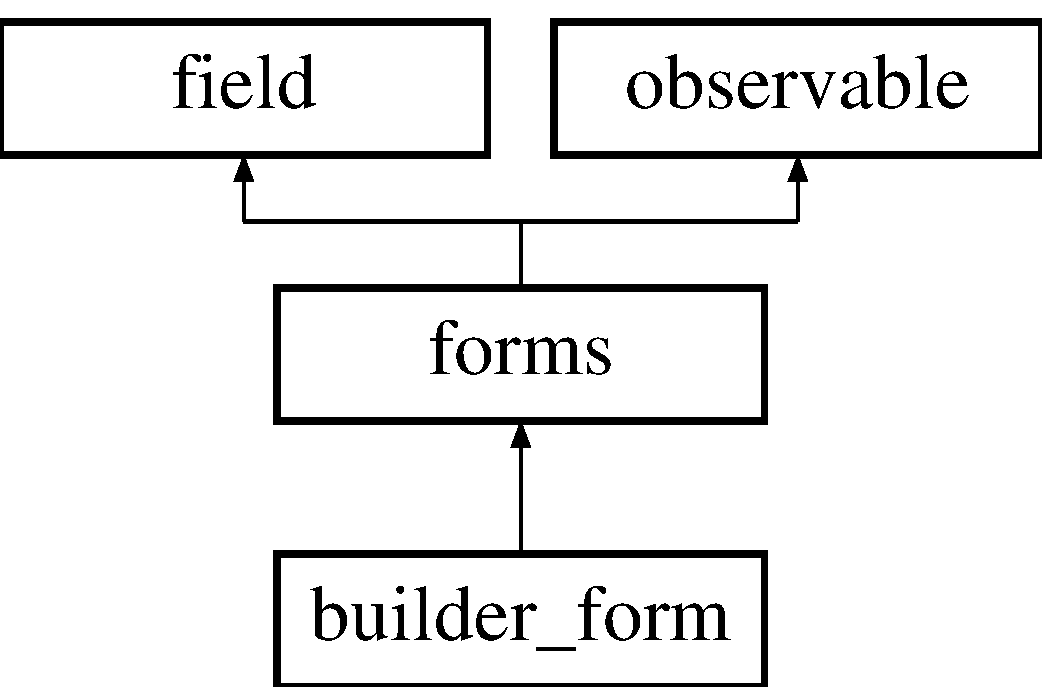
\includegraphics[height=3.000000cm]{classbuilder__form}
\end{center}
\end{figure}
\subsubsection*{Public Member Functions}
\begin{DoxyCompactItemize}
\item 
\hypertarget{classbuilder__form_a3ffef39ae7e16de827d3a1467b8085a2}{\hyperlink{classbuilder__form_a3ffef39ae7e16de827d3a1467b8085a2}{builder\-\_\-form} ()}\label{classbuilder__form_a3ffef39ae7e16de827d3a1467b8085a2}

\begin{DoxyCompactList}\small\item\em Constructor for the builder form. \end{DoxyCompactList}\item 
\hyperlink{classbuilder__form_a6408926fe73438032738d8a0095acf8d}{make\-\_\-field} ()
\begin{DoxyCompactList}\small\item\em Creates a field from this form to be added to the form we're building. \end{DoxyCompactList}\item 
\hyperlink{classbuilder__form_a250c986a9670cfe69371d854209991ba}{form} (\$errors)
\begin{DoxyCompactList}\small\item\em Returns the H\-T\-M\-L for this \hyperlink{classbuilder__form}{builder\-\_\-form}. \end{DoxyCompactList}\end{DoxyCompactItemize}
\subsubsection*{Additional Inherited Members}


\subsubsection{Detailed Description}
This file defines the builder forms, which builds other forms. 

This form build up a form by creating fields. 

\subsubsection{Member Function Documentation}
\hypertarget{classbuilder__form_a250c986a9670cfe69371d854209991ba}{\index{builder\-\_\-form@{builder\-\_\-form}!form@{form}}
\index{form@{form}!builder_form@{builder\-\_\-form}}
\paragraph[{form}]{\setlength{\rightskip}{0pt plus 5cm}builder\-\_\-form\-::form (
\begin{DoxyParamCaption}
\item[{}]{\$errors}
\end{DoxyParamCaption}
)}}\label{classbuilder__form_a250c986a9670cfe69371d854209991ba}


Returns the H\-T\-M\-L for this \hyperlink{classbuilder__form}{builder\-\_\-form}. 

\begin{DoxySeeAlso}{See Also}
\hyperlink{classforms_aca4fdeecf56bc5796f628a477f9ce629}{forms\-::form()} 
\end{DoxySeeAlso}


Implements \hyperlink{interfacefield_a1b51c4b8b01f77a26eda359e1fc0fb4c}{field}.

\hypertarget{classbuilder__form_a6408926fe73438032738d8a0095acf8d}{\index{builder\-\_\-form@{builder\-\_\-form}!make\-\_\-field@{make\-\_\-field}}
\index{make\-\_\-field@{make\-\_\-field}!builder_form@{builder\-\_\-form}}
\paragraph[{make\-\_\-field}]{\setlength{\rightskip}{0pt plus 5cm}builder\-\_\-form\-::make\-\_\-field (
\begin{DoxyParamCaption}
{}
\end{DoxyParamCaption}
)}}\label{classbuilder__form_a6408926fe73438032738d8a0095acf8d}


Creates a field from this form to be added to the form we're building. 

\begin{DoxyPrecond}{Precondition}
we have valid inputs, as checked with \hyperlink{classforms_a2494aca1309491b0ba423e233f4210b3}{sanitize()} and \hyperlink{classforms_a80d7d5c6d738b6f42cfbb258b3c3a3d1}{validate()} 
\end{DoxyPrecond}
\begin{DoxyReturn}{Returns}
an input object with the user set parameters. 
\end{DoxyReturn}


The documentation for this class was generated from the following file\-:\begin{DoxyCompactItemize}
\item 
builder\-\_\-form.\-inc.\-php\end{DoxyCompactItemize}

\hypertarget{classcolor__input}{\subsection{color\-\_\-input Class Reference}
\label{classcolor__input}\index{color\-\_\-input@{color\-\_\-input}}
}


This convience class creates a color input with validation and sanitization.  


Inheritance diagram for color\-\_\-input\-:\begin{figure}[H]
\begin{center}
\leavevmode
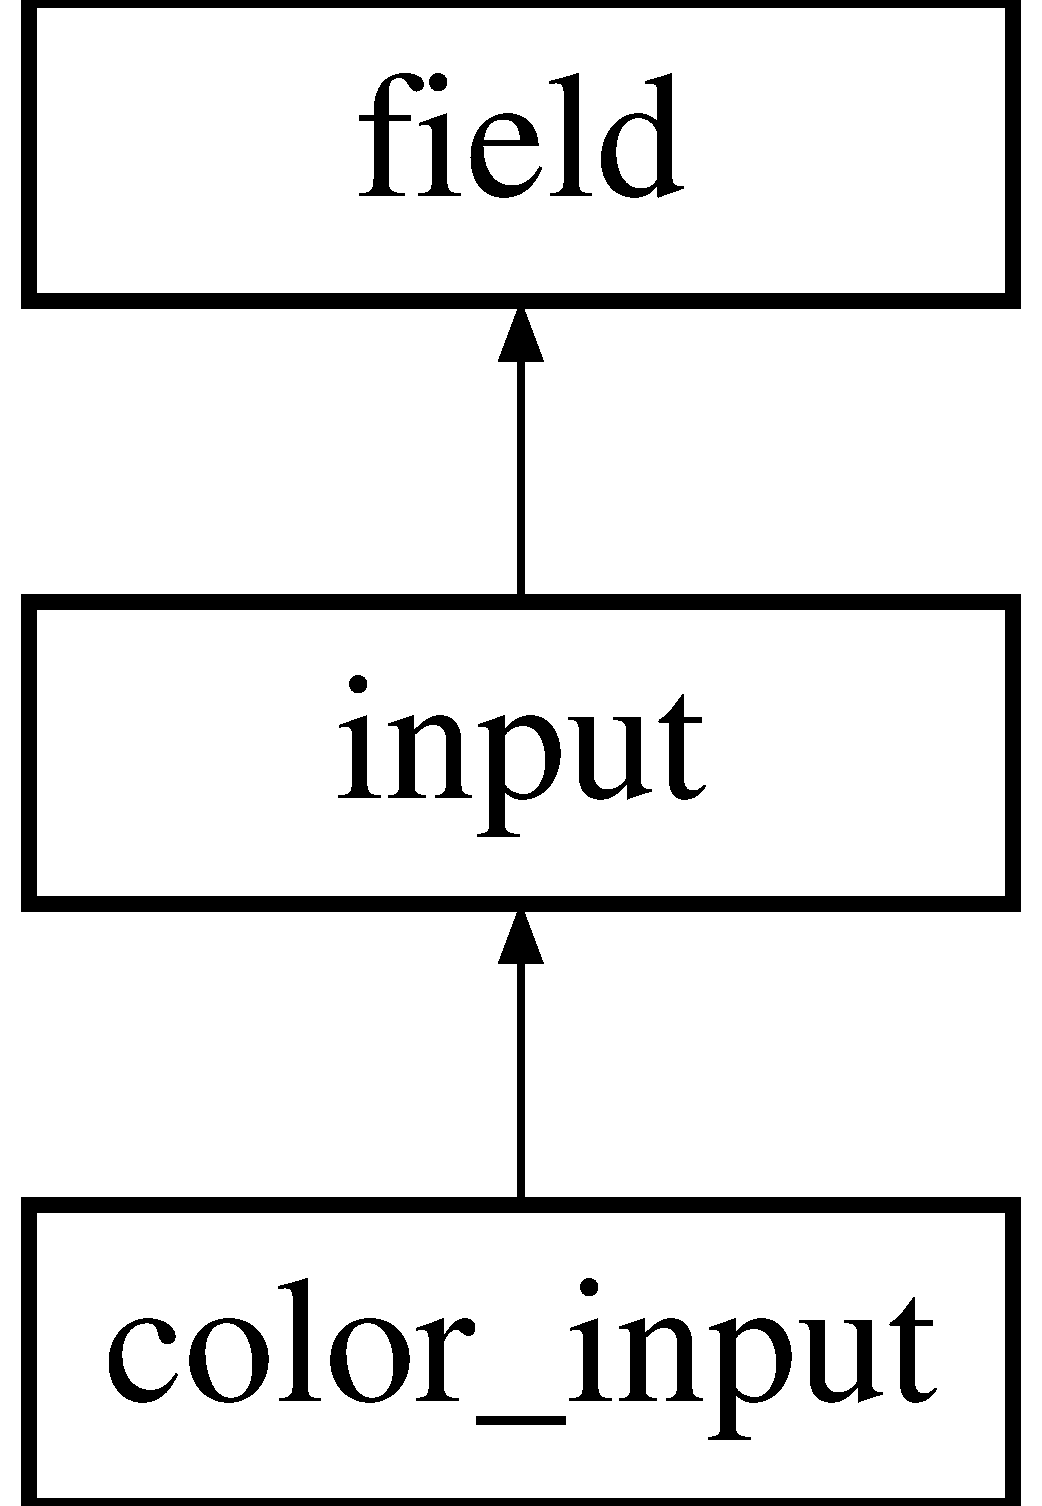
\includegraphics[height=3.000000cm]{classcolor__input}
\end{center}
\end{figure}
\subsubsection*{Public Member Functions}
\begin{DoxyCompactItemize}
\item 
\hypertarget{classcolor__input_ae7453daef5e053547d9ddb3c55ad4e1d}{{\bfseries \-\_\-\-\_\-construct} (\$label\-\_\-text, \$name, \$value, \$required=false, \$sanity\-\_\-func=null, \$valid\-\_\-func=null)}\label{classcolor__input_ae7453daef5e053547d9ddb3c55ad4e1d}

\end{DoxyCompactItemize}
\subsubsection*{Additional Inherited Members}


\subsubsection{Detailed Description}
This convience class creates a color input with validation and sanitization. 

The documentation for this class was generated from the following file\-:\begin{DoxyCompactItemize}
\item 
\hyperlink{extended__inputs_8inc_8php}{extended\-\_\-inputs.\-inc.\-php}\end{DoxyCompactItemize}

\hypertarget{interfacecrud}{\subsection{crud Interface Reference}
\label{interfacecrud}\index{crud@{crud}}
}


Describes an object that knows how to Create, Read, Update and Delete iteself.  


Inheritance diagram for crud\-:\begin{figure}[H]
\begin{center}
\leavevmode
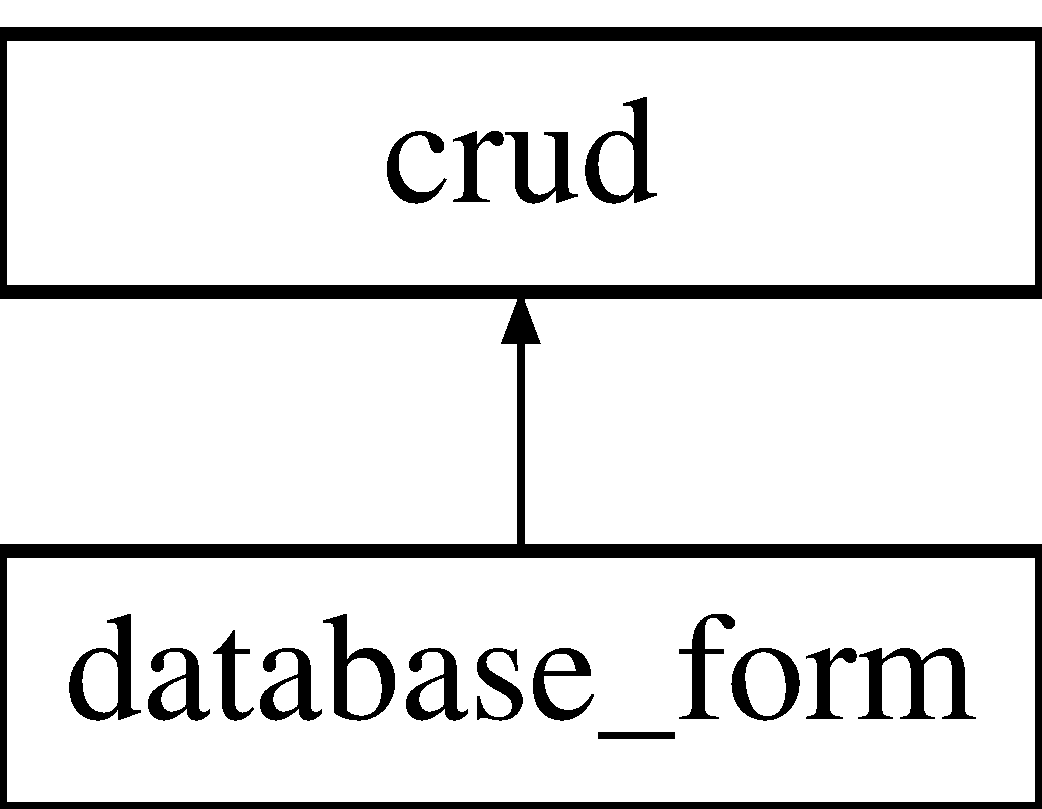
\includegraphics[height=2.000000cm]{interfacecrud}
\end{center}
\end{figure}
\subsubsection*{Public Member Functions}
\begin{DoxyCompactItemize}
\item 
\hyperlink{interfacecrud_aef5aaa8df2d390d2a96118dd3411fd1d}{create} ()
\begin{DoxyCompactList}\small\item\em Create \$this object in database or file. \end{DoxyCompactList}\item 
\hyperlink{interfacecrud_a9cbe80658a42208cee8825ad2a0db457}{read} ()
\begin{DoxyCompactList}\small\item\em Read the object from database into \$this object. \end{DoxyCompactList}\item 
\hyperlink{interfacecrud_a7e58697e70dc818f35ea1f548641a30d}{update} ()
\begin{DoxyCompactList}\small\item\em Update the record for \$this object. \end{DoxyCompactList}\item 
\hyperlink{interfacecrud_a1e74e05aa1d6785caadb51164df38f3b}{delete} ()
\begin{DoxyCompactList}\small\item\em Delete the record for \$this object. \end{DoxyCompactList}\end{DoxyCompactItemize}


\subsubsection{Detailed Description}
Describes an object that knows how to Create, Read, Update and Delete iteself. 

\subsubsection{Member Function Documentation}
\hypertarget{interfacecrud_aef5aaa8df2d390d2a96118dd3411fd1d}{\index{crud@{crud}!create@{create}}
\index{create@{create}!crud@{crud}}
\paragraph[{create}]{\setlength{\rightskip}{0pt plus 5cm}crud\-::create (
\begin{DoxyParamCaption}
{}
\end{DoxyParamCaption}
)}}\label{interfacecrud_aef5aaa8df2d390d2a96118dd3411fd1d}


Create \$this object in database or file. 

\begin{DoxyPostcond}{Postcondition}
\$this object is created in the storage medium. 
\end{DoxyPostcond}


Implemented in \hyperlink{classdatabase__form_a2f217d182a55038d501b66f2a2d51abc}{database\-\_\-form}.

\hypertarget{interfacecrud_a1e74e05aa1d6785caadb51164df38f3b}{\index{crud@{crud}!delete@{delete}}
\index{delete@{delete}!crud@{crud}}
\paragraph[{delete}]{\setlength{\rightskip}{0pt plus 5cm}crud\-::delete (
\begin{DoxyParamCaption}
{}
\end{DoxyParamCaption}
)}}\label{interfacecrud_a1e74e05aa1d6785caadb51164df38f3b}


Delete the record for \$this object. 

\begin{DoxyPostcond}{Postcondition}
The record for \$this object will be removed from the storage medium. 
\end{DoxyPostcond}


Implemented in \hyperlink{classdatabase__form_ac65c871bc6d3a45319bbb3f20901cc56}{database\-\_\-form}.

\hypertarget{interfacecrud_a9cbe80658a42208cee8825ad2a0db457}{\index{crud@{crud}!read@{read}}
\index{read@{read}!crud@{crud}}
\paragraph[{read}]{\setlength{\rightskip}{0pt plus 5cm}crud\-::read (
\begin{DoxyParamCaption}
{}
\end{DoxyParamCaption}
)}}\label{interfacecrud_a9cbe80658a42208cee8825ad2a0db457}


Read the object from database into \$this object. 

\begin{DoxyPostcond}{Postcondition}
If successful \$this object will have the data that was in the storage medium. 
\end{DoxyPostcond}


Implemented in \hyperlink{classdatabase__form_aff5e2b2b523b84443a34bc37472d5c8a}{database\-\_\-form}.

\hypertarget{interfacecrud_a7e58697e70dc818f35ea1f548641a30d}{\index{crud@{crud}!update@{update}}
\index{update@{update}!crud@{crud}}
\paragraph[{update}]{\setlength{\rightskip}{0pt plus 5cm}crud\-::update (
\begin{DoxyParamCaption}
{}
\end{DoxyParamCaption}
)}}\label{interfacecrud_a7e58697e70dc818f35ea1f548641a30d}


Update the record for \$this object. 

\begin{DoxyPostcond}{Postcondition}
The record for \$this object in the storage medium will be changed to match \$this object's current state. 
\end{DoxyPostcond}


Implemented in \hyperlink{classdatabase__form_a9c66a1a5dbd77ce0d110dd1672f74743}{database\-\_\-form}.



The documentation for this interface was generated from the following file\-:\begin{DoxyCompactItemize}
\item 
\hyperlink{crud_8inc_8php}{crud.\-inc.\-php}\end{DoxyCompactItemize}

\hypertarget{classdatabase__form}{\subsection{database\-\_\-form Class Reference}
\label{classdatabase__form}\index{database\-\_\-form@{database\-\_\-form}}
}


This class allows the both the structure and the data for this form to be written out to a database.  


Inheritance diagram for database\-\_\-form\-:\begin{figure}[H]
\begin{center}
\leavevmode
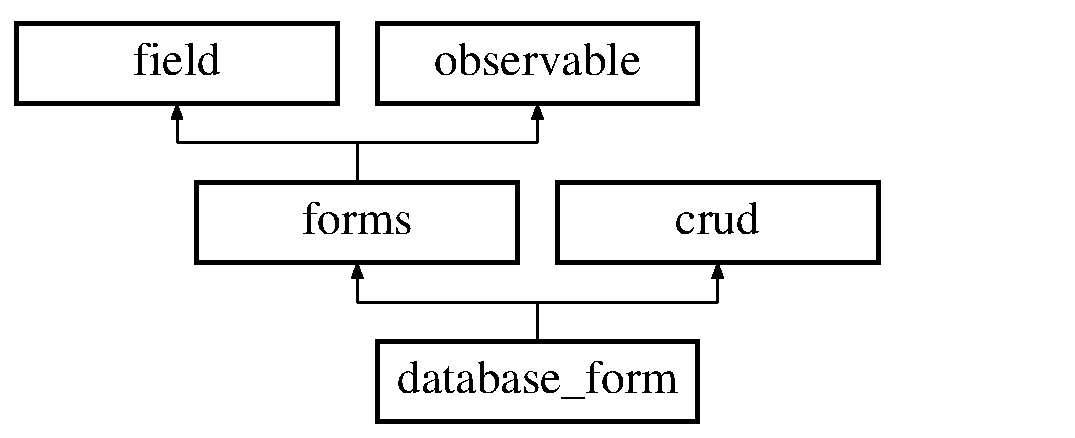
\includegraphics[height=3.000000cm]{classdatabase__form}
\end{center}
\end{figure}
\subsubsection*{Public Member Functions}
\begin{DoxyCompactItemize}
\item 
\hyperlink{classdatabase__form_a1d3ac5bd74951304e9be88700ac0dcda}{create\-\_\-form} ()
\begin{DoxyCompactList}\small\item\em Writes form structure into database \$db to table forms. \end{DoxyCompactList}\item 
\hyperlink{classdatabase__form_adb7962f1e12276e5d5d35d9bb43db0d6}{read\-\_\-form} ()
\begin{DoxyCompactList}\small\item\em Reads form structure out of database \$db table forms. \end{DoxyCompactList}\item 
\hyperlink{classdatabase__form_aae32575f2c15be7e82d574b01488292f}{update\-\_\-form} ()
\begin{DoxyCompactList}\small\item\em Writes form structure into database \$db to table forms. \end{DoxyCompactList}\item 
\hyperlink{classdatabase__form_a34c12094e361bdb922a5131a55826d28}{delete\-\_\-form} ()
\begin{DoxyCompactList}\small\item\em Delete this form from the database \$db table forms. \end{DoxyCompactList}\item 
\hyperlink{classdatabase__form_a2f217d182a55038d501b66f2a2d51abc}{create} ()
\begin{DoxyCompactList}\small\item\em Write the values of this form out to database \$db table forms\-\_\-data. \end{DoxyCompactList}\item 
\hyperlink{classdatabase__form_aff5e2b2b523b84443a34bc37472d5c8a}{read} ()
\begin{DoxyCompactList}\small\item\em Read the data into this form from database \$db table forms\-\_\-data. \end{DoxyCompactList}\item 
\hyperlink{classdatabase__form_a9c66a1a5dbd77ce0d110dd1672f74743}{update} ()
\begin{DoxyCompactList}\small\item\em Update the data in the database to match the values of this form. \end{DoxyCompactList}\item 
\hyperlink{classdatabase__form_ac65c871bc6d3a45319bbb3f20901cc56}{delete} ()
\begin{DoxyCompactList}\small\item\em Deletes the data record for this form. \end{DoxyCompactList}\item 
\hypertarget{classdatabase__form_ab973b6f65ef80102d3f49d589469de3c}{{\bfseries display\-\_\-structure} ()}\label{classdatabase__form_ab973b6f65ef80102d3f49d589469de3c}

\item 
\hyperlink{classdatabase__form_a73106bec9001ca0fe255e74a37982072}{display\-\_\-table} ()
\begin{DoxyCompactList}\small\item\em Returns H\-T\-M\-L for all form data for this specific form. \end{DoxyCompactList}\end{DoxyCompactItemize}
\subsubsection*{Additional Inherited Members}


\subsubsection{Detailed Description}
This class allows the both the structure and the data for this form to be written out to a database. 

\subsubsection{Member Function Documentation}
\hypertarget{classdatabase__form_a2f217d182a55038d501b66f2a2d51abc}{\index{database\-\_\-form@{database\-\_\-form}!create@{create}}
\index{create@{create}!database_form@{database\-\_\-form}}
\paragraph[{create}]{\setlength{\rightskip}{0pt plus 5cm}database\-\_\-form\-::create (
\begin{DoxyParamCaption}
{}
\end{DoxyParamCaption}
)}}\label{classdatabase__form_a2f217d182a55038d501b66f2a2d51abc}


Write the values of this form out to database \$db table forms\-\_\-data. 

\begin{DoxyPrecond}{Precondition}
Must have mysqli database connection object in scope named '\$db'. 
\end{DoxyPrecond}
\begin{DoxyPostcond}{Postcondition}
This forms data will be written out to the database. 
\end{DoxyPostcond}


Implements \hyperlink{interfacecrud_aef5aaa8df2d390d2a96118dd3411fd1d}{crud}.

\hypertarget{classdatabase__form_a1d3ac5bd74951304e9be88700ac0dcda}{\index{database\-\_\-form@{database\-\_\-form}!create\-\_\-form@{create\-\_\-form}}
\index{create\-\_\-form@{create\-\_\-form}!database_form@{database\-\_\-form}}
\paragraph[{create\-\_\-form}]{\setlength{\rightskip}{0pt plus 5cm}database\-\_\-form\-::create\-\_\-form (
\begin{DoxyParamCaption}
{}
\end{DoxyParamCaption}
)}}\label{classdatabase__form_a1d3ac5bd74951304e9be88700ac0dcda}


Writes form structure into database \$db to table forms. 

\begin{DoxyPrecond}{Precondition}
Must have mysqli database connection object in scope named '\$db'. 
\end{DoxyPrecond}
\begin{DoxyPostcond}{Postcondition}
The form in serialized form will be written to the database. 
\end{DoxyPostcond}
\hypertarget{classdatabase__form_ac65c871bc6d3a45319bbb3f20901cc56}{\index{database\-\_\-form@{database\-\_\-form}!delete@{delete}}
\index{delete@{delete}!database_form@{database\-\_\-form}}
\paragraph[{delete}]{\setlength{\rightskip}{0pt plus 5cm}database\-\_\-form\-::delete (
\begin{DoxyParamCaption}
{}
\end{DoxyParamCaption}
)}}\label{classdatabase__form_ac65c871bc6d3a45319bbb3f20901cc56}


Deletes the data record for this form. 

\begin{DoxyPrecond}{Precondition}
Must have mysqli database connection object in scope named '\$db'. 
\end{DoxyPrecond}
\begin{DoxyPostcond}{Postcondition}
The data for for this form will be deleted. 
\end{DoxyPostcond}


Implements \hyperlink{interfacecrud_a1e74e05aa1d6785caadb51164df38f3b}{crud}.

\hypertarget{classdatabase__form_a34c12094e361bdb922a5131a55826d28}{\index{database\-\_\-form@{database\-\_\-form}!delete\-\_\-form@{delete\-\_\-form}}
\index{delete\-\_\-form@{delete\-\_\-form}!database_form@{database\-\_\-form}}
\paragraph[{delete\-\_\-form}]{\setlength{\rightskip}{0pt plus 5cm}database\-\_\-form\-::delete\-\_\-form (
\begin{DoxyParamCaption}
{}
\end{DoxyParamCaption}
)}}\label{classdatabase__form_a34c12094e361bdb922a5131a55826d28}


Delete this form from the database \$db table forms. 

\begin{DoxyPrecond}{Precondition}
Must have mysqli database connection object in scope named '\$db'. 
\end{DoxyPrecond}
\begin{DoxyPostcond}{Postcondition}
this form will no loger be in the database. 
\end{DoxyPostcond}
\hypertarget{classdatabase__form_a73106bec9001ca0fe255e74a37982072}{\index{database\-\_\-form@{database\-\_\-form}!display\-\_\-table@{display\-\_\-table}}
\index{display\-\_\-table@{display\-\_\-table}!database_form@{database\-\_\-form}}
\paragraph[{display\-\_\-table}]{\setlength{\rightskip}{0pt plus 5cm}database\-\_\-form\-::display\-\_\-table (
\begin{DoxyParamCaption}
{}
\end{DoxyParamCaption}
)}}\label{classdatabase__form_a73106bec9001ca0fe255e74a37982072}


Returns H\-T\-M\-L for all form data for this specific form. 

\begin{DoxyPrecond}{Precondition}
Must have mysqli database connection object in scope named '\$db'. 
\end{DoxyPrecond}
\begin{DoxyReturn}{Returns}
array containting 'html' =$>$ The html table for all forms of this type filled out and 'js' =$>$ Any Java\-Script to make the table more functional. 
\end{DoxyReturn}
\hypertarget{classdatabase__form_aff5e2b2b523b84443a34bc37472d5c8a}{\index{database\-\_\-form@{database\-\_\-form}!read@{read}}
\index{read@{read}!database_form@{database\-\_\-form}}
\paragraph[{read}]{\setlength{\rightskip}{0pt plus 5cm}database\-\_\-form\-::read (
\begin{DoxyParamCaption}
{}
\end{DoxyParamCaption}
)}}\label{classdatabase__form_aff5e2b2b523b84443a34bc37472d5c8a}


Read the data into this form from database \$db table forms\-\_\-data. 

\begin{DoxyPrecond}{Precondition}
Must have mysqli database connection object in scope named '\$db'. 
\end{DoxyPrecond}
\begin{DoxyPostcond}{Postcondition}
This object will be populated with data from the database. 
\end{DoxyPostcond}


Implements \hyperlink{interfacecrud_a9cbe80658a42208cee8825ad2a0db457}{crud}.

\hypertarget{classdatabase__form_adb7962f1e12276e5d5d35d9bb43db0d6}{\index{database\-\_\-form@{database\-\_\-form}!read\-\_\-form@{read\-\_\-form}}
\index{read\-\_\-form@{read\-\_\-form}!database_form@{database\-\_\-form}}
\paragraph[{read\-\_\-form}]{\setlength{\rightskip}{0pt plus 5cm}database\-\_\-form\-::read\-\_\-form (
\begin{DoxyParamCaption}
{}
\end{DoxyParamCaption}
)}}\label{classdatabase__form_adb7962f1e12276e5d5d35d9bb43db0d6}


Reads form structure out of database \$db table forms. 

\begin{DoxyPrecond}{Precondition}
Must have mysqli database connection object in scope named '\$db'. 
\end{DoxyPrecond}
\begin{DoxyPostcond}{Postcondition}
This form will take on the structure that was saved to the database. 
\end{DoxyPostcond}
\hypertarget{classdatabase__form_a9c66a1a5dbd77ce0d110dd1672f74743}{\index{database\-\_\-form@{database\-\_\-form}!update@{update}}
\index{update@{update}!database_form@{database\-\_\-form}}
\paragraph[{update}]{\setlength{\rightskip}{0pt plus 5cm}database\-\_\-form\-::update (
\begin{DoxyParamCaption}
{}
\end{DoxyParamCaption}
)}}\label{classdatabase__form_a9c66a1a5dbd77ce0d110dd1672f74743}


Update the data in the database to match the values of this form. 

\begin{DoxyPrecond}{Precondition}
Must have mysqli database connection object in scope named '\$db'. 
\end{DoxyPrecond}
\begin{DoxyPostcond}{Postcondition}
the database records for the values of this form will be updated to match the values in this form. 
\end{DoxyPostcond}


Implements \hyperlink{interfacecrud_a7e58697e70dc818f35ea1f548641a30d}{crud}.

\hypertarget{classdatabase__form_aae32575f2c15be7e82d574b01488292f}{\index{database\-\_\-form@{database\-\_\-form}!update\-\_\-form@{update\-\_\-form}}
\index{update\-\_\-form@{update\-\_\-form}!database_form@{database\-\_\-form}}
\paragraph[{update\-\_\-form}]{\setlength{\rightskip}{0pt plus 5cm}database\-\_\-form\-::update\-\_\-form (
\begin{DoxyParamCaption}
{}
\end{DoxyParamCaption}
)}}\label{classdatabase__form_aae32575f2c15be7e82d574b01488292f}


Writes form structure into database \$db to table forms. 

\begin{DoxyPrecond}{Precondition}
Must have mysqli database connection object in scope named '\$db'. 
\end{DoxyPrecond}
\begin{DoxyPostcond}{Postcondition}
The form in serialized form will be written to the database. 
\end{DoxyPostcond}


The documentation for this class was generated from the following file\-:\begin{DoxyCompactItemize}
\item 
\hyperlink{database__form_8inc_8php}{database\-\_\-form.\-inc.\-php}\end{DoxyCompactItemize}

\hypertarget{classdatalist__input}{\subsection{datalist\-\_\-input Class Reference}
\label{classdatalist__input}\index{datalist\-\_\-input@{datalist\-\_\-input}}
}


Adaptor to input class, adds a datalist.  


Inheritance diagram for datalist\-\_\-input\-:\begin{figure}[H]
\begin{center}
\leavevmode
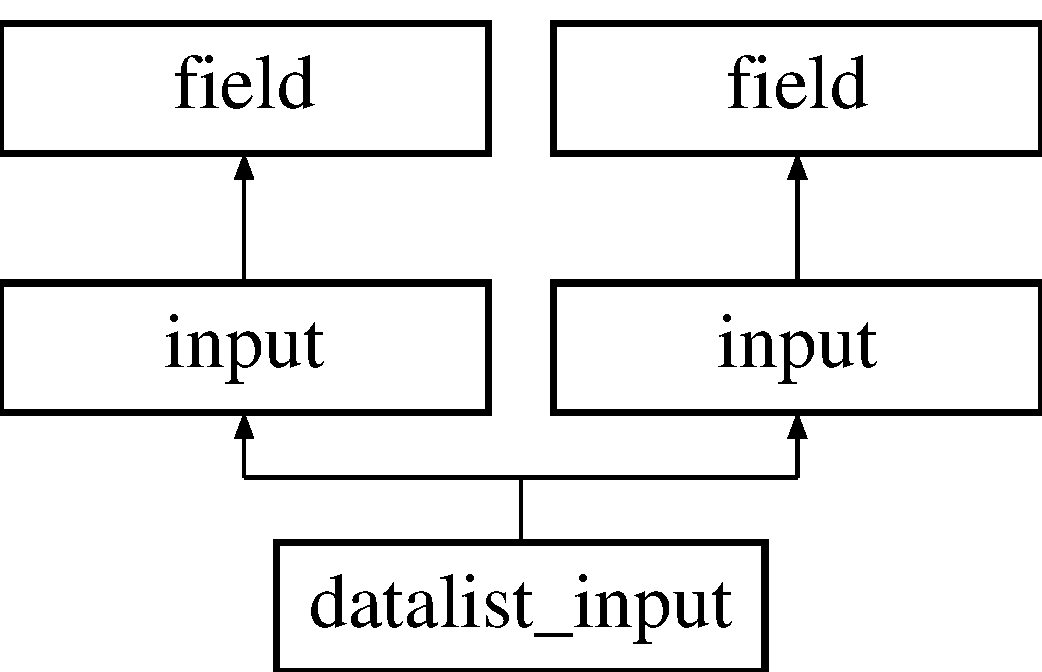
\includegraphics[height=3.000000cm]{classdatalist__input}
\end{center}
\end{figure}
\subsubsection*{Public Member Functions}
\begin{DoxyCompactItemize}
\item 
\hyperlink{classdatalist__input_aba53bff8ed66c85b97ce1ff23bfc15ec}{form} (\$errors=array())
\begin{DoxyCompactList}\small\item\em Generates the html for the input for inclusion in a form. \end{DoxyCompactList}\item 
\hyperlink{classdatalist__input_a5d082a8f7ebee9b5835490d75128c7e1}{datalist\-\_\-input} (\$\hyperlink{classinput}{input}, \$datalist)
\begin{DoxyCompactList}\small\item\em Constructor. \end{DoxyCompactList}\item 
\hyperlink{classdatalist__input_a6f94bf1247bd5da6f79c864b18073ed5}{display} ()
\begin{DoxyCompactList}\small\item\em Display function wraps \hyperlink{classinput_a993053ef011cade1db0ceaccb1f4da53}{input\-::display()} \end{DoxyCompactList}\item 
\hyperlink{classdatalist__input_a52e50cc544ff141a03c2fc65bfdaf9ea}{sanitize} ()
\begin{DoxyCompactList}\small\item\em Sanitization function wraps \hyperlink{classinput_ab8456d2b5a929801af6fe0b36afd458c}{input\-::sanitize()} \end{DoxyCompactList}\item 
\hyperlink{classdatalist__input_ab2827973f443100315d378d4a97b9516}{validate} (\$errors=array())
\begin{DoxyCompactList}\small\item\em Validation function wraps input\-::valudate() \end{DoxyCompactList}\item 
\hyperlink{classdatalist__input_afeb3a182794c4fb9c235c888b2029430}{get\-\_\-value} ()
\begin{DoxyCompactList}\small\item\em Inspector for value of input, wraps \hyperlink{classinput_a1b3bcdbb596a1154a944a169ac67f547}{input\-::get\-\_\-value()} \end{DoxyCompactList}\item 
\hyperlink{classdatalist__input_a73b5d2cfe2f300a62a39f5dfd5a18e70}{set\-\_\-value} (\$v)
\begin{DoxyCompactList}\small\item\em Mutator function wraps \hyperlink{classinput_a2383e00d55bf3dbcc7071b2fe1336aec}{input\-::set\-\_\-value()} \end{DoxyCompactList}\end{DoxyCompactItemize}
\subsubsection*{Additional Inherited Members}


\subsubsection{Detailed Description}
Adaptor to input class, adds a datalist. 

\subsubsection{Member Function Documentation}
\hypertarget{classdatalist__input_a5d082a8f7ebee9b5835490d75128c7e1}{\index{datalist\-\_\-input@{datalist\-\_\-input}!datalist\-\_\-input@{datalist\-\_\-input}}
\index{datalist\-\_\-input@{datalist\-\_\-input}!datalist_input@{datalist\-\_\-input}}
\paragraph[{datalist\-\_\-input}]{\setlength{\rightskip}{0pt plus 5cm}datalist\-\_\-input\-::datalist\-\_\-input (
\begin{DoxyParamCaption}
\item[{}]{\$input, }
\item[{}]{\$datalist}
\end{DoxyParamCaption}
)}}\label{classdatalist__input_a5d082a8f7ebee9b5835490d75128c7e1}


Constructor. 


\begin{DoxyParams}[1]{Parameters}
input & {\em \$input} & The input we are wrapping \\
\hline
array & {\em \$datalist} & The list of values we want in the datalist \\
\hline
\end{DoxyParams}
\hypertarget{classdatalist__input_a6f94bf1247bd5da6f79c864b18073ed5}{\index{datalist\-\_\-input@{datalist\-\_\-input}!display@{display}}
\index{display@{display}!datalist_input@{datalist\-\_\-input}}
\paragraph[{display}]{\setlength{\rightskip}{0pt plus 5cm}datalist\-\_\-input\-::display (
\begin{DoxyParamCaption}
{}
\end{DoxyParamCaption}
)}}\label{classdatalist__input_a6f94bf1247bd5da6f79c864b18073ed5}


Display function wraps \hyperlink{classinput_a993053ef011cade1db0ceaccb1f4da53}{input\-::display()} 

\begin{DoxyReturn}{Returns}
A string containing the formated name value pair for this input. 
\end{DoxyReturn}
\begin{DoxySeeAlso}{See Also}
\hyperlink{classinput_a993053ef011cade1db0ceaccb1f4da53}{input\-::display()} 
\end{DoxySeeAlso}


Implements \hyperlink{interfacefield_a6a8bbd656a0e7cab2604f6df859bb60a}{field}.

\hypertarget{classdatalist__input_aba53bff8ed66c85b97ce1ff23bfc15ec}{\index{datalist\-\_\-input@{datalist\-\_\-input}!form@{form}}
\index{form@{form}!datalist_input@{datalist\-\_\-input}}
\paragraph[{form}]{\setlength{\rightskip}{0pt plus 5cm}datalist\-\_\-input\-::form (
\begin{DoxyParamCaption}
\item[{}]{\$errors = {\ttfamily array()}}
\end{DoxyParamCaption}
)}}\label{classdatalist__input_aba53bff8ed66c85b97ce1ff23bfc15ec}


Generates the html for the input for inclusion in a form. 


\begin{DoxyParams}[1]{Parameters}
array & {\em \$errors} & an accoiated array errors. If the field name appears in errors, the field's label will be a class of error. \\
\hline
\end{DoxyParams}
\begin{DoxyReturn}{Returns}
array with two elements 'html' the H\-T\-M\-L of the input field and 'js' any Java\-Script that would assoicated with it (empty for basic input types at this time). 
\end{DoxyReturn}
\begin{DoxyRefDesc}{Todo}
\item[\hyperlink{todo__todo000006}{Todo}]fix so it doesn't require J\-S. \end{DoxyRefDesc}


Implements \hyperlink{interfacefield_a1b51c4b8b01f77a26eda359e1fc0fb4c}{field}.

\hypertarget{classdatalist__input_afeb3a182794c4fb9c235c888b2029430}{\index{datalist\-\_\-input@{datalist\-\_\-input}!get\-\_\-value@{get\-\_\-value}}
\index{get\-\_\-value@{get\-\_\-value}!datalist_input@{datalist\-\_\-input}}
\paragraph[{get\-\_\-value}]{\setlength{\rightskip}{0pt plus 5cm}datalist\-\_\-input\-::get\-\_\-value (
\begin{DoxyParamCaption}
{}
\end{DoxyParamCaption}
)}}\label{classdatalist__input_afeb3a182794c4fb9c235c888b2029430}


Inspector for value of input, wraps \hyperlink{classinput_a1b3bcdbb596a1154a944a169ac67f547}{input\-::get\-\_\-value()} 

\begin{DoxyReturn}{Returns}
the current value of \$this input 
\end{DoxyReturn}
\hypertarget{classdatalist__input_a52e50cc544ff141a03c2fc65bfdaf9ea}{\index{datalist\-\_\-input@{datalist\-\_\-input}!sanitize@{sanitize}}
\index{sanitize@{sanitize}!datalist_input@{datalist\-\_\-input}}
\paragraph[{sanitize}]{\setlength{\rightskip}{0pt plus 5cm}datalist\-\_\-input\-::sanitize (
\begin{DoxyParamCaption}
{}
\end{DoxyParamCaption}
)}}\label{classdatalist__input_a52e50cc544ff141a03c2fc65bfdaf9ea}


Sanitization function wraps \hyperlink{classinput_ab8456d2b5a929801af6fe0b36afd458c}{input\-::sanitize()} 

\begin{DoxySeeAlso}{See Also}
\hyperlink{classinput_ab8456d2b5a929801af6fe0b36afd458c}{input\-::sanitize} 
\end{DoxySeeAlso}


Implements \hyperlink{interfacefield_a3ed132df10731b5ebe33acc44ac03c85}{field}.

\hypertarget{classdatalist__input_a73b5d2cfe2f300a62a39f5dfd5a18e70}{\index{datalist\-\_\-input@{datalist\-\_\-input}!set\-\_\-value@{set\-\_\-value}}
\index{set\-\_\-value@{set\-\_\-value}!datalist_input@{datalist\-\_\-input}}
\paragraph[{set\-\_\-value}]{\setlength{\rightskip}{0pt plus 5cm}datalist\-\_\-input\-::set\-\_\-value (
\begin{DoxyParamCaption}
\item[{}]{\$v}
\end{DoxyParamCaption}
)}}\label{classdatalist__input_a73b5d2cfe2f300a62a39f5dfd5a18e70}


Mutator function wraps \hyperlink{classinput_a2383e00d55bf3dbcc7071b2fe1336aec}{input\-::set\-\_\-value()} 


\begin{DoxyParams}[1]{Parameters}
mixed & {\em \$v} & The new value of this input \\
\hline
\end{DoxyParams}
\hypertarget{classdatalist__input_ab2827973f443100315d378d4a97b9516}{\index{datalist\-\_\-input@{datalist\-\_\-input}!validate@{validate}}
\index{validate@{validate}!datalist_input@{datalist\-\_\-input}}
\paragraph[{validate}]{\setlength{\rightskip}{0pt plus 5cm}datalist\-\_\-input\-::validate (
\begin{DoxyParamCaption}
\item[{}]{\$errors = {\ttfamily array()}}
\end{DoxyParamCaption}
)}}\label{classdatalist__input_ab2827973f443100315d378d4a97b9516}


Validation function wraps input\-::valudate() 


\begin{DoxyParams}[1]{Parameters}
array & {\em \$errors} & an array of errors previously in the form, errors will be added to the array and the array returned. @ return array errors is returned, possibly with errors appended. \\
\hline
\end{DoxyParams}
\begin{DoxySeeAlso}{See Also}
\hyperlink{classinput_aaf4ed91e7abbc20e2396a4b07dbd031a}{input\-::validate()} 
\end{DoxySeeAlso}


Implements \hyperlink{interfacefield_a352b92f9e8dce69191bad79bdc5d972b}{field}.



The documentation for this class was generated from the following file\-:\begin{DoxyCompactItemize}
\item 
\hyperlink{extended__inputs_8inc_8php}{extended\-\_\-inputs.\-inc.\-php}\end{DoxyCompactItemize}

\hypertarget{classdate__input}{\subsection{date\-\_\-input Class Reference}
\label{classdate__input}\index{date\-\_\-input@{date\-\_\-input}}
}


This convience class creates a date input.  


Inheritance diagram for date\-\_\-input\-:\begin{figure}[H]
\begin{center}
\leavevmode
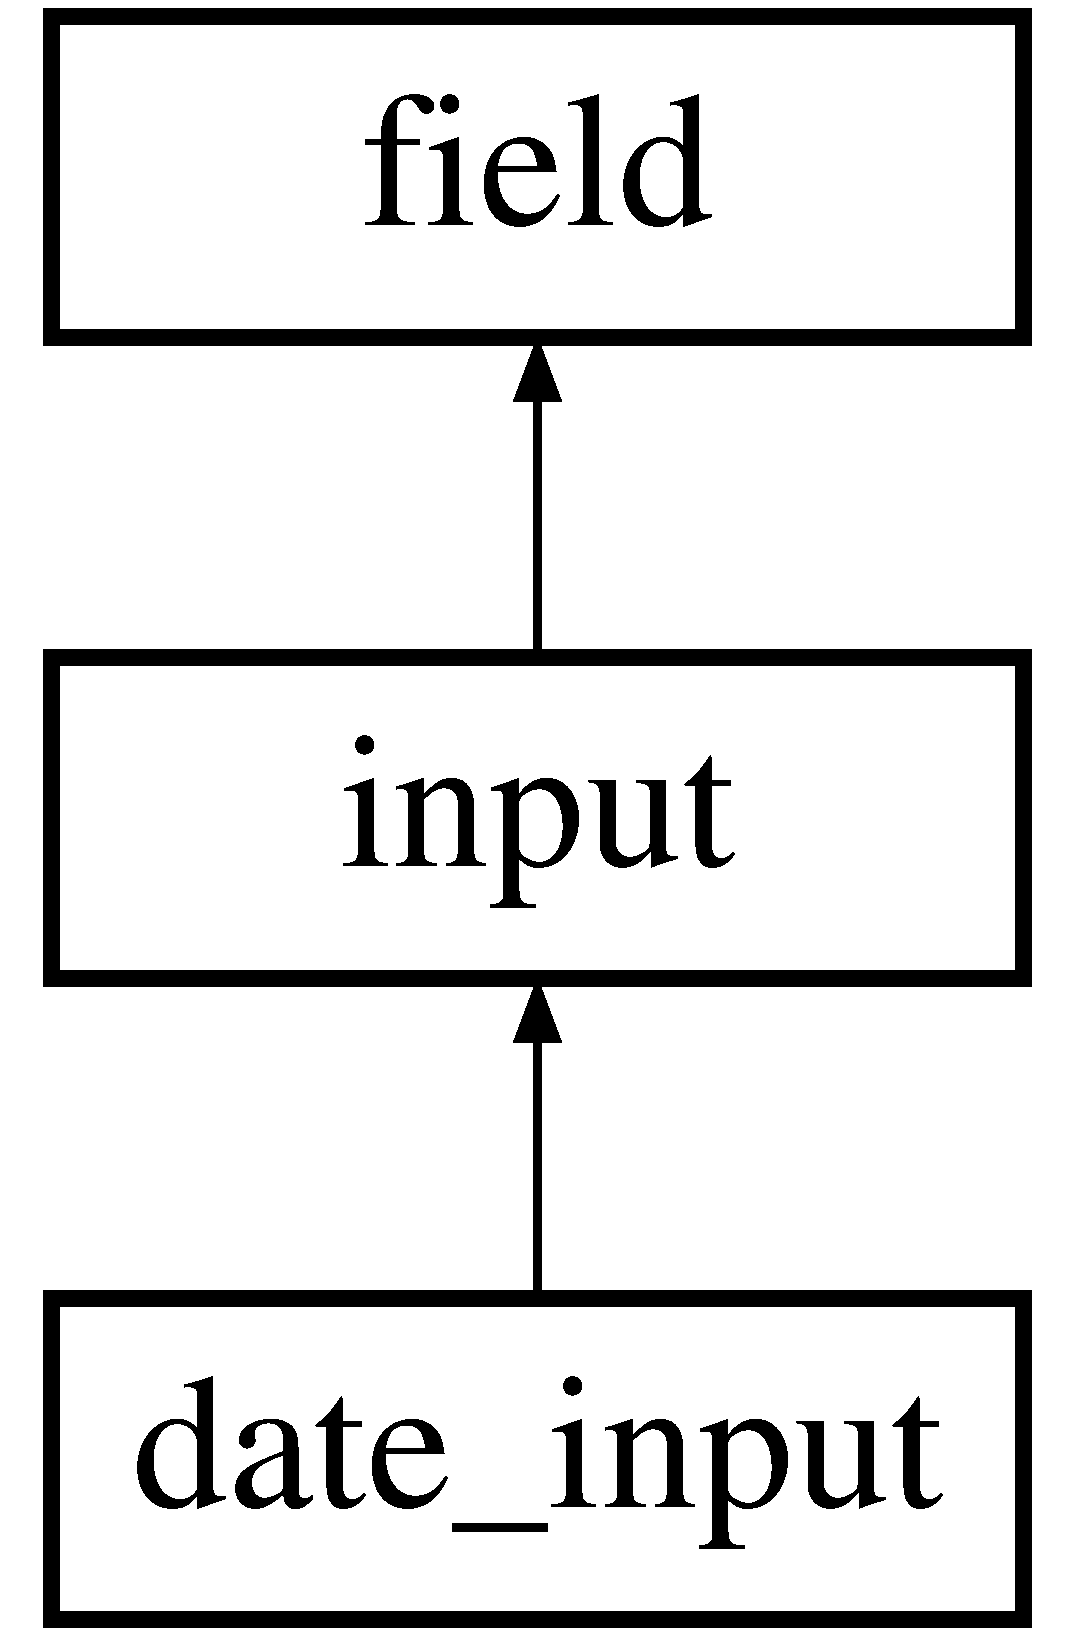
\includegraphics[height=3.000000cm]{classdate__input}
\end{center}
\end{figure}
\subsubsection*{Public Member Functions}
\begin{DoxyCompactItemize}
\item 
\hyperlink{classdate__input_a492b84dcbc8228427c6e5b0c415ad7ed}{date\-\_\-input} (\$label\-\_\-text, \$name, \$value, \$required=false, \$min= '', \$max= '', \$sanity\-\_\-func=null, \$valid\-\_\-func=null)
\begin{DoxyCompactList}\small\item\em constructor for \hyperlink{classdate__input}{date\-\_\-input} \end{DoxyCompactList}\end{DoxyCompactItemize}
\subsubsection*{Additional Inherited Members}


\subsubsection{Detailed Description}
This convience class creates a date input. 

\begin{DoxyRefDesc}{Todo}
\item[\hyperlink{todo__todo000005}{Todo}]Polyfill. \end{DoxyRefDesc}


\subsubsection{Member Function Documentation}
\hypertarget{classdate__input_a492b84dcbc8228427c6e5b0c415ad7ed}{\index{date\-\_\-input@{date\-\_\-input}!date\-\_\-input@{date\-\_\-input}}
\index{date\-\_\-input@{date\-\_\-input}!date_input@{date\-\_\-input}}
\paragraph[{date\-\_\-input}]{\setlength{\rightskip}{0pt plus 5cm}date\-\_\-input\-::date\-\_\-input (
\begin{DoxyParamCaption}
\item[{}]{\$label\-\_\-text, }
\item[{}]{\$name, }
\item[{}]{\$value, }
\item[{}]{\$required = {\ttfamily false}, }
\item[{}]{\$min = {\ttfamily ''}, }
\item[{}]{\$max = {\ttfamily ''}, }
\item[{}]{\$sanity\-\_\-func = {\ttfamily null}, }
\item[{}]{\$valid\-\_\-func = {\ttfamily null}}
\end{DoxyParamCaption}
)}}\label{classdate__input_a492b84dcbc8228427c6e5b0c415ad7ed}


constructor for \hyperlink{classdate__input}{date\-\_\-input} 


\begin{DoxyParams}[1]{Parameters}
string & {\em \$label\-\_\-text} & The text label for this \hyperlink{classzip__input}{zip\-\_\-input}. \\
\hline
string & {\em \$name} & The name of this field for internal use. (i.\-e. the name attribute in the render H\-T\-M\-L and/or used in form) \\
\hline
string & {\em \$value} & The current value of this input. Optional. Default is ''. \\
\hline
bool & {\em \$required} & Weather or not the user is required to enter this field. This effects both H\-T\-M\-L5 element and validation. Optional. Default is false. \\
\hline
string & {\em \$min} & a string representing the minimum date. Optional. \\
\hline
string & {\em \$max} & a string representing the maximum date. Optional. \\
\hline
 & {\em \$sanity\-\_\-func} & Optional function for sanitization. Defualt is null. \\
\hline
 & {\em \$valid\-\_\-func} & Optional function for validation. Default is null. \\
\hline
\end{DoxyParams}


The documentation for this class was generated from the following file\-:\begin{DoxyCompactItemize}
\item 
\hyperlink{extended__inputs_8inc_8php}{extended\-\_\-inputs.\-inc.\-php}\end{DoxyCompactItemize}

\hypertarget{classdb__form}{\subsection{db\-\_\-form Class Reference}
\label{classdb__form}\index{db\-\_\-form@{db\-\_\-form}}
}


Represents an H\-T\-M\-L form, and saves form data in \$db table named by the name attribue of this object.  


Inheritance diagram for db\-\_\-form\-:\begin{figure}[H]
\begin{center}
\leavevmode
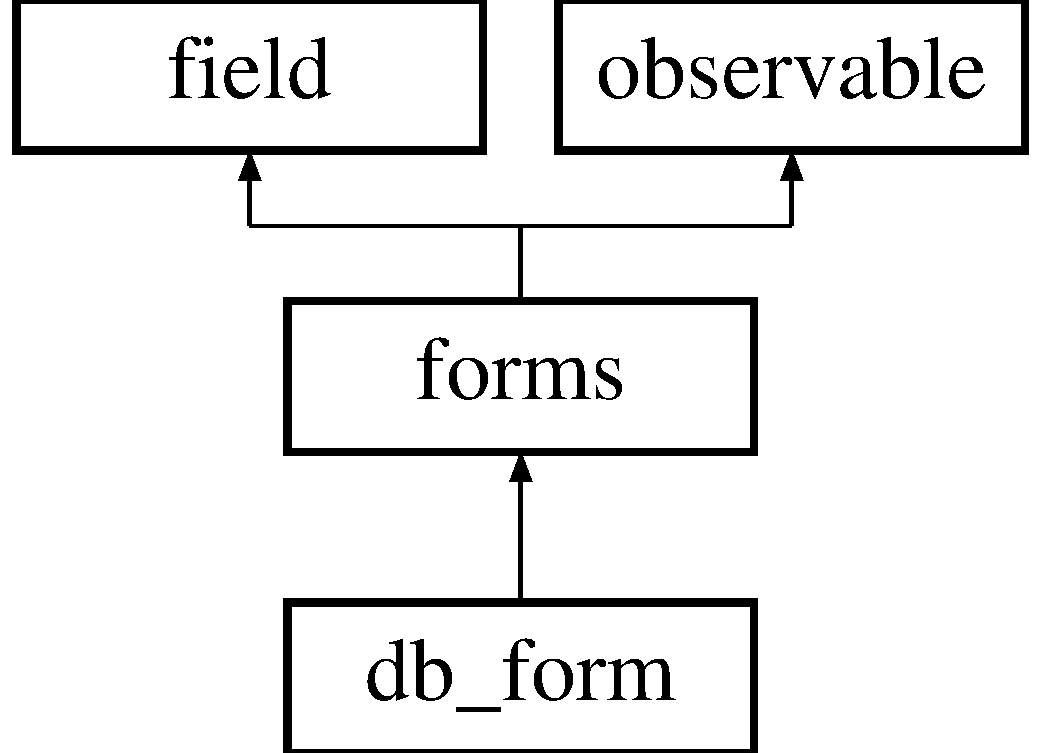
\includegraphics[height=3.000000cm]{classdb__form}
\end{center}
\end{figure}
\subsubsection*{Public Member Functions}
\begin{DoxyCompactItemize}
\item 
\hyperlink{classdb__form_af9e3c532c73b0c3bf82996e54f0390c7}{create} ()
\begin{DoxyCompactList}\small\item\em Inserts new record into database \$db table $<$name$>$. \end{DoxyCompactList}\item 
\hyperlink{classdb__form_aa77f60c8ca3cd52f28ea455eaa2f633d}{read} ()
\begin{DoxyCompactList}\small\item\em Reads an object back from database table $<$name$>$. \end{DoxyCompactList}\item 
\hyperlink{classdb__form_a132f6a150aad88391ce063711c08ace3}{update} ()
\begin{DoxyCompactList}\small\item\em Updates the base record for this form. \end{DoxyCompactList}\item 
\hyperlink{classdb__form_a09bce6f14faa4db14589a8627c782b4c}{delete} ()
\begin{DoxyCompactList}\small\item\em Deletes the record for this form. \end{DoxyCompactList}\item 
\hyperlink{classdb__form_a39893c90e5b3364fdae768079ff66520}{create\-\_\-sql} ()
\begin{DoxyCompactList}\small\item\em Generates and returns the S\-Q\-L to create the table for this form. \end{DoxyCompactList}\end{DoxyCompactItemize}
\subsubsection*{Additional Inherited Members}


\subsubsection{Detailed Description}
Represents an H\-T\-M\-L form, and saves form data in \$db table named by the name attribue of this object. 

\begin{DoxyRefDesc}{Todo}
\item[\hyperlink{todo__todo000001}{Todo}]\-: decide it this is the way to do this. perhaps write the alternative menthod. \end{DoxyRefDesc}


\subsubsection{Member Function Documentation}
\hypertarget{classdb__form_af9e3c532c73b0c3bf82996e54f0390c7}{\index{db\-\_\-form@{db\-\_\-form}!create@{create}}
\index{create@{create}!db_form@{db\-\_\-form}}
\paragraph[{create}]{\setlength{\rightskip}{0pt plus 5cm}db\-\_\-form\-::create (
\begin{DoxyParamCaption}
{}
\end{DoxyParamCaption}
)}}\label{classdb__form_af9e3c532c73b0c3bf82996e54f0390c7}


Inserts new record into database \$db table $<$name$>$. 

\begin{DoxyPrecond}{Precondition}
\$db must be a mysqli connection and $<$name$>$ must exist 
\end{DoxyPrecond}
\hypertarget{classdb__form_a39893c90e5b3364fdae768079ff66520}{\index{db\-\_\-form@{db\-\_\-form}!create\-\_\-sql@{create\-\_\-sql}}
\index{create\-\_\-sql@{create\-\_\-sql}!db_form@{db\-\_\-form}}
\paragraph[{create\-\_\-sql}]{\setlength{\rightskip}{0pt plus 5cm}db\-\_\-form\-::create\-\_\-sql (
\begin{DoxyParamCaption}
{}
\end{DoxyParamCaption}
)}}\label{classdb__form_a39893c90e5b3364fdae768079ff66520}


Generates and returns the S\-Q\-L to create the table for this form. 

\begin{DoxyRefDesc}{Todo}
\item[\hyperlink{todo__todo000004}{Todo}]\end{DoxyRefDesc}
\hypertarget{classdb__form_a09bce6f14faa4db14589a8627c782b4c}{\index{db\-\_\-form@{db\-\_\-form}!delete@{delete}}
\index{delete@{delete}!db_form@{db\-\_\-form}}
\paragraph[{delete}]{\setlength{\rightskip}{0pt plus 5cm}db\-\_\-form\-::delete (
\begin{DoxyParamCaption}
{}
\end{DoxyParamCaption}
)}}\label{classdb__form_a09bce6f14faa4db14589a8627c782b4c}


Deletes the record for this form. 

\begin{DoxyPrecond}{Precondition}
\$db must be a mysqli connection and $<$name$>$ must exist 
\end{DoxyPrecond}
\begin{DoxyRefDesc}{Todo}
\item[\hyperlink{todo__todo000003}{Todo}]\end{DoxyRefDesc}
\hypertarget{classdb__form_aa77f60c8ca3cd52f28ea455eaa2f633d}{\index{db\-\_\-form@{db\-\_\-form}!read@{read}}
\index{read@{read}!db_form@{db\-\_\-form}}
\paragraph[{read}]{\setlength{\rightskip}{0pt plus 5cm}db\-\_\-form\-::read (
\begin{DoxyParamCaption}
{}
\end{DoxyParamCaption}
)}}\label{classdb__form_aa77f60c8ca3cd52f28ea455eaa2f633d}


Reads an object back from database table $<$name$>$. 

\begin{DoxyPrecond}{Precondition}
\$db must be a mysqli connection and $<$name$>$ must exist 
\end{DoxyPrecond}
\hypertarget{classdb__form_a132f6a150aad88391ce063711c08ace3}{\index{db\-\_\-form@{db\-\_\-form}!update@{update}}
\index{update@{update}!db_form@{db\-\_\-form}}
\paragraph[{update}]{\setlength{\rightskip}{0pt plus 5cm}db\-\_\-form\-::update (
\begin{DoxyParamCaption}
{}
\end{DoxyParamCaption}
)}}\label{classdb__form_a132f6a150aad88391ce063711c08ace3}


Updates the base record for this form. 

\begin{DoxyPrecond}{Precondition}
\$db must be a mysqli connection and $<$name$>$ must exist 
\end{DoxyPrecond}
\begin{DoxyRefDesc}{Todo}
\item[\hyperlink{todo__todo000002}{Todo}]\end{DoxyRefDesc}


The documentation for this class was generated from the following file\-:\begin{DoxyCompactItemize}
\item 
\hyperlink{db__form_8inc_8php}{db\-\_\-form.\-inc.\-php}\end{DoxyCompactItemize}

\hypertarget{classemail__form__values}{\subsection{email\-\_\-form\-\_\-values Class Reference}
\label{classemail__form__values}\index{email\-\_\-form\-\_\-values@{email\-\_\-form\-\_\-values}}
}
Inheritance diagram for email\-\_\-form\-\_\-values\-:\begin{figure}[H]
\begin{center}
\leavevmode
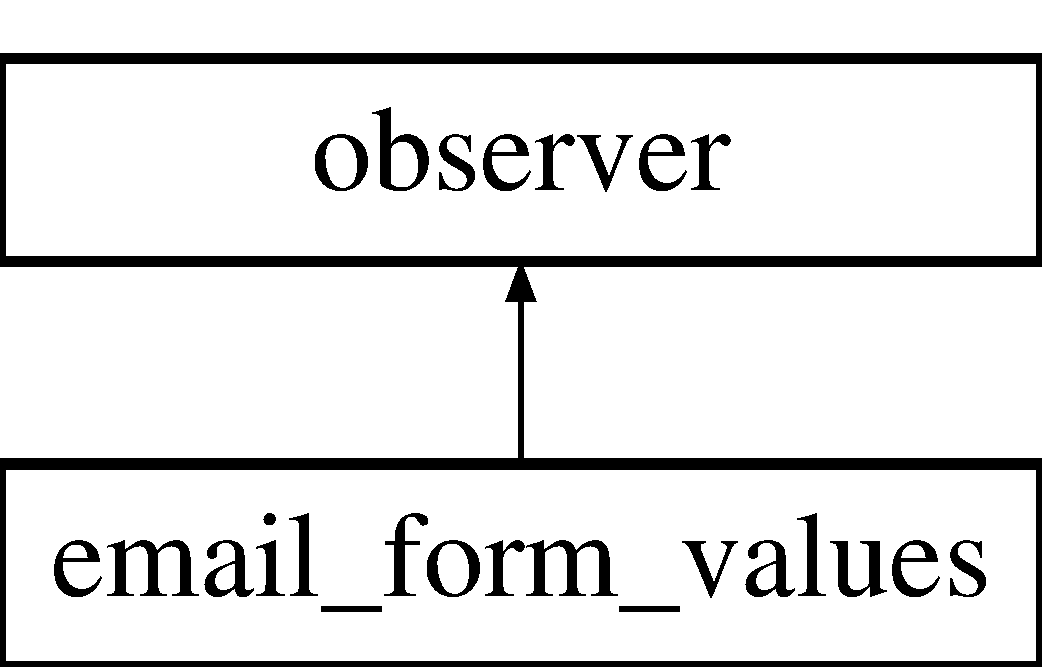
\includegraphics[height=2.000000cm]{classemail__form__values}
\end{center}
\end{figure}
\subsubsection*{Public Member Functions}
\begin{DoxyCompactItemize}
\item 
\hypertarget{classemail__form__values_a0f34f9d698413cced7d71f70e56bc2ae}{{\bfseries email\-\_\-form\-\_\-values} (\$email\-\_\-to= '', \$email\-\_\-from= '', \$email\-\_\-subject= '', \$condition=null)}\label{classemail__form__values_a0f34f9d698413cced7d71f70e56bc2ae}

\item 
\hypertarget{classemail__form__values_aa5aaf3b2f99af03834b3c12b04e3dd29}{{\bfseries notify} (\$\hyperlink{classevent}{event})}\label{classemail__form__values_aa5aaf3b2f99af03834b3c12b04e3dd29}

\item 
\hypertarget{classemail__form__values_ac366707f802e46865a9bf363c35f3841}{{\bfseries values} (\$v)}\label{classemail__form__values_ac366707f802e46865a9bf363c35f3841}

\item 
\hypertarget{classemail__form__values_a740b9cbf52273cdb99899964076aed64}{{\bfseries form} (\$the\-\_\-form)}\label{classemail__form__values_a740b9cbf52273cdb99899964076aed64}

\end{DoxyCompactItemize}
\subsubsection*{Public Attributes}
\begin{DoxyCompactItemize}
\item 
\hypertarget{classemail__form__values_a9dc3bcda67c6991a1921625bb98104b2}{{\bfseries \$email\-\_\-to}}\label{classemail__form__values_a9dc3bcda67c6991a1921625bb98104b2}

\item 
\hypertarget{classemail__form__values_a84fd64db80e840d61d3a72366aeb8663}{{\bfseries \$email\-\_\-from}}\label{classemail__form__values_a84fd64db80e840d61d3a72366aeb8663}

\item 
\hypertarget{classemail__form__values_af3e8497390e4edc1ff077f9cd3140323}{{\bfseries \$email\-\_\-subject}}\label{classemail__form__values_af3e8497390e4edc1ff077f9cd3140323}

\item 
\hypertarget{classemail__form__values_a18ace2749c6d9fbcc99d6486c8db4d0e}{{\bfseries \$condition}}\label{classemail__form__values_a18ace2749c6d9fbcc99d6486c8db4d0e}

\end{DoxyCompactItemize}


The documentation for this class was generated from the following file\-:\begin{DoxyCompactItemize}
\item 
actions.\-inc.\-php\end{DoxyCompactItemize}

\hypertarget{classemail__input}{\subsection{email\-\_\-input Class Reference}
\label{classemail__input}\index{email\-\_\-input@{email\-\_\-input}}
}
Inheritance diagram for email\-\_\-input\-:\begin{figure}[H]
\begin{center}
\leavevmode
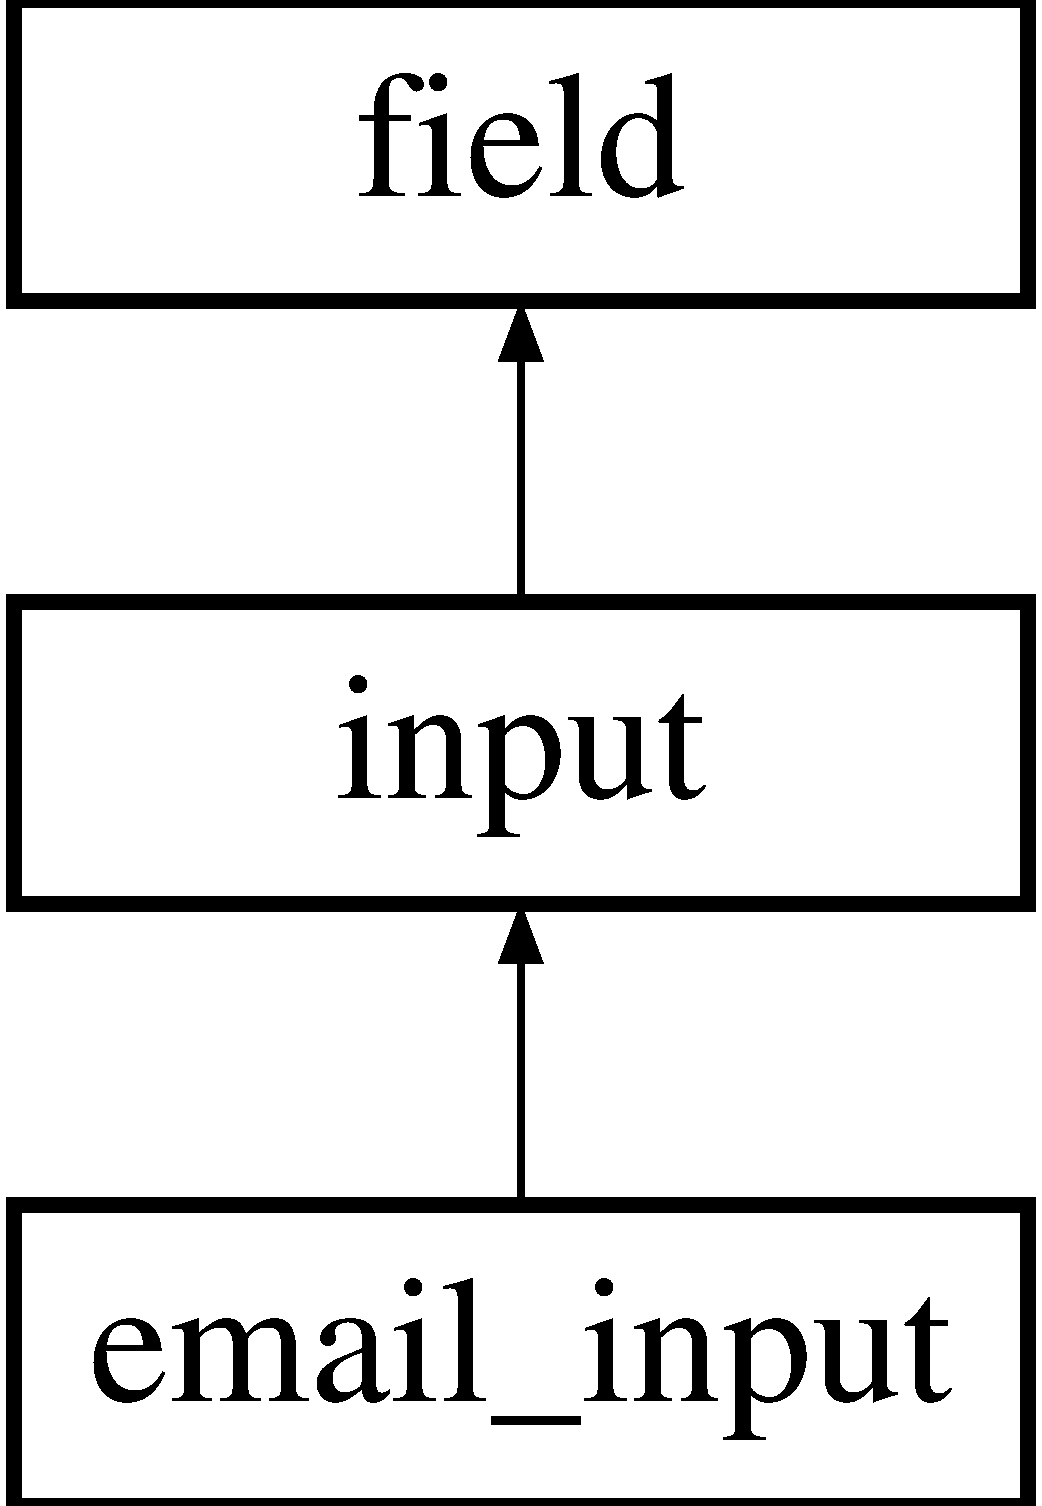
\includegraphics[height=3.000000cm]{classemail__input}
\end{center}
\end{figure}
\subsubsection*{Public Member Functions}
\begin{DoxyCompactItemize}
\item 
\hypertarget{classemail__input_ad0fcf81fbddaed253573fe659c84c9ab}{{\bfseries \-\_\-\-\_\-construct} (\$label\-\_\-text, \$name, \$value, \$required=false, \$maxlength= '', \$pattern= '', \$placeholder= '', \$sanity\-\_\-func=null, \$valid\-\_\-func=null)}\label{classemail__input_ad0fcf81fbddaed253573fe659c84c9ab}

\end{DoxyCompactItemize}
\subsubsection*{Additional Inherited Members}


The documentation for this class was generated from the following file\-:\begin{DoxyCompactItemize}
\item 
\hyperlink{extended__inputs_8inc_8php}{extended\-\_\-inputs.\-inc.\-php}\end{DoxyCompactItemize}

\hypertarget{classevent}{\subsection{event Class Reference}
\label{classevent}\index{event@{event}}
}


This describes an event in the observer pattern to pass information between the observable and observer.  


\subsubsection*{Public Member Functions}
\begin{DoxyCompactItemize}
\item 
\hypertarget{classevent_aef1a1991f2fdcbcfdba51b88e63a86fb}{{\bfseries event} (\&\$subject, \$event\-\_\-type, \&\$parameters=null)}\label{classevent_aef1a1991f2fdcbcfdba51b88e63a86fb}

\end{DoxyCompactItemize}
\subsubsection*{Public Attributes}
\begin{DoxyCompactItemize}
\item 
\hypertarget{classevent_a06fb7639aadb82d77ab0bee2cbdddcf7}{{\bfseries \$subject}}\label{classevent_a06fb7639aadb82d77ab0bee2cbdddcf7}

\item 
\hypertarget{classevent_ac6fc9038510c56f7d6c5c57d248b70db}{{\bfseries \$event\-\_\-type}}\label{classevent_ac6fc9038510c56f7d6c5c57d248b70db}

\item 
\hypertarget{classevent_a0759049c8b1681ce7337109ca9eac02d}{{\bfseries \$parameters}}\label{classevent_a0759049c8b1681ce7337109ca9eac02d}

\end{DoxyCompactItemize}


\subsubsection{Detailed Description}
This describes an event in the observer pattern to pass information between the observable and observer. 

The documentation for this class was generated from the following file\-:\begin{DoxyCompactItemize}
\item 
\hyperlink{event_8inc_8php}{event.\-inc.\-php}\end{DoxyCompactItemize}

\hypertarget{interfacefield}{\subsection{field Interface Reference}
\label{interfacefield}\index{field@{field}}
}
Inheritance diagram for field\-:\begin{figure}[H]
\begin{center}
\leavevmode
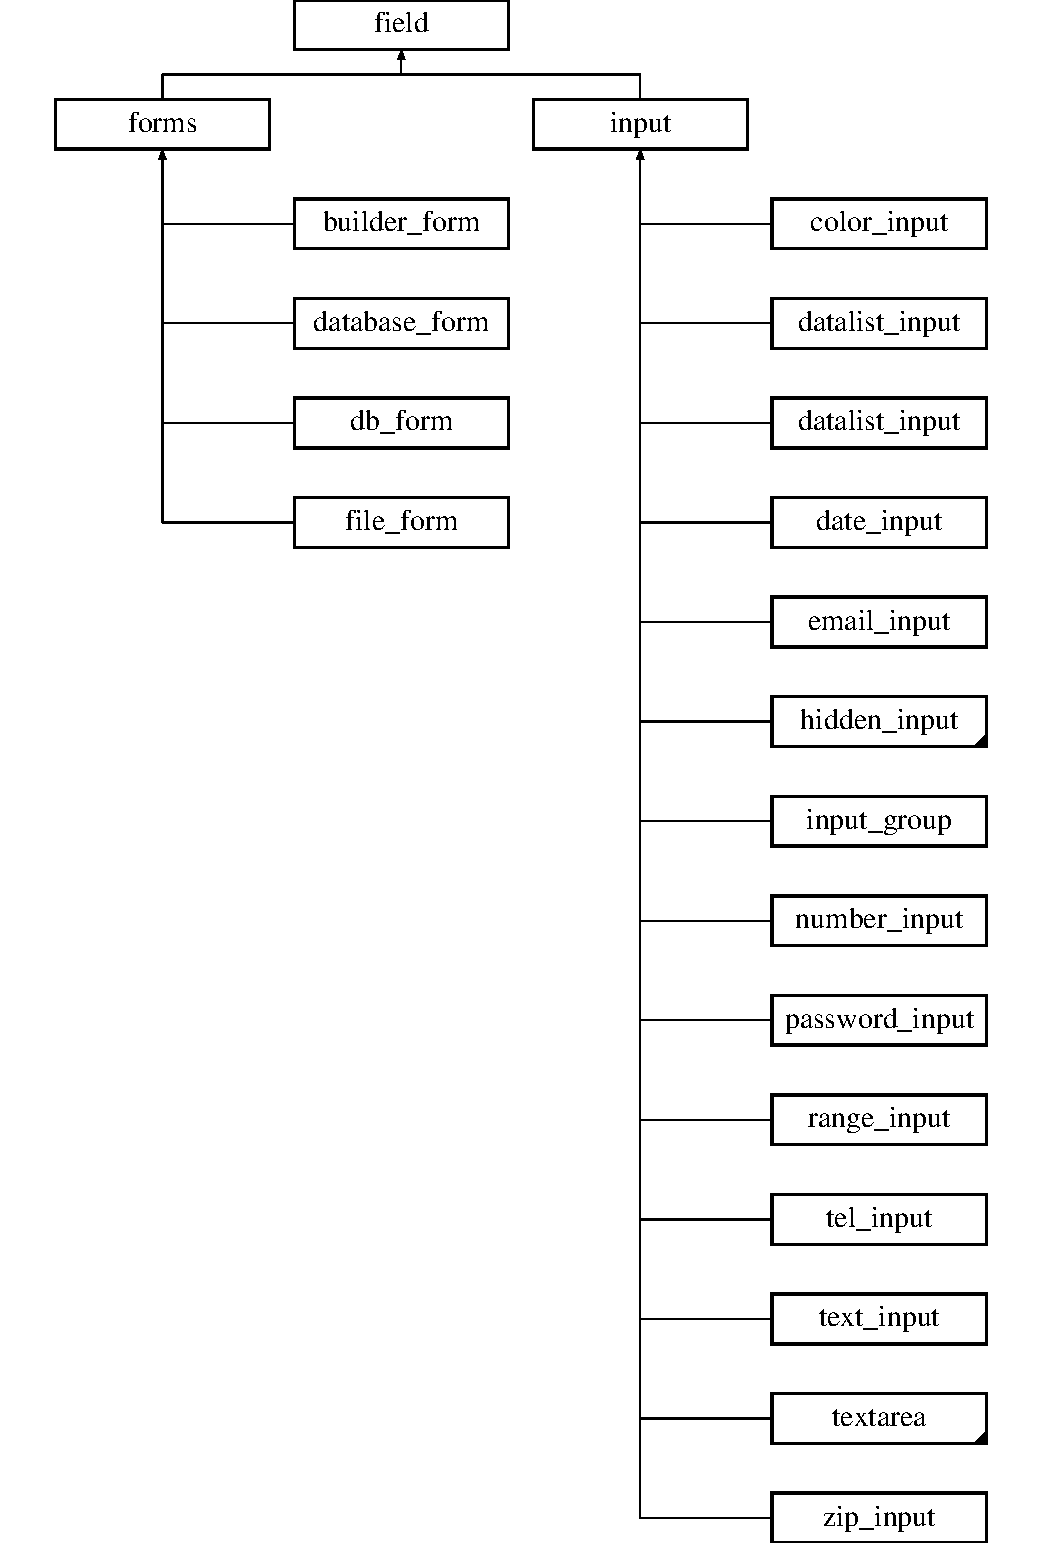
\includegraphics[height=12.000000cm]{interfacefield}
\end{center}
\end{figure}
\subsubsection*{Public Member Functions}
\begin{DoxyCompactItemize}
\item 
\hyperlink{interfacefield_a54958a09bc0dcd947d611b14741c5996}{values} (\$values)
\begin{DoxyCompactList}\small\item\em Takes an assoicated array of values and assigns the values to input fileds, and the id of this form. \end{DoxyCompactList}\item 
\hyperlink{interfacefield_a1b51c4b8b01f77a26eda359e1fc0fb4c}{form} (\$errors)
\begin{DoxyCompactList}\small\item\em Creates H\-T\-M\-L output of a form or form part (input) from this field. \end{DoxyCompactList}\item 
\hyperlink{interfacefield_a352b92f9e8dce69191bad79bdc5d972b}{validate} (\$errors)
\begin{DoxyCompactList}\small\item\em Validate the value(s) of this field, and append any errors onto the passed array. \end{DoxyCompactList}\item 
\hyperlink{interfacefield_a3ed132df10731b5ebe33acc44ac03c85}{sanitize} ()
\begin{DoxyCompactList}\small\item\em This function should sanitize the form for display and/or storage into a database. \end{DoxyCompactList}\item 
\hyperlink{interfacefield_a6a8bbd656a0e7cab2604f6df859bb60a}{display} ()
\begin{DoxyCompactList}\small\item\em Display the key value pairing for this object as a table. \end{DoxyCompactList}\item 
\hyperlink{interfacefield_a5e8d3e49ab5fba3956b7a297535806dc}{display\-\_\-text} ()
\begin{DoxyCompactList}\small\item\em Display the key value pairing for this object int text format. \end{DoxyCompactList}\end{DoxyCompactItemize}


\subsubsection{Member Function Documentation}
\hypertarget{interfacefield_a6a8bbd656a0e7cab2604f6df859bb60a}{\index{field@{field}!display@{display}}
\index{display@{display}!field@{field}}
\paragraph[{display}]{\setlength{\rightskip}{0pt plus 5cm}field\-::display (
\begin{DoxyParamCaption}
{}
\end{DoxyParamCaption}
)}}\label{interfacefield_a6a8bbd656a0e7cab2604f6df859bb60a}


Display the key value pairing for this object as a table. 

\begin{DoxyReturn}{Returns}
the H\-T\-M\-L representation of the field 
\end{DoxyReturn}


Implemented in \hyperlink{classdatalist__input_a6f94bf1247bd5da6f79c864b18073ed5}{datalist\-\_\-input}, \hyperlink{classinput_a993053ef011cade1db0ceaccb1f4da53}{input}, \hyperlink{classforms_abbb54cc0731f483777e6baa39f9fe494}{forms}, \hyperlink{classinput__group_a91e1b3cab54b81c21ab5f88a2f4f5c6a}{input\-\_\-group}, and \hyperlink{classhidden__input_a069e47104ea4bd965718c114013fa96f}{hidden\-\_\-input}.

\hypertarget{interfacefield_a5e8d3e49ab5fba3956b7a297535806dc}{\index{field@{field}!display\-\_\-text@{display\-\_\-text}}
\index{display\-\_\-text@{display\-\_\-text}!field@{field}}
\paragraph[{display\-\_\-text}]{\setlength{\rightskip}{0pt plus 5cm}field\-::display\-\_\-text (
\begin{DoxyParamCaption}
{}
\end{DoxyParamCaption}
)}}\label{interfacefield_a5e8d3e49ab5fba3956b7a297535806dc}


Display the key value pairing for this object int text format. 

\begin{DoxyReturn}{Returns}
the text representation of the field 
\end{DoxyReturn}


Implemented in \hyperlink{classinput_a344058a20cc48c9fe170b3b59905a53b}{input}, \hyperlink{classforms_ad78a6f47ecded8987dda90468dbb8f77}{forms}, and \hyperlink{classinput__group_aac74288da2e6c962dc507ccaa1f8f450}{input\-\_\-group}.

\hypertarget{interfacefield_a1b51c4b8b01f77a26eda359e1fc0fb4c}{\index{field@{field}!form@{form}}
\index{form@{form}!field@{field}}
\paragraph[{form}]{\setlength{\rightskip}{0pt plus 5cm}field\-::form (
\begin{DoxyParamCaption}
\item[{}]{\$errors}
\end{DoxyParamCaption}
)}}\label{interfacefield_a1b51c4b8b01f77a26eda359e1fc0fb4c}


Creates H\-T\-M\-L output of a form or form part (input) from this field. 


\begin{DoxyParams}[1]{Parameters}
array & {\em \$errors} & The errors that have been found, should be used to add error styles or display error messages. \\
\hline
\end{DoxyParams}
\begin{DoxyReturn}{Returns}
an associated array with two element 'html' =$>$ the H\-T\-M\-L of this object 'js' =$>$ the Javascript of this object 
\end{DoxyReturn}


Implemented in \hyperlink{classdatalist__input_aba53bff8ed66c85b97ce1ff23bfc15ec}{datalist\-\_\-input}, \hyperlink{classbuilder__form_a13989dd465615470a1145b401c672fcb}{builder\-\_\-form}, \hyperlink{classrange__input_a84223d881e2c9279e6ca69c4957bf53e}{range\-\_\-input}, \hyperlink{classinput_a83b663057f1d0f61768bc12c5a55f25c}{input}, \hyperlink{classforms_aca4fdeecf56bc5796f628a477f9ce629}{forms}, \hyperlink{classinput__group_a67f5d8e4ac86e75313e8d0d8696b7b35}{input\-\_\-group}, \hyperlink{classtextarea_a3e3d02a7c0ff76c86f6b987e1193ca6a}{textarea}, \hyperlink{classhidden__input_ab20546aae2284c4b1475854d0326e2e3}{hidden\-\_\-input}, and \hyperlink{classtexteditor_a129b929db008ec11f4a683f542787c74}{texteditor}.

\hypertarget{interfacefield_a3ed132df10731b5ebe33acc44ac03c85}{\index{field@{field}!sanitize@{sanitize}}
\index{sanitize@{sanitize}!field@{field}}
\paragraph[{sanitize}]{\setlength{\rightskip}{0pt plus 5cm}field\-::sanitize (
\begin{DoxyParamCaption}
{}
\end{DoxyParamCaption}
)}}\label{interfacefield_a3ed132df10731b5ebe33acc44ac03c85}


This function should sanitize the form for display and/or storage into a database. 

\begin{DoxyPostcond}{Postcondition}
the field's value should be considered 'safe'. 
\end{DoxyPostcond}


Implemented in \hyperlink{classdatalist__input_a52e50cc544ff141a03c2fc65bfdaf9ea}{datalist\-\_\-input}, \hyperlink{classinput_ab8456d2b5a929801af6fe0b36afd458c}{input}, \hyperlink{classinput__group_a4f0f7f8aeb74550c99114f28dca449cb}{input\-\_\-group}, and \hyperlink{classforms_a2494aca1309491b0ba423e233f4210b3}{forms}.

\hypertarget{interfacefield_a352b92f9e8dce69191bad79bdc5d972b}{\index{field@{field}!validate@{validate}}
\index{validate@{validate}!field@{field}}
\paragraph[{validate}]{\setlength{\rightskip}{0pt plus 5cm}field\-::validate (
\begin{DoxyParamCaption}
\item[{}]{\$errors}
\end{DoxyParamCaption}
)}}\label{interfacefield_a352b92f9e8dce69191bad79bdc5d972b}


Validate the value(s) of this field, and append any errors onto the passed array. 


\begin{DoxyParams}[1]{Parameters}
array & {\em \$errors} & An array of errors already encountered (optional). \\
\hline
\end{DoxyParams}
\begin{DoxyReturn}{Returns}
The passed array with any added errors. 
\end{DoxyReturn}


Implemented in \hyperlink{classdatalist__input_ab2827973f443100315d378d4a97b9516}{datalist\-\_\-input}, \hyperlink{classinput_aaf4ed91e7abbc20e2396a4b07dbd031a}{input}, \hyperlink{classforms_a80d7d5c6d738b6f42cfbb258b3c3a3d1}{forms}, and \hyperlink{classinput__group_ae0461a6034effccc3ca6bf34b6539cdd}{input\-\_\-group}.

\hypertarget{interfacefield_a54958a09bc0dcd947d611b14741c5996}{\index{field@{field}!values@{values}}
\index{values@{values}!field@{field}}
\paragraph[{values}]{\setlength{\rightskip}{0pt plus 5cm}field\-::values (
\begin{DoxyParamCaption}
\item[{}]{\$values}
\end{DoxyParamCaption}
)}}\label{interfacefield_a54958a09bc0dcd947d611b14741c5996}


Takes an assoicated array of values and assigns the values to input fileds, and the id of this form. 


\begin{DoxyParams}[1]{Parameters}
array & {\em \$values} & an associated array of values. Ignores values of keys that aren't fields in this form. \\
\hline
\end{DoxyParams}


Implemented in \hyperlink{classinput_a78f0cd122c69a6f62875152c0cfc9bc2}{input}, and \hyperlink{classforms_ad66e3f3a4d5332bbd15e53680930d786}{forms}.



The documentation for this interface was generated from the following file\-:\begin{DoxyCompactItemize}
\item 
\hyperlink{field_8inc_8php}{field.\-inc.\-php}\end{DoxyCompactItemize}

\hypertarget{classfile__form}{\subsection{file\-\_\-form Class Reference}
\label{classfile__form}\index{file\-\_\-form@{file\-\_\-form}}
}


This class represents an H\-T\-M\-L form, it's values, how it is validated and allows to read/write form data to serialized files.  


Inheritance diagram for file\-\_\-form\-:\begin{figure}[H]
\begin{center}
\leavevmode
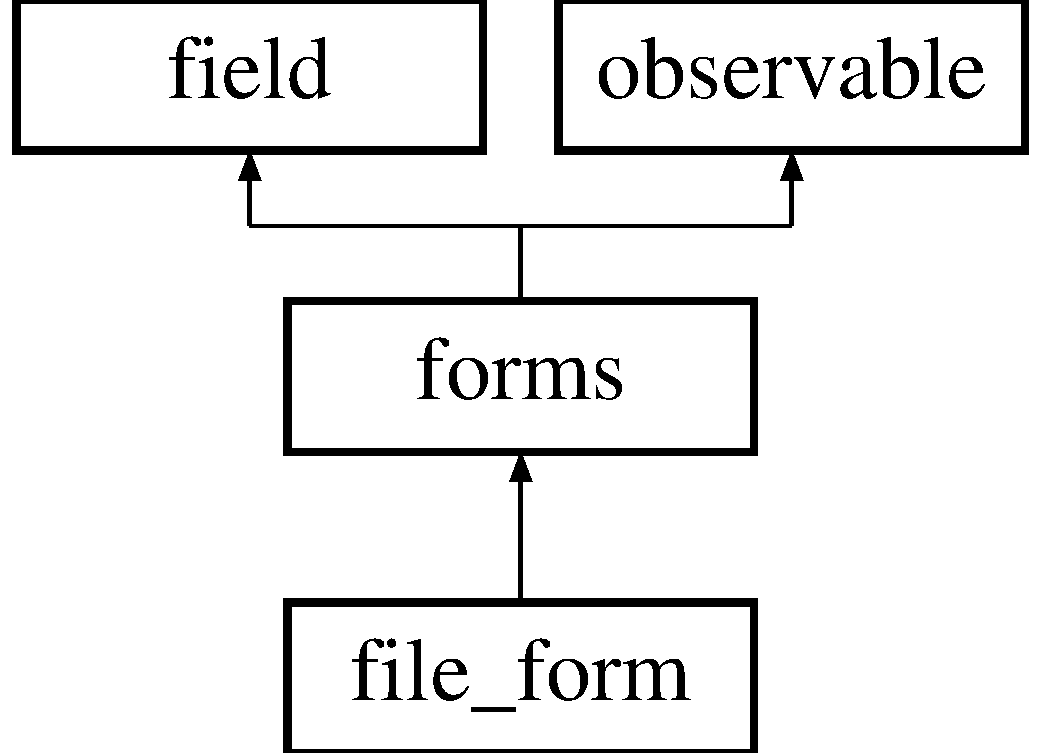
\includegraphics[height=3.000000cm]{classfile__form}
\end{center}
\end{figure}
\subsubsection*{Public Member Functions}
\begin{DoxyCompactItemize}
\item 
\hyperlink{classfile__form_a242c4711e97a3a9062ecbc4dfce8d2e0}{serialize\-\_\-data} ()
\begin{DoxyCompactList}\small\item\em Serializes form values for storage in variable, cookie or file. \end{DoxyCompactList}\item 
\hyperlink{classfile__form_a8b8ee5ff11a467aa1411355604c40904}{deserialize\-\_\-data} (\$s)
\begin{DoxyCompactList}\small\item\em Unserializes a string, and assigns the values to the field. \end{DoxyCompactList}\item 
\hyperlink{classfile__form_a29009ed5d4695a9298f167b17641ae1f}{save} ()
\begin{DoxyCompactList}\small\item\em Saves form data out to disk as serialized associated array. \end{DoxyCompactList}\item 
\hyperlink{classfile__form_a17b09200249a2b5c41261a19693dada8}{create} ()
\begin{DoxyCompactList}\small\item\em Creates a file from this form data. \end{DoxyCompactList}\item 
\hyperlink{classfile__form_ab7dce3d792551f836f20948fa9c8ef13}{read} ()
\begin{DoxyCompactList}\small\item\em Reads the values back into. \end{DoxyCompactList}\item 
\hyperlink{classfile__form_ad9573af92f2b4758204df70c01335f2e}{update} ()
\begin{DoxyCompactList}\small\item\em Updates the disk copy of this form. \end{DoxyCompactList}\item 
\hyperlink{classfile__form_aacbb6b50c48c05a74dd26e8abaee749a}{delete} ()
\begin{DoxyCompactList}\small\item\em Deletes the saved file containg this form. \end{DoxyCompactList}\end{DoxyCompactItemize}
\subsubsection*{Additional Inherited Members}


\subsubsection{Detailed Description}
This class represents an H\-T\-M\-L form, it's values, how it is validated and allows to read/write form data to serialized files. 

\subsubsection{Member Function Documentation}
\hypertarget{classfile__form_a17b09200249a2b5c41261a19693dada8}{\index{file\-\_\-form@{file\-\_\-form}!create@{create}}
\index{create@{create}!file_form@{file\-\_\-form}}
\paragraph[{create}]{\setlength{\rightskip}{0pt plus 5cm}file\-\_\-form\-::create (
\begin{DoxyParamCaption}
{}
\end{DoxyParamCaption}
)}}\label{classfile__form_a17b09200249a2b5c41261a19693dada8}


Creates a file from this form data. 

\begin{DoxySeeAlso}{See Also}
\hyperlink{classfile__form_a29009ed5d4695a9298f167b17641ae1f}{file\-\_\-form\-::save()} 
\end{DoxySeeAlso}
\begin{DoxyRefDesc}{Todo}
\item[\hyperlink{todo__todo000007}{Todo}]get new id 

locking. \end{DoxyRefDesc}
\hypertarget{classfile__form_aacbb6b50c48c05a74dd26e8abaee749a}{\index{file\-\_\-form@{file\-\_\-form}!delete@{delete}}
\index{delete@{delete}!file_form@{file\-\_\-form}}
\paragraph[{delete}]{\setlength{\rightskip}{0pt plus 5cm}file\-\_\-form\-::delete (
\begin{DoxyParamCaption}
{}
\end{DoxyParamCaption}
)}}\label{classfile__form_aacbb6b50c48c05a74dd26e8abaee749a}


Deletes the saved file containg this form. 

\begin{DoxyReturn}{Returns}
true if successful otherwise false. 
\end{DoxyReturn}
\begin{DoxyRefDesc}{Todo}
\item[\hyperlink{todo__todo000010}{Todo}]locking. \end{DoxyRefDesc}
\hypertarget{classfile__form_a8b8ee5ff11a467aa1411355604c40904}{\index{file\-\_\-form@{file\-\_\-form}!deserialize\-\_\-data@{deserialize\-\_\-data}}
\index{deserialize\-\_\-data@{deserialize\-\_\-data}!file_form@{file\-\_\-form}}
\paragraph[{deserialize\-\_\-data}]{\setlength{\rightskip}{0pt plus 5cm}file\-\_\-form\-::deserialize\-\_\-data (
\begin{DoxyParamCaption}
\item[{}]{\$s}
\end{DoxyParamCaption}
)}}\label{classfile__form_a8b8ee5ff11a467aa1411355604c40904}


Unserializes a string, and assigns the values to the field. 


\begin{DoxyParams}{Parameters}
{\em \$s} & the serialized version of an associated array. Ignores values whose keys are not fields of this form. \\
\hline
\end{DoxyParams}
\begin{DoxySeeAlso}{See Also}
\hyperlink{classfile__form_a242c4711e97a3a9062ecbc4dfce8d2e0}{file\-\_\-form\-::serialize\-\_\-data()} 

\hyperlink{classforms_ad66e3f3a4d5332bbd15e53680930d786}{forms\-::values()} 
\end{DoxySeeAlso}
\hypertarget{classfile__form_ab7dce3d792551f836f20948fa9c8ef13}{\index{file\-\_\-form@{file\-\_\-form}!read@{read}}
\index{read@{read}!file_form@{file\-\_\-form}}
\paragraph[{read}]{\setlength{\rightskip}{0pt plus 5cm}file\-\_\-form\-::read (
\begin{DoxyParamCaption}
{}
\end{DoxyParamCaption}
)}}\label{classfile__form_ab7dce3d792551f836f20948fa9c8ef13}


Reads the values back into. 

\begin{DoxySeeAlso}{See Also}
\hyperlink{classfile__form_a8b8ee5ff11a467aa1411355604c40904}{file\-\_\-form\-::deserialize\-\_\-data()} 
\end{DoxySeeAlso}
\begin{DoxyRefDesc}{Todo}
\item[\hyperlink{todo__todo000008}{Todo}]locking. \end{DoxyRefDesc}
\hypertarget{classfile__form_a29009ed5d4695a9298f167b17641ae1f}{\index{file\-\_\-form@{file\-\_\-form}!save@{save}}
\index{save@{save}!file_form@{file\-\_\-form}}
\paragraph[{save}]{\setlength{\rightskip}{0pt plus 5cm}file\-\_\-form\-::save (
\begin{DoxyParamCaption}
{}
\end{DoxyParamCaption}
)}}\label{classfile__form_a29009ed5d4695a9298f167b17641ae1f}


Saves form data out to disk as serialized associated array. 

File is saved to $<$form name$>$=\char`\"{}\char`\"{}$>$.data/$<$id$>$.frm \begin{DoxySeeAlso}{See Also}
\hyperlink{classfile__form_a242c4711e97a3a9062ecbc4dfce8d2e0}{file\-\_\-form\-::serialize\-\_\-data} 
\end{DoxySeeAlso}
\hypertarget{classfile__form_a242c4711e97a3a9062ecbc4dfce8d2e0}{\index{file\-\_\-form@{file\-\_\-form}!serialize\-\_\-data@{serialize\-\_\-data}}
\index{serialize\-\_\-data@{serialize\-\_\-data}!file_form@{file\-\_\-form}}
\paragraph[{serialize\-\_\-data}]{\setlength{\rightskip}{0pt plus 5cm}file\-\_\-form\-::serialize\-\_\-data (
\begin{DoxyParamCaption}
{}
\end{DoxyParamCaption}
)}}\label{classfile__form_a242c4711e97a3a9062ecbc4dfce8d2e0}


Serializes form values for storage in variable, cookie or file. 

\begin{DoxyReturn}{Returns}
string of serialized array of values. 
\end{DoxyReturn}
\begin{DoxySeeAlso}{See Also}
\hyperlink{classfile__form_a8b8ee5ff11a467aa1411355604c40904}{file\-\_\-form\-::deserialize\-\_\-data()} 
\end{DoxySeeAlso}
\hypertarget{classfile__form_ad9573af92f2b4758204df70c01335f2e}{\index{file\-\_\-form@{file\-\_\-form}!update@{update}}
\index{update@{update}!file_form@{file\-\_\-form}}
\paragraph[{update}]{\setlength{\rightskip}{0pt plus 5cm}file\-\_\-form\-::update (
\begin{DoxyParamCaption}
{}
\end{DoxyParamCaption}
)}}\label{classfile__form_ad9573af92f2b4758204df70c01335f2e}


Updates the disk copy of this form. 

\begin{DoxySeeAlso}{See Also}
\hyperlink{classfile__form_a29009ed5d4695a9298f167b17641ae1f}{file\-\_\-form\-::save()} 
\end{DoxySeeAlso}
\begin{DoxyRefDesc}{Todo}
\item[\hyperlink{todo__todo000009}{Todo}]locking. \end{DoxyRefDesc}


The documentation for this class was generated from the following file\-:\begin{DoxyCompactItemize}
\item 
\hyperlink{file__form_8inc_8php}{file\-\_\-form.\-inc.\-php}\end{DoxyCompactItemize}

\hypertarget{classforms}{\subsection{forms Class Reference}
\label{classforms}\index{forms@{forms}}
}


This class describes an H\-T\-M\-L form, containing a collection of inputs, and does mass validation and sanitization on them.  


Inheritance diagram for forms\-:\begin{figure}[H]
\begin{center}
\leavevmode
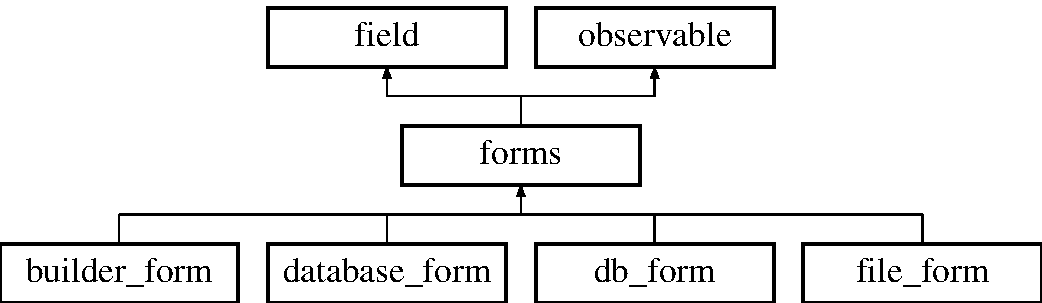
\includegraphics[height=3.000000cm]{classforms}
\end{center}
\end{figure}
\subsubsection*{Public Member Functions}
\begin{DoxyCompactItemize}
\item 
\hyperlink{classforms_a89ff17c0b763f0fd16abbe6ebd2dbe96}{forms} (\$name, \$fields, \$id='', \$pre='')
\begin{DoxyCompactList}\small\item\em Constructor for form class. \end{DoxyCompactList}\item 
\hyperlink{classforms_aca4fdeecf56bc5796f628a477f9ce629}{form} (\$errors=array())
\begin{DoxyCompactList}\small\item\em Returns the H\-T\-M\-L and Java\-Script for this form. \end{DoxyCompactList}\item 
\hyperlink{classforms_a2494aca1309491b0ba423e233f4210b3}{sanitize} ()
\begin{DoxyCompactList}\small\item\em Sanitize field values to help protect against H\-T\-M\-L, S\-Q\-L, P\-H\-P or other injection. \end{DoxyCompactList}\item 
\hyperlink{classforms_abbb54cc0731f483777e6baa39f9fe494}{display} ()
\begin{DoxyCompactList}\small\item\em Display this form's name values pairs. \end{DoxyCompactList}\item 
\hyperlink{classforms_ad78a6f47ecded8987dda90468dbb8f77}{display\-\_\-text} ()
\begin{DoxyCompactList}\small\item\em Display this form's name values pairs. \end{DoxyCompactList}\item 
\hyperlink{classforms_a80d7d5c6d738b6f42cfbb258b3c3a3d1}{validate} (\$errors=array())
\begin{DoxyCompactList}\small\item\em Validates the values of the input of the form. \end{DoxyCompactList}\item 
\hyperlink{classforms_ad85afb257cfdcf8834590774fd9ef357}{add\-\_\-field} (\hyperlink{interfacefield}{field} \$f)
\begin{DoxyCompactList}\small\item\em Adds a field to this form. \end{DoxyCompactList}\item 
\hyperlink{classforms_ad66e3f3a4d5332bbd15e53680930d786}{values} (\$values)
\begin{DoxyCompactList}\small\item\em Takes an assoicated array of values and assigns the values to input fileds, and the id of this form. \end{DoxyCompactList}\item 
\hyperlink{classforms_a82bc2b5e603ecd535f362c3dfdcae96e}{notify} (\$\hyperlink{classevent}{event})
\begin{DoxyCompactList}\small\item\em Notify observers an \$event has taken place. \end{DoxyCompactList}\item 
\hyperlink{classforms_a6c88ab2728699cc06ba8110b1f5aacbc}{add\-\_\-observer} (\$ob)
\begin{DoxyCompactList}\small\item\em Add an observer to watch \$this object. \end{DoxyCompactList}\item 
\hyperlink{classforms_af5c72c905909819f8824958c2faa015d}{remove\-\_\-observer} (\$ob)
\begin{DoxyCompactList}\small\item\em Remove an observer of \$this object. \end{DoxyCompactList}\end{DoxyCompactItemize}
\subsubsection*{Public Attributes}
\begin{DoxyCompactItemize}
\item 
\hypertarget{classforms_aa84609327e0f9bdf2ba799c8cd2268fd}{{\bfseries \$name}}\label{classforms_aa84609327e0f9bdf2ba799c8cd2268fd}

\item 
\hypertarget{classforms_a43144384180122ef4434845671a45e4c}{{\bfseries \$id}}\label{classforms_a43144384180122ef4434845671a45e4c}

\item 
\hypertarget{classforms_a55665dfe896e78efdfd33a650f6e2d7c}{{\bfseries \$pre}}\label{classforms_a55665dfe896e78efdfd33a650f6e2d7c}

\item 
\hypertarget{classforms_a4df40ac2adbfb971665ab358fc8954b5}{{\bfseries \$fields}}\label{classforms_a4df40ac2adbfb971665ab358fc8954b5}

\item 
\hypertarget{classforms_aebf137dbe732b7eee3786e3b1ec24535}{{\bfseries \$observers}}\label{classforms_aebf137dbe732b7eee3786e3b1ec24535}

\end{DoxyCompactItemize}


\subsubsection{Detailed Description}
This class describes an H\-T\-M\-L form, containing a collection of inputs, and does mass validation and sanitization on them. 

\subsubsection{Member Function Documentation}
\hypertarget{classforms_ad85afb257cfdcf8834590774fd9ef357}{\index{forms@{forms}!add\-\_\-field@{add\-\_\-field}}
\index{add\-\_\-field@{add\-\_\-field}!forms@{forms}}
\paragraph[{add\-\_\-field}]{\setlength{\rightskip}{0pt plus 5cm}forms\-::add\-\_\-field (
\begin{DoxyParamCaption}
\item[{{\bf field}}]{\$f}
\end{DoxyParamCaption}
)}}\label{classforms_ad85afb257cfdcf8834590774fd9ef357}


Adds a field to this form. 


\begin{DoxyParams}{Parameters}
{\em field} & input \$f The new input, Two fields cannot have the same name. \\
\hline
\end{DoxyParams}
\begin{DoxyReturn}{Returns}
true if field is added 
\end{DoxyReturn}
\hypertarget{classforms_a6c88ab2728699cc06ba8110b1f5aacbc}{\index{forms@{forms}!add\-\_\-observer@{add\-\_\-observer}}
\index{add\-\_\-observer@{add\-\_\-observer}!forms@{forms}}
\paragraph[{add\-\_\-observer}]{\setlength{\rightskip}{0pt plus 5cm}forms\-::add\-\_\-observer (
\begin{DoxyParamCaption}
\item[{}]{\$ob}
\end{DoxyParamCaption}
)}}\label{classforms_a6c88ab2728699cc06ba8110b1f5aacbc}


Add an observer to watch \$this object. 


\begin{DoxyParams}[1]{Parameters}
observer & {\em \$ob} & The object waiting for state change. \\
\hline
\end{DoxyParams}


Implements \hyperlink{interfaceobservable_aa4c1e85f5ec861411aa1d99ee0471082}{observable}.

\hypertarget{classforms_abbb54cc0731f483777e6baa39f9fe494}{\index{forms@{forms}!display@{display}}
\index{display@{display}!forms@{forms}}
\paragraph[{display}]{\setlength{\rightskip}{0pt plus 5cm}forms\-::display (
\begin{DoxyParamCaption}
{}
\end{DoxyParamCaption}
)}}\label{classforms_abbb54cc0731f483777e6baa39f9fe494}


Display this form's name values pairs. 

\begin{DoxyReturn}{Returns}
string containing an H\-T\-M\-L table of values. 
\end{DoxyReturn}


Implements \hyperlink{interfacefield_a6a8bbd656a0e7cab2604f6df859bb60a}{field}.

\hypertarget{classforms_ad78a6f47ecded8987dda90468dbb8f77}{\index{forms@{forms}!display\-\_\-text@{display\-\_\-text}}
\index{display\-\_\-text@{display\-\_\-text}!forms@{forms}}
\paragraph[{display\-\_\-text}]{\setlength{\rightskip}{0pt plus 5cm}forms\-::display\-\_\-text (
\begin{DoxyParamCaption}
{}
\end{DoxyParamCaption}
)}}\label{classforms_ad78a6f47ecded8987dda90468dbb8f77}


Display this form's name values pairs. 

\begin{DoxyReturn}{Returns}
string containing an txt table of values. 
\end{DoxyReturn}


Implements \hyperlink{interfacefield_a5e8d3e49ab5fba3956b7a297535806dc}{field}.

\hypertarget{classforms_aca4fdeecf56bc5796f628a477f9ce629}{\index{forms@{forms}!form@{form}}
\index{form@{form}!forms@{forms}}
\paragraph[{form}]{\setlength{\rightskip}{0pt plus 5cm}forms\-::form (
\begin{DoxyParamCaption}
\item[{}]{\$errors = {\ttfamily array()}}
\end{DoxyParamCaption}
)}}\label{classforms_aca4fdeecf56bc5796f628a477f9ce629}


Returns the H\-T\-M\-L and Java\-Script for this form. 


\begin{DoxyParams}{Parameters}
{\em \$errors} & an array of errors, used to add class to fields which have an error \\
\hline
\end{DoxyParams}
\begin{DoxyReturn}{Returns}
array of strings with 'html' =$>$ the H\-T\-M\-L of the form, and 'js' =$>$ any J\-S the form elements may need 
\end{DoxyReturn}
\begin{DoxySeeAlso}{See Also}
\hyperlink{classinput_a83b663057f1d0f61768bc12c5a55f25c}{input\-::form()} 
\end{DoxySeeAlso}


Implements \hyperlink{interfacefield_a1b51c4b8b01f77a26eda359e1fc0fb4c}{field}.

\hypertarget{classforms_a89ff17c0b763f0fd16abbe6ebd2dbe96}{\index{forms@{forms}!forms@{forms}}
\index{forms@{forms}!forms@{forms}}
\paragraph[{forms}]{\setlength{\rightskip}{0pt plus 5cm}forms\-::forms (
\begin{DoxyParamCaption}
\item[{}]{\$name, }
\item[{}]{\$fields, }
\item[{}]{\$id = {\ttfamily ''}, }
\item[{}]{\$pre = {\ttfamily ''}}
\end{DoxyParamCaption}
)}}\label{classforms_a89ff17c0b763f0fd16abbe6ebd2dbe96}


Constructor for form class. 


\begin{DoxyParams}[1]{Parameters}
string & {\em \$name} & The name of form. \\
\hline
array & {\em \$fields} & The fields of the form, as an array of input objects. \\
\hline
\end{DoxyParams}
\hypertarget{classforms_a82bc2b5e603ecd535f362c3dfdcae96e}{\index{forms@{forms}!notify@{notify}}
\index{notify@{notify}!forms@{forms}}
\paragraph[{notify}]{\setlength{\rightskip}{0pt plus 5cm}forms\-::notify (
\begin{DoxyParamCaption}
\item[{}]{\$event}
\end{DoxyParamCaption}
)}}\label{classforms_a82bc2b5e603ecd535f362c3dfdcae96e}


Notify observers an \$event has taken place. 


\begin{DoxyParams}{Parameters}
{\em \$event} & The event that's occured. \\
\hline
\end{DoxyParams}


Implements \hyperlink{interfaceobservable_aa4d6d161d4154a3525e93f6c051e1914}{observable}.

\hypertarget{classforms_af5c72c905909819f8824958c2faa015d}{\index{forms@{forms}!remove\-\_\-observer@{remove\-\_\-observer}}
\index{remove\-\_\-observer@{remove\-\_\-observer}!forms@{forms}}
\paragraph[{remove\-\_\-observer}]{\setlength{\rightskip}{0pt plus 5cm}forms\-::remove\-\_\-observer (
\begin{DoxyParamCaption}
\item[{}]{\$ob}
\end{DoxyParamCaption}
)}}\label{classforms_af5c72c905909819f8824958c2faa015d}


Remove an observer of \$this object. 


\begin{DoxyParams}[1]{Parameters}
observer & {\em \$ob} & The oberserver we want to remove. \\
\hline
\end{DoxyParams}
\begin{DoxyReturn}{Returns}
True if found and removed, false if not. 
\end{DoxyReturn}


Implements \hyperlink{interfaceobservable_aea49f4e7d1c3181031e50c15e0bfd9d4}{observable}.

\hypertarget{classforms_a2494aca1309491b0ba423e233f4210b3}{\index{forms@{forms}!sanitize@{sanitize}}
\index{sanitize@{sanitize}!forms@{forms}}
\paragraph[{sanitize}]{\setlength{\rightskip}{0pt plus 5cm}forms\-::sanitize (
\begin{DoxyParamCaption}
{}
\end{DoxyParamCaption}
)}}\label{classforms_a2494aca1309491b0ba423e233f4210b3}


Sanitize field values to help protect against H\-T\-M\-L, S\-Q\-L, P\-H\-P or other injection. 

\begin{DoxyReturn}{Returns}
bool true if form could be sanitized, returns false if input was too mangled to sanitize. 
\end{DoxyReturn}


Implements \hyperlink{interfacefield_a3ed132df10731b5ebe33acc44ac03c85}{field}.

\hypertarget{classforms_a80d7d5c6d738b6f42cfbb258b3c3a3d1}{\index{forms@{forms}!validate@{validate}}
\index{validate@{validate}!forms@{forms}}
\paragraph[{validate}]{\setlength{\rightskip}{0pt plus 5cm}forms\-::validate (
\begin{DoxyParamCaption}
\item[{}]{\$errors = {\ttfamily array()}}
\end{DoxyParamCaption}
)}}\label{classforms_a80d7d5c6d738b6f42cfbb258b3c3a3d1}


Validates the values of the input of the form. 


\begin{DoxyParams}{Parameters}
{\em \$errors} & an optional array to chain form validation with other inputs and forms. \\
\hline
\end{DoxyParams}
\begin{DoxyReturn}{Returns}
\$errors the passed array with new errors encountered. 
\end{DoxyReturn}


Implements \hyperlink{interfacefield_a352b92f9e8dce69191bad79bdc5d972b}{field}.

\hypertarget{classforms_ad66e3f3a4d5332bbd15e53680930d786}{\index{forms@{forms}!values@{values}}
\index{values@{values}!forms@{forms}}
\paragraph[{values}]{\setlength{\rightskip}{0pt plus 5cm}forms\-::values (
\begin{DoxyParamCaption}
\item[{}]{\$values}
\end{DoxyParamCaption}
)}}\label{classforms_ad66e3f3a4d5332bbd15e53680930d786}


Takes an assoicated array of values and assigns the values to input fileds, and the id of this form. 


\begin{DoxyParams}[1]{Parameters}
array & {\em \$values} & an associated array of values. Ignores values of keys that aren't fields in this form. \\
\hline
\end{DoxyParams}


Implements \hyperlink{interfacefield_a54958a09bc0dcd947d611b14741c5996}{field}.



The documentation for this class was generated from the following file\-:\begin{DoxyCompactItemize}
\item 
\hyperlink{forms_8inc_8php}{forms.\-inc.\-php}\end{DoxyCompactItemize}

\hypertarget{classfund__item}{\subsection{fund\-\_\-item Class Reference}
\label{classfund__item}\index{fund\-\_\-item@{fund\-\_\-item}}
}
\subsubsection*{Public Member Functions}
\begin{DoxyCompactItemize}
\item 
\hypertarget{classfund__item_af69090971e06f95d3111bc3929bbc7ed}{{\bfseries fund\-\_\-item} (\$pre= '', \$fund\-\_\-item\-\_\-id= '', \$pcard= '', \$tcard= '', \$cash= '')}\label{classfund__item_af69090971e06f95d3111bc3929bbc7ed}

\item 
\hypertarget{classfund__item_aa8628904b128c99427ffa76221c25dfe}{{\bfseries sanitize} ()}\label{classfund__item_aa8628904b128c99427ffa76221c25dfe}

\item 
\hypertarget{classfund__item_a2109568c112c06633edc9c37b5d86df1}{{\bfseries validate} (\$errors=array())}\label{classfund__item_a2109568c112c06633edc9c37b5d86df1}

\item 
\hypertarget{classfund__item_a4e39a4bb6a2e90742676ed85f962fb41}{{\bfseries form} (\$errors=array())}\label{classfund__item_a4e39a4bb6a2e90742676ed85f962fb41}

\item 
\hypertarget{classfund__item_a724d21d4ff770da7a292acb470889a5d}{{\bfseries create} ()}\label{classfund__item_a724d21d4ff770da7a292acb470889a5d}

\item 
\hypertarget{classfund__item_a1466fe9e207fbd60997abc95b166c029}{{\bfseries read} ()}\label{classfund__item_a1466fe9e207fbd60997abc95b166c029}

\item 
\hypertarget{classfund__item_a57e77343b1a2fe03ae2407372cf00a2b}{{\bfseries update} ()}\label{classfund__item_a57e77343b1a2fe03ae2407372cf00a2b}

\item 
\hypertarget{classfund__item_a25a1cda3c7b7ab89f212b9b07bec25b8}{{\bfseries delete} ()}\label{classfund__item_a25a1cda3c7b7ab89f212b9b07bec25b8}

\end{DoxyCompactItemize}
\subsubsection*{Public Attributes}
\begin{DoxyCompactItemize}
\item 
\hypertarget{classfund__item_abf08e6e8d8c218c4bbb8a3a1053fb2d5}{{\bfseries \$fund\-\_\-item\-\_\-id}}\label{classfund__item_abf08e6e8d8c218c4bbb8a3a1053fb2d5}

\item 
\hypertarget{classfund__item_abd6a959afb9a9bc1af2946bb71714d5a}{{\bfseries \$pcard}}\label{classfund__item_abd6a959afb9a9bc1af2946bb71714d5a}

\item 
\hypertarget{classfund__item_ab35ea22221cb19077b1e1133773fee59}{{\bfseries \$tcard}}\label{classfund__item_ab35ea22221cb19077b1e1133773fee59}

\item 
\hypertarget{classfund__item_aaa36cf70014063ae31fe6cb4990131c5}{{\bfseries \$cash}}\label{classfund__item_aaa36cf70014063ae31fe6cb4990131c5}

\item 
\hypertarget{classfund__item_aa1a2b7aa4da7927075185873e5559886}{{\bfseries \$pre}}\label{classfund__item_aa1a2b7aa4da7927075185873e5559886}

\end{DoxyCompactItemize}


The documentation for this class was generated from the following file\-:\begin{DoxyCompactItemize}
\item 
request.\-inc.\-php\end{DoxyCompactItemize}

\hypertarget{classfunding}{\subsection{funding Class Reference}
\label{classfunding}\index{funding@{funding}}
}
\subsubsection*{Public Member Functions}
\begin{DoxyCompactItemize}
\item 
\hypertarget{classfunding_a14ea2650bff671baf21ae1b11f0ec468}{{\bfseries funding} (\$pre= '', \$fund\-\_\-id= '', \$fund= '', \$org= '', \$program= '', account= '', amount= '')}\label{classfunding_a14ea2650bff671baf21ae1b11f0ec468}

\item 
\hypertarget{classfunding_a75ec9e0289af4245f07fcfaac057c32c}{{\bfseries sanitize} ()}\label{classfunding_a75ec9e0289af4245f07fcfaac057c32c}

\item 
\hypertarget{classfunding_aa8cafb705f2d48254a99f1689edccd90}{{\bfseries validate} (\$errors=array())}\label{classfunding_aa8cafb705f2d48254a99f1689edccd90}

\item 
\hypertarget{classfunding_a1687ae9406c7a5749b5fddd6e7c75b12}{{\bfseries form} (\$errors=array())}\label{classfunding_a1687ae9406c7a5749b5fddd6e7c75b12}

\item 
\hypertarget{classfunding_a389dbb80bf1f79480baf806e87a97e26}{{\bfseries create} ()}\label{classfunding_a389dbb80bf1f79480baf806e87a97e26}

\item 
\hypertarget{classfunding_ac4cc66b323f4dbacaeee42610ef27a01}{{\bfseries read} ()}\label{classfunding_ac4cc66b323f4dbacaeee42610ef27a01}

\item 
\hypertarget{classfunding_a53b8e2eb37bebccbb88e8225a913215f}{{\bfseries update} ()}\label{classfunding_a53b8e2eb37bebccbb88e8225a913215f}

\item 
\hypertarget{classfunding_aa38f3aa17354941e7316962d712ae9ba}{{\bfseries delete} ()}\label{classfunding_aa38f3aa17354941e7316962d712ae9ba}

\end{DoxyCompactItemize}
\subsubsection*{Public Attributes}
\begin{DoxyCompactItemize}
\item 
\hypertarget{classfunding_ad97cefcb5214a45322cf25a6bfad437a}{{\bfseries \$funding\-\_\-id}}\label{classfunding_ad97cefcb5214a45322cf25a6bfad437a}

\item 
\hypertarget{classfunding_a1f25e2e1e6844cae492cd4c8492c4eda}{{\bfseries \$fund}}\label{classfunding_a1f25e2e1e6844cae492cd4c8492c4eda}

\item 
\hypertarget{classfunding_aa47d01dfc738988a34dea159fd711aee}{{\bfseries \$org}}\label{classfunding_aa47d01dfc738988a34dea159fd711aee}

\item 
\hypertarget{classfunding_ab185734c844be5ced263fe1734db6a36}{{\bfseries \$program}}\label{classfunding_ab185734c844be5ced263fe1734db6a36}

\item 
\hypertarget{classfunding_aae462c12720de4ac6df8e695bf973e1b}{{\bfseries \$account}}\label{classfunding_aae462c12720de4ac6df8e695bf973e1b}

\item 
\hypertarget{classfunding_ae3aa61fa39c596b3cd5616aea5c6c208}{{\bfseries \$amount}}\label{classfunding_ae3aa61fa39c596b3cd5616aea5c6c208}

\item 
\hypertarget{classfunding_a8884b1589de04a51934cc1414bb3dd95}{{\bfseries \$pre}}\label{classfunding_a8884b1589de04a51934cc1414bb3dd95}

\end{DoxyCompactItemize}


The documentation for this class was generated from the following file\-:\begin{DoxyCompactItemize}
\item 
request.\-inc.\-php\end{DoxyCompactItemize}

\hypertarget{classget__input}{\subsection{get\-\_\-input Class Reference}
\label{classget__input}\index{get\-\_\-input@{get\-\_\-input}}
}


An \hyperlink{classhidden__input}{hidden\-\_\-input} that reads its value from the \$\-\_\-\-G\-E\-T global array on creation.  


Inheritance diagram for get\-\_\-input\-:\begin{figure}[H]
\begin{center}
\leavevmode
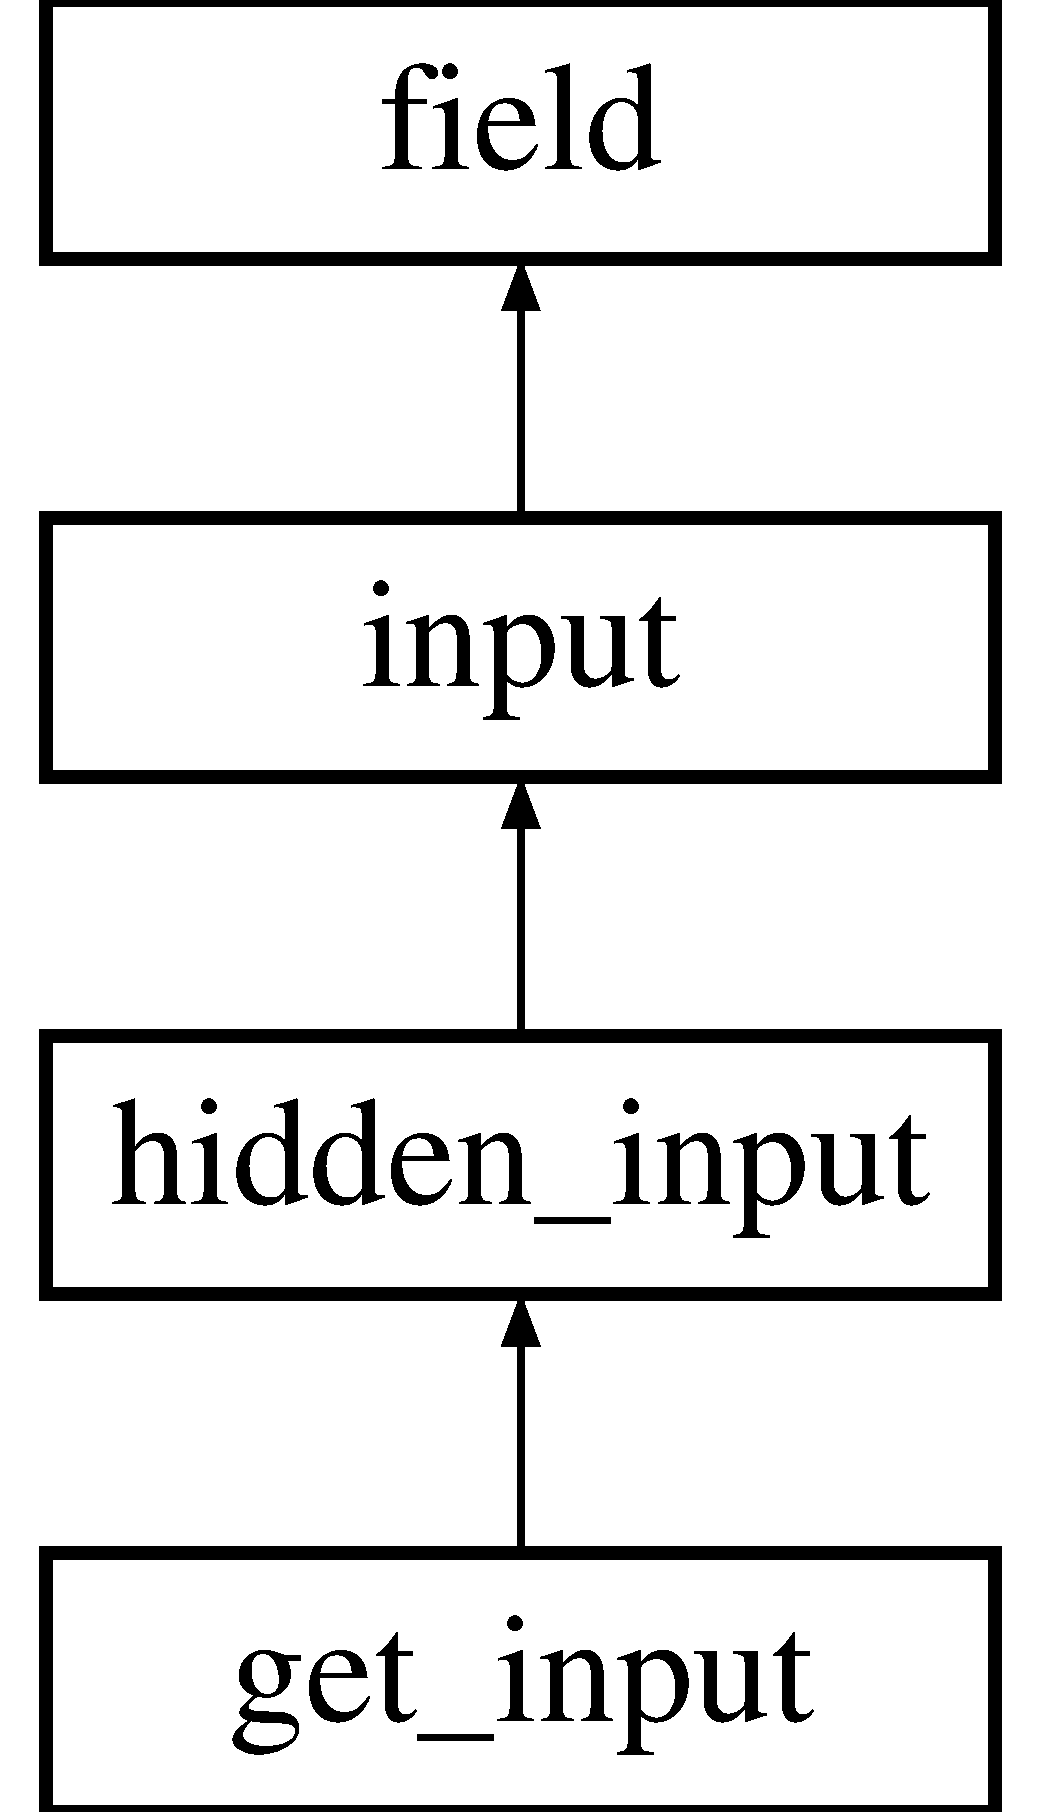
\includegraphics[height=4.000000cm]{classget__input}
\end{center}
\end{figure}
\subsubsection*{Public Member Functions}
\begin{DoxyCompactItemize}
\item 
\hyperlink{classget__input_a381a7271f72a0231a6a2c7a20f960410}{get\-\_\-input} (\$name, \$sanity\-\_\-func=null, \$valid\-\_\-func=null)
\begin{DoxyCompactList}\small\item\em Constructor. \end{DoxyCompactList}\end{DoxyCompactItemize}
\subsubsection*{Additional Inherited Members}


\subsubsection{Detailed Description}
An \hyperlink{classhidden__input}{hidden\-\_\-input} that reads its value from the \$\-\_\-\-G\-E\-T global array on creation. 

\subsubsection{Member Function Documentation}
\hypertarget{classget__input_a381a7271f72a0231a6a2c7a20f960410}{\index{get\-\_\-input@{get\-\_\-input}!get\-\_\-input@{get\-\_\-input}}
\index{get\-\_\-input@{get\-\_\-input}!get_input@{get\-\_\-input}}
\paragraph[{get\-\_\-input}]{\setlength{\rightskip}{0pt plus 5cm}get\-\_\-input\-::get\-\_\-input (
\begin{DoxyParamCaption}
\item[{}]{\$name, }
\item[{}]{\$sanity\-\_\-func = {\ttfamily null}, }
\item[{}]{\$valid\-\_\-func = {\ttfamily null}}
\end{DoxyParamCaption}
)}}\label{classget__input_a381a7271f72a0231a6a2c7a20f960410}


Constructor. 


\begin{DoxyParams}[1]{Parameters}
string & {\em \$name} & the name of the input. \\
\hline
function & {\em \$sanity\-\_\-func} & a sanitization function (optional) \\
\hline
function & {\em \$valid\-\_\-func} & a validation function (optional) \\
\hline
\end{DoxyParams}


The documentation for this class was generated from the following file\-:\begin{DoxyCompactItemize}
\item 
\hyperlink{get__input_8inc_8php}{get\-\_\-input.\-inc.\-php}\end{DoxyCompactItemize}

\hypertarget{classhidden__input}{\subsection{hidden\-\_\-input Class Reference}
\label{classhidden__input}\index{hidden\-\_\-input@{hidden\-\_\-input}}
}


The class \hyperlink{classhidden__input}{hidden\-\_\-input} describes a form element, it's attributes and how it is validated and sanitized.  


Inheritance diagram for hidden\-\_\-input\-:\begin{figure}[H]
\begin{center}
\leavevmode
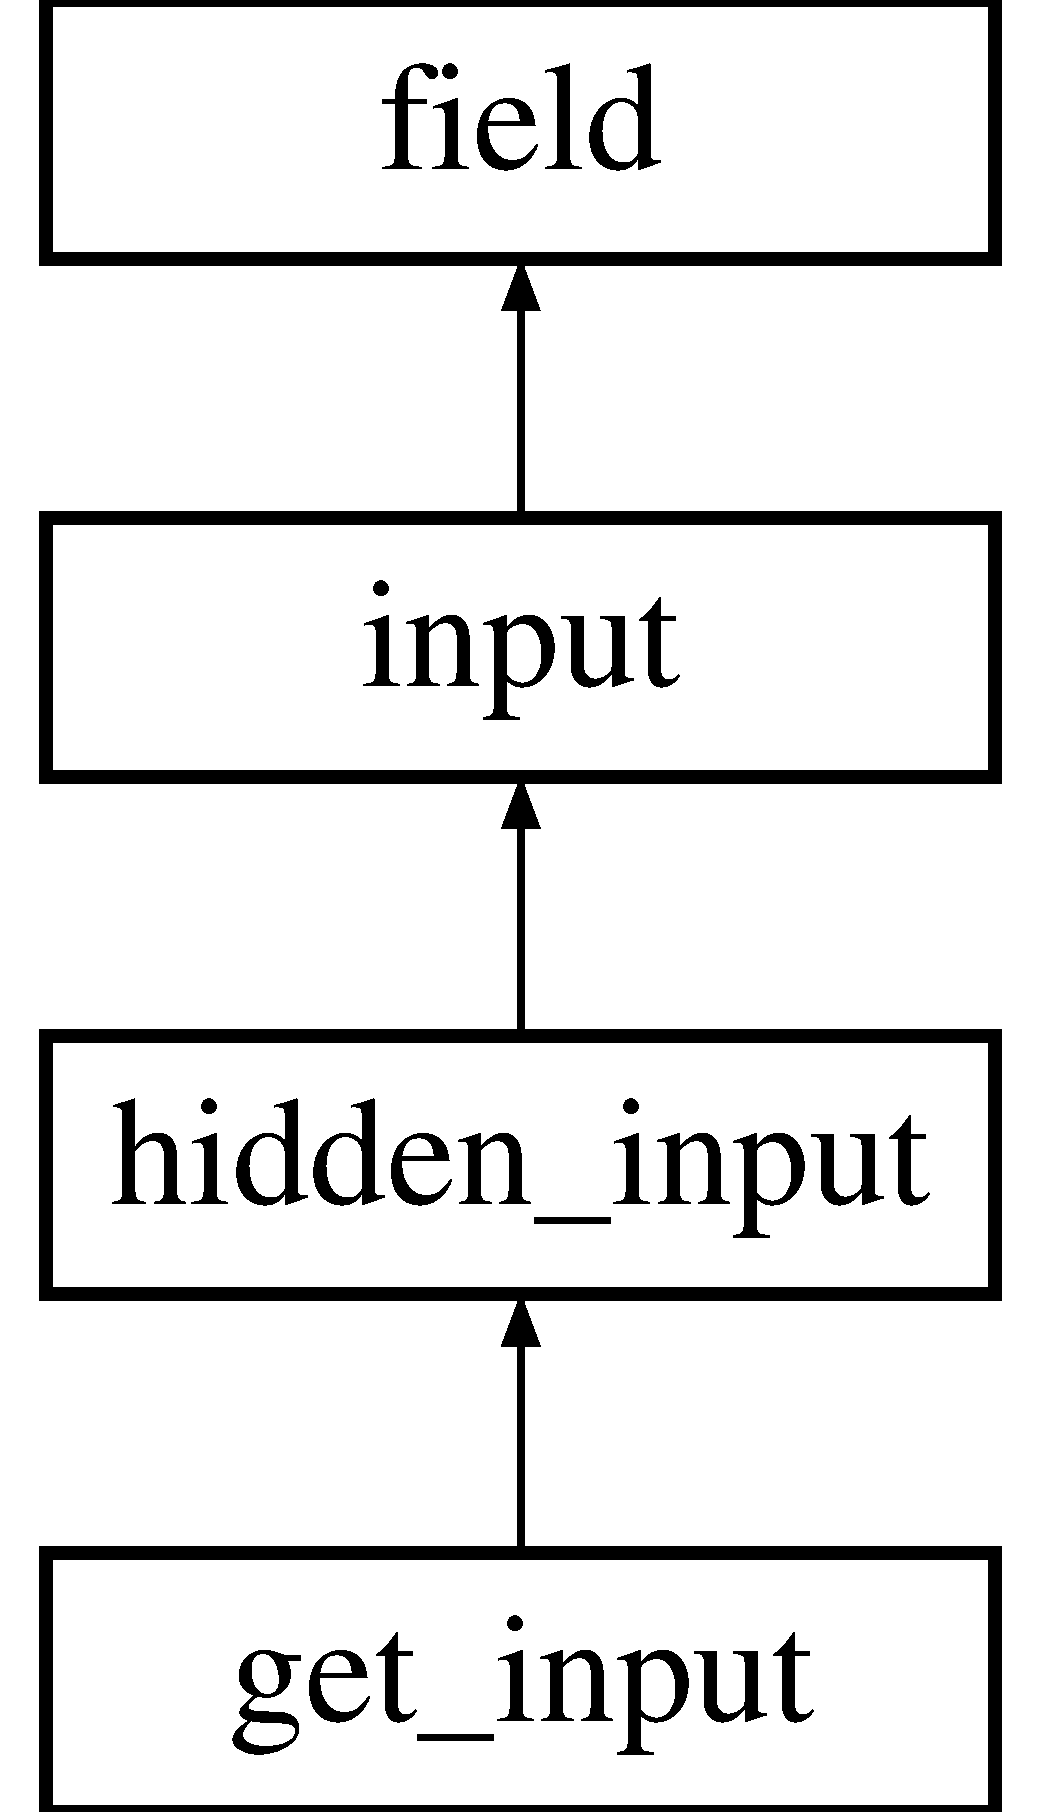
\includegraphics[height=3.000000cm]{classhidden__input}
\end{center}
\end{figure}
\subsubsection*{Public Member Functions}
\begin{DoxyCompactItemize}
\item 
\hyperlink{classhidden__input_a2aeaf443be73e4259caf9dd2cfdecddf}{hidden\-\_\-input} (\$name, \$value= '', \$sanity\-\_\-func=null, \$valid\-\_\-func=null)
\begin{DoxyCompactList}\small\item\em Constructor, creates an \hyperlink{classhidden__input}{hidden\-\_\-input} object. \end{DoxyCompactList}\item 
\hyperlink{classhidden__input_ab20546aae2284c4b1475854d0326e2e3}{form} (\$errors=array())
\begin{DoxyCompactList}\small\item\em Generates the html for the \hyperlink{classhidden__input}{hidden\-\_\-input} for inclusion in a form. \end{DoxyCompactList}\item 
\hyperlink{classhidden__input_a069e47104ea4bd965718c114013fa96f}{display} ()
\begin{DoxyCompactList}\small\item\em Display the name value pair. \end{DoxyCompactList}\end{DoxyCompactItemize}
\subsubsection*{Additional Inherited Members}


\subsubsection{Detailed Description}
The class \hyperlink{classhidden__input}{hidden\-\_\-input} describes a form element, it's attributes and how it is validated and sanitized. 

Meant to be used with the class forms or it's dervative classes. 

\subsubsection{Member Function Documentation}
\hypertarget{classhidden__input_a069e47104ea4bd965718c114013fa96f}{\index{hidden\-\_\-input@{hidden\-\_\-input}!display@{display}}
\index{display@{display}!hidden_input@{hidden\-\_\-input}}
\paragraph[{display}]{\setlength{\rightskip}{0pt plus 5cm}hidden\-\_\-input\-::display (
\begin{DoxyParamCaption}
{}
\end{DoxyParamCaption}
)}}\label{classhidden__input_a069e47104ea4bd965718c114013fa96f}


Display the name value pair. 

\begin{DoxyReturn}{Returns}
A string containing the formated name value pair for this \hyperlink{classhidden__input}{hidden\-\_\-input}. 
\end{DoxyReturn}


Implements \hyperlink{interfacefield_a6a8bbd656a0e7cab2604f6df859bb60a}{field}.

\hypertarget{classhidden__input_ab20546aae2284c4b1475854d0326e2e3}{\index{hidden\-\_\-input@{hidden\-\_\-input}!form@{form}}
\index{form@{form}!hidden_input@{hidden\-\_\-input}}
\paragraph[{form}]{\setlength{\rightskip}{0pt plus 5cm}hidden\-\_\-input\-::form (
\begin{DoxyParamCaption}
\item[{}]{\$errors = {\ttfamily array()}}
\end{DoxyParamCaption}
)}}\label{classhidden__input_ab20546aae2284c4b1475854d0326e2e3}


Generates the html for the \hyperlink{classhidden__input}{hidden\-\_\-input} for inclusion in a form. 


\begin{DoxyParams}[1]{Parameters}
array & {\em \$errors} & an accoiated array errors. If the field name appears in errors, the field's label will be a class of error. \\
\hline
\end{DoxyParams}
\begin{DoxyReturn}{Returns}
array with two elements 'html' the H\-T\-M\-L of the \hyperlink{classhidden__input}{hidden\-\_\-input} field and 'js' any Java\-Script that would assoicated with it (empty for basic \hyperlink{classhidden__input}{hidden\-\_\-input} types at this time). 
\end{DoxyReturn}


Implements \hyperlink{interfacefield_a1b51c4b8b01f77a26eda359e1fc0fb4c}{field}.

\hypertarget{classhidden__input_a2aeaf443be73e4259caf9dd2cfdecddf}{\index{hidden\-\_\-input@{hidden\-\_\-input}!hidden\-\_\-input@{hidden\-\_\-input}}
\index{hidden\-\_\-input@{hidden\-\_\-input}!hidden_input@{hidden\-\_\-input}}
\paragraph[{hidden\-\_\-input}]{\setlength{\rightskip}{0pt plus 5cm}hidden\-\_\-input\-::hidden\-\_\-input (
\begin{DoxyParamCaption}
\item[{}]{\$name, }
\item[{}]{\$value = {\ttfamily ''}, }
\item[{}]{\$sanity\-\_\-func = {\ttfamily null}, }
\item[{}]{\$valid\-\_\-func = {\ttfamily null}}
\end{DoxyParamCaption}
)}}\label{classhidden__input_a2aeaf443be73e4259caf9dd2cfdecddf}


Constructor, creates an \hyperlink{classhidden__input}{hidden\-\_\-input} object. 


\begin{DoxyParams}[1]{Parameters}
string & {\em \$name} & The name of the field used to identify this field in the database, and in the form. \\
\hline
mixed & {\em \$value} & The current value of the field. \\
\hline
mixed & {\em \$sanity\-\_\-func} & A function run on this element to sanitize it, if null will use default sanitation and validation using attributes above. \\
\hline
mixed & {\em \$valid\-\_\-func} & A function run on this element to validate it, if null will use default sanitation and validation using attributes above. \\
\hline
\end{DoxyParams}


The documentation for this class was generated from the following file\-:\begin{DoxyCompactItemize}
\item 
\hyperlink{hidden__input_8inc_8php}{hidden\-\_\-input.\-inc.\-php}\end{DoxyCompactItemize}

\hypertarget{classinput}{\subsection{input Class Reference}
\label{classinput}\index{input@{input}}
}


The class input describes a form element, it's attributes and how it is validated and sanitized.  


Inheritance diagram for input\-:\begin{figure}[H]
\begin{center}
\leavevmode
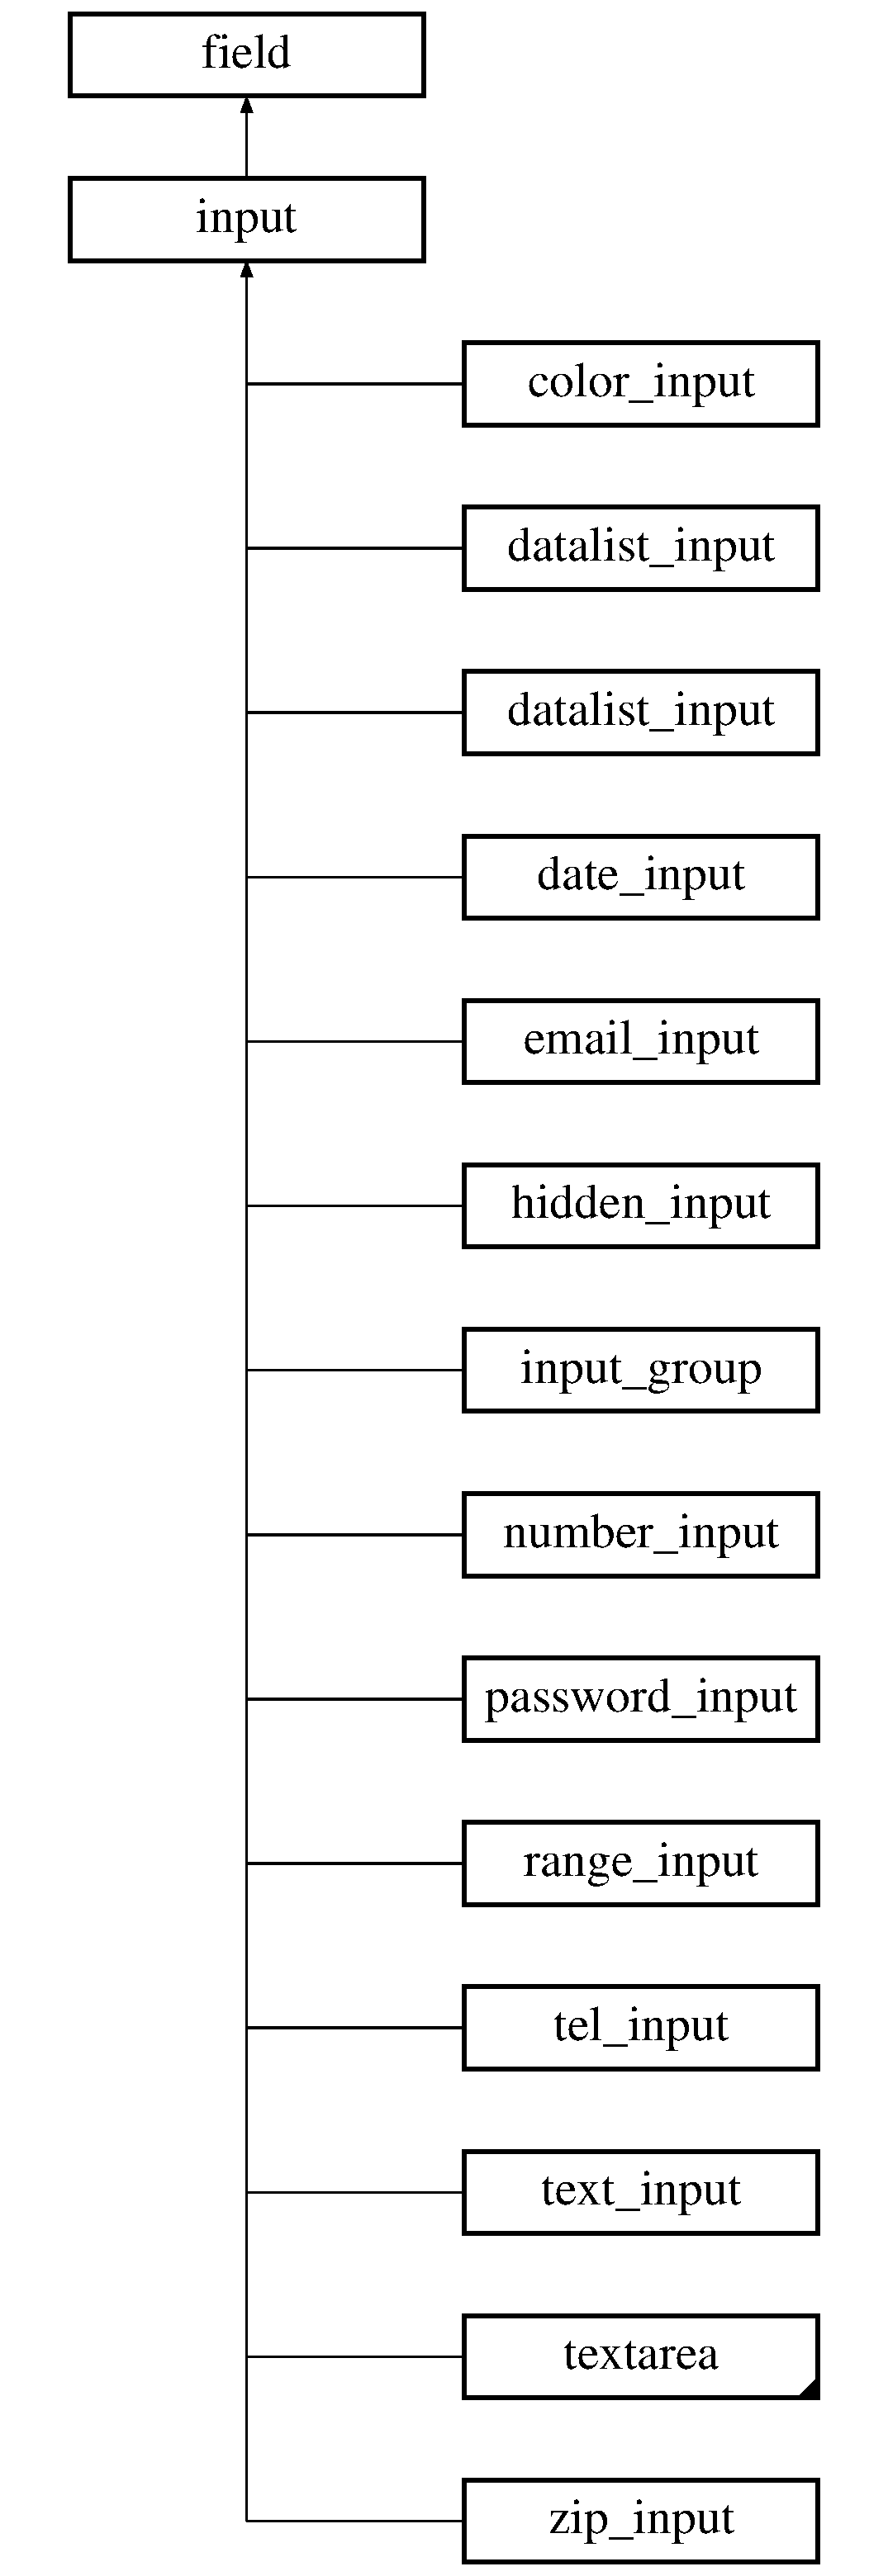
\includegraphics[height=12.000000cm]{classinput}
\end{center}
\end{figure}
\subsubsection*{Public Member Functions}
\begin{DoxyCompactItemize}
\item 
\hyperlink{classinput_a13d088ddc4014c18efd350940632ecc0}{input} (\$label\-\_\-text, \$name, \$type= 'text', \$value= '', \$required=false, \$maxlength= '', \$min= '', \$max= '', \$pattern= '', \$placeholder= '', \$sanity\-\_\-func=null, \$valid\-\_\-func=null)
\begin{DoxyCompactList}\small\item\em Constructor, creates an input object. \end{DoxyCompactList}\item 
\hyperlink{classinput_a83b663057f1d0f61768bc12c5a55f25c}{form} (\$errors=array())
\begin{DoxyCompactList}\small\item\em Generates the html for the input for inclusion in a form. \end{DoxyCompactList}\item 
\hyperlink{classinput_a993053ef011cade1db0ceaccb1f4da53}{display} ()
\begin{DoxyCompactList}\small\item\em Display the name value pair. \end{DoxyCompactList}\item 
\hyperlink{classinput_ab8456d2b5a929801af6fe0b36afd458c}{sanitize} ()
\begin{DoxyCompactList}\small\item\em Sanitizes value to help protect against H\-T\-M\-L, S\-Q\-L, P\-H\-P or other injections. \end{DoxyCompactList}\item 
\hyperlink{classinput_aaf4ed91e7abbc20e2396a4b07dbd031a}{validate} (\$errors=array())
\begin{DoxyCompactList}\small\item\em Validates input's value, and adds errors to the \$errors array if the value isn't valid, based on the attributes of this object or the input's valid\-\_\-func. \end{DoxyCompactList}\item 
\hypertarget{classinput_a1b3bcdbb596a1154a944a169ac67f547}{\hyperlink{classinput_a1b3bcdbb596a1154a944a169ac67f547}{get\-\_\-value} ()}\label{classinput_a1b3bcdbb596a1154a944a169ac67f547}

\begin{DoxyCompactList}\small\item\em Inspector function for this input's value \$return The current value of this input. \end{DoxyCompactList}\item 
\hyperlink{classinput_a2383e00d55bf3dbcc7071b2fe1336aec}{set\-\_\-value} (\$v)
\begin{DoxyCompactList}\small\item\em Mutator function for this input's value. \end{DoxyCompactList}\item 
\hyperlink{classinput_a78f0cd122c69a6f62875152c0cfc9bc2}{values} (\$values)
\begin{DoxyCompactList}\small\item\em Takes an assoicated array of values and assigns the values to input fileds, and the id of this form. \end{DoxyCompactList}\end{DoxyCompactItemize}
\subsubsection*{Public Attributes}
\begin{DoxyCompactItemize}
\item 
\hypertarget{classinput_aed2f7eacbada521eb92809232ad75ca3}{{\bfseries \$label\-\_\-text}}\label{classinput_aed2f7eacbada521eb92809232ad75ca3}

\item 
\hypertarget{classinput_a0cbae4dc5f240d27d6e6d4096e88ad97}{{\bfseries \$name}}\label{classinput_a0cbae4dc5f240d27d6e6d4096e88ad97}

\item 
\hypertarget{classinput_a63d0edb1fac60fb8c53f35a860a8b645}{{\bfseries \$type}}\label{classinput_a63d0edb1fac60fb8c53f35a860a8b645}

\item 
\hypertarget{classinput_a1dc6911d9c8cb9fbac36a50cf57ef589}{{\bfseries \$value}}\label{classinput_a1dc6911d9c8cb9fbac36a50cf57ef589}

\item 
\hypertarget{classinput_a864eeca6da6bd93b04ace1dedb70d0b7}{{\bfseries \$min}}\label{classinput_a864eeca6da6bd93b04ace1dedb70d0b7}

\item 
\hypertarget{classinput_a332378c7b51bb60333d74473b15a5a8b}{{\bfseries \$max}}\label{classinput_a332378c7b51bb60333d74473b15a5a8b}

\item 
\hypertarget{classinput_ae5486c2624c42649b39355332ced3b06}{{\bfseries \$maxlength}}\label{classinput_ae5486c2624c42649b39355332ced3b06}

\item 
\hypertarget{classinput_ac053166030c96a0f0f450e2af7f9eb3b}{{\bfseries \$pattern}}\label{classinput_ac053166030c96a0f0f450e2af7f9eb3b}

\item 
\hypertarget{classinput_a2cb1d88c81d62d30346f888f74772891}{{\bfseries \$required}}\label{classinput_a2cb1d88c81d62d30346f888f74772891}

\item 
\hypertarget{classinput_a0e5ba6b06baea9c597e5656c3adaee0f}{{\bfseries \$placeholder}}\label{classinput_a0e5ba6b06baea9c597e5656c3adaee0f}

\item 
\hypertarget{classinput_ae124da9ea57f47a12780632c6f9bd615}{{\bfseries \$sanity\-\_\-func}}\label{classinput_ae124da9ea57f47a12780632c6f9bd615}

\item 
\hypertarget{classinput_a12410e036b17064b74b940980be5d4aa}{{\bfseries \$valid\-\_\-func}}\label{classinput_a12410e036b17064b74b940980be5d4aa}

\end{DoxyCompactItemize}


\subsubsection{Detailed Description}
The class input describes a form element, it's attributes and how it is validated and sanitized. 

Meant to be used with the class forms or it's dervative classes. 

\subsubsection{Member Function Documentation}
\hypertarget{classinput_a993053ef011cade1db0ceaccb1f4da53}{\index{input@{input}!display@{display}}
\index{display@{display}!input@{input}}
\paragraph[{display}]{\setlength{\rightskip}{0pt plus 5cm}input\-::display (
\begin{DoxyParamCaption}
{}
\end{DoxyParamCaption}
)}}\label{classinput_a993053ef011cade1db0ceaccb1f4da53}


Display the name value pair. 

\begin{DoxyReturn}{Returns}
A string containing the formated name value pair for this input. 
\end{DoxyReturn}


Implements \hyperlink{interfacefield_a6a8bbd656a0e7cab2604f6df859bb60a}{field}.

\hypertarget{classinput_a83b663057f1d0f61768bc12c5a55f25c}{\index{input@{input}!form@{form}}
\index{form@{form}!input@{input}}
\paragraph[{form}]{\setlength{\rightskip}{0pt plus 5cm}input\-::form (
\begin{DoxyParamCaption}
\item[{}]{\$errors = {\ttfamily array()}}
\end{DoxyParamCaption}
)}}\label{classinput_a83b663057f1d0f61768bc12c5a55f25c}


Generates the html for the input for inclusion in a form. 


\begin{DoxyParams}[1]{Parameters}
array & {\em \$errors} & an accoiated array errors. If the field name appears in errors, the field's label will be a class of error. \\
\hline
\end{DoxyParams}
\begin{DoxyReturn}{Returns}
array with two elements 'html' the H\-T\-M\-L of the input field and 'js' any Java\-Script that would assoicated with it (empty for basic input types at this time). 
\end{DoxyReturn}


Implements \hyperlink{interfacefield_a1b51c4b8b01f77a26eda359e1fc0fb4c}{field}.

\hypertarget{classinput_a13d088ddc4014c18efd350940632ecc0}{\index{input@{input}!input@{input}}
\index{input@{input}!input@{input}}
\paragraph[{input}]{\setlength{\rightskip}{0pt plus 5cm}input\-::input (
\begin{DoxyParamCaption}
\item[{}]{\$label\-\_\-text, }
\item[{}]{\$name, }
\item[{}]{\$type = {\ttfamily 'text'}, }
\item[{}]{\$value = {\ttfamily ''}, }
\item[{}]{\$required = {\ttfamily false}, }
\item[{}]{\$maxlength = {\ttfamily ''}, }
\item[{}]{\$min = {\ttfamily ''}, }
\item[{}]{\$max = {\ttfamily ''}, }
\item[{}]{\$pattern = {\ttfamily ''}, }
\item[{}]{\$placeholder = {\ttfamily ''}, }
\item[{}]{\$sanity\-\_\-func = {\ttfamily null}, }
\item[{}]{\$valid\-\_\-func = {\ttfamily null}}
\end{DoxyParamCaption}
)}}\label{classinput_a13d088ddc4014c18efd350940632ecc0}


Constructor, creates an input object. 


\begin{DoxyParams}[1]{Parameters}
string & {\em \$label\-\_\-text} & The text label on the form field. \\
\hline
string & {\em \$name} & The name of the field used to identify this field in the database, and in the form. \\
\hline
string & {\em \$type} & The type of input, should be a valid H\-T\-M\-L type. \\
\hline
mixed & {\em \$value} & The current value of the field. \\
\hline
bool & {\em \$required} & Boolean value, weather or not the user is required to enter a value for the field. \\
\hline
mixed & {\em \$maxlength} & The maximum characters this field's value can have, and still be valid. null or empty string will make this be ignored. \\
\hline
mixes & {\em \$min} & The minimum value allowed for this imput, when type is date, time or some type that has a numberic value. null or empty string willl make this be ignored. \\
\hline
string & {\em \$pattern} & The regex pattern that this field's value must match to be valid. null or empty string will make this ignored. \\
\hline
string & {\em \$placeholder} & The placeholder text for this item. null or empty string will suppress this attribute from being printed. \\
\hline
mixed & {\em \$sanity\-\_\-func} & A function run on this element to sanitize it, if null will use default sanitation and validation using attributes above. \\
\hline
mixed & {\em \$valid\-\_\-func} & A function run on this element to validate it, if null will use default sanitation and validation using attributes above. \\
\hline
\end{DoxyParams}
\hypertarget{classinput_ab8456d2b5a929801af6fe0b36afd458c}{\index{input@{input}!sanitize@{sanitize}}
\index{sanitize@{sanitize}!input@{input}}
\paragraph[{sanitize}]{\setlength{\rightskip}{0pt plus 5cm}input\-::sanitize (
\begin{DoxyParamCaption}
{}
\end{DoxyParamCaption}
)}}\label{classinput_ab8456d2b5a929801af6fe0b36afd458c}


Sanitizes value to help protect against H\-T\-M\-L, S\-Q\-L, P\-H\-P or other injections. 

Returns false if the value can't be cleaned in a sensible way. \begin{DoxyReturn}{Returns}
mixed often the value of the field or true if sanitization occured properly, but false if we are unable to sanitize. Use identical test '===' instaead of equality as input may have values of '' or 0. 
\end{DoxyReturn}


Implements \hyperlink{interfacefield_a3ed132df10731b5ebe33acc44ac03c85}{field}.

\hypertarget{classinput_a2383e00d55bf3dbcc7071b2fe1336aec}{\index{input@{input}!set\-\_\-value@{set\-\_\-value}}
\index{set\-\_\-value@{set\-\_\-value}!input@{input}}
\paragraph[{set\-\_\-value}]{\setlength{\rightskip}{0pt plus 5cm}input\-::set\-\_\-value (
\begin{DoxyParamCaption}
\item[{}]{\$v}
\end{DoxyParamCaption}
)}}\label{classinput_a2383e00d55bf3dbcc7071b2fe1336aec}


Mutator function for this input's value. 


\begin{DoxyParams}[1]{Parameters}
mixed & {\em \$v} & The new value of this input \#post The value of this input will be set to \$v \\
\hline
\end{DoxyParams}
\hypertarget{classinput_aaf4ed91e7abbc20e2396a4b07dbd031a}{\index{input@{input}!validate@{validate}}
\index{validate@{validate}!input@{input}}
\paragraph[{validate}]{\setlength{\rightskip}{0pt plus 5cm}input\-::validate (
\begin{DoxyParamCaption}
\item[{}]{\$errors = {\ttfamily array()}}
\end{DoxyParamCaption}
)}}\label{classinput_aaf4ed91e7abbc20e2396a4b07dbd031a}


Validates input's value, and adds errors to the \$errors array if the value isn't valid, based on the attributes of this object or the input's valid\-\_\-func. 


\begin{DoxyParams}[1]{Parameters}
array & {\em \$errors} & an array of errors previously in the form, errors will be added to the array and the array returned. \\
\hline
\end{DoxyParams}
\begin{DoxyReturn}{Returns}
array errors is returned, possibly with errors appended. 
\end{DoxyReturn}


Implements \hyperlink{interfacefield_a352b92f9e8dce69191bad79bdc5d972b}{field}.

\hypertarget{classinput_a78f0cd122c69a6f62875152c0cfc9bc2}{\index{input@{input}!values@{values}}
\index{values@{values}!input@{input}}
\paragraph[{values}]{\setlength{\rightskip}{0pt plus 5cm}input\-::values (
\begin{DoxyParamCaption}
\item[{}]{\$values}
\end{DoxyParamCaption}
)}}\label{classinput_a78f0cd122c69a6f62875152c0cfc9bc2}


Takes an assoicated array of values and assigns the values to input fileds, and the id of this form. 


\begin{DoxyParams}[1]{Parameters}
array & {\em \$values} & an associated array of values. Ignores values of keys that aren't fields in this form. \\
\hline
\end{DoxyParams}


Implements \hyperlink{interfacefield_a54958a09bc0dcd947d611b14741c5996}{field}.



The documentation for this class was generated from the following file\-:\begin{DoxyCompactItemize}
\item 
\hyperlink{input_8inc_8php}{input.\-inc.\-php}\end{DoxyCompactItemize}

\hypertarget{classinput__group}{\subsection{input\-\_\-group Class Reference}
\label{classinput__group}\index{input\-\_\-group@{input\-\_\-group}}
}


Defines a group of related inputs like raido buttons or checkboxes that have the same name, but different values.  


Inheritance diagram for input\-\_\-group\-:\begin{figure}[H]
\begin{center}
\leavevmode
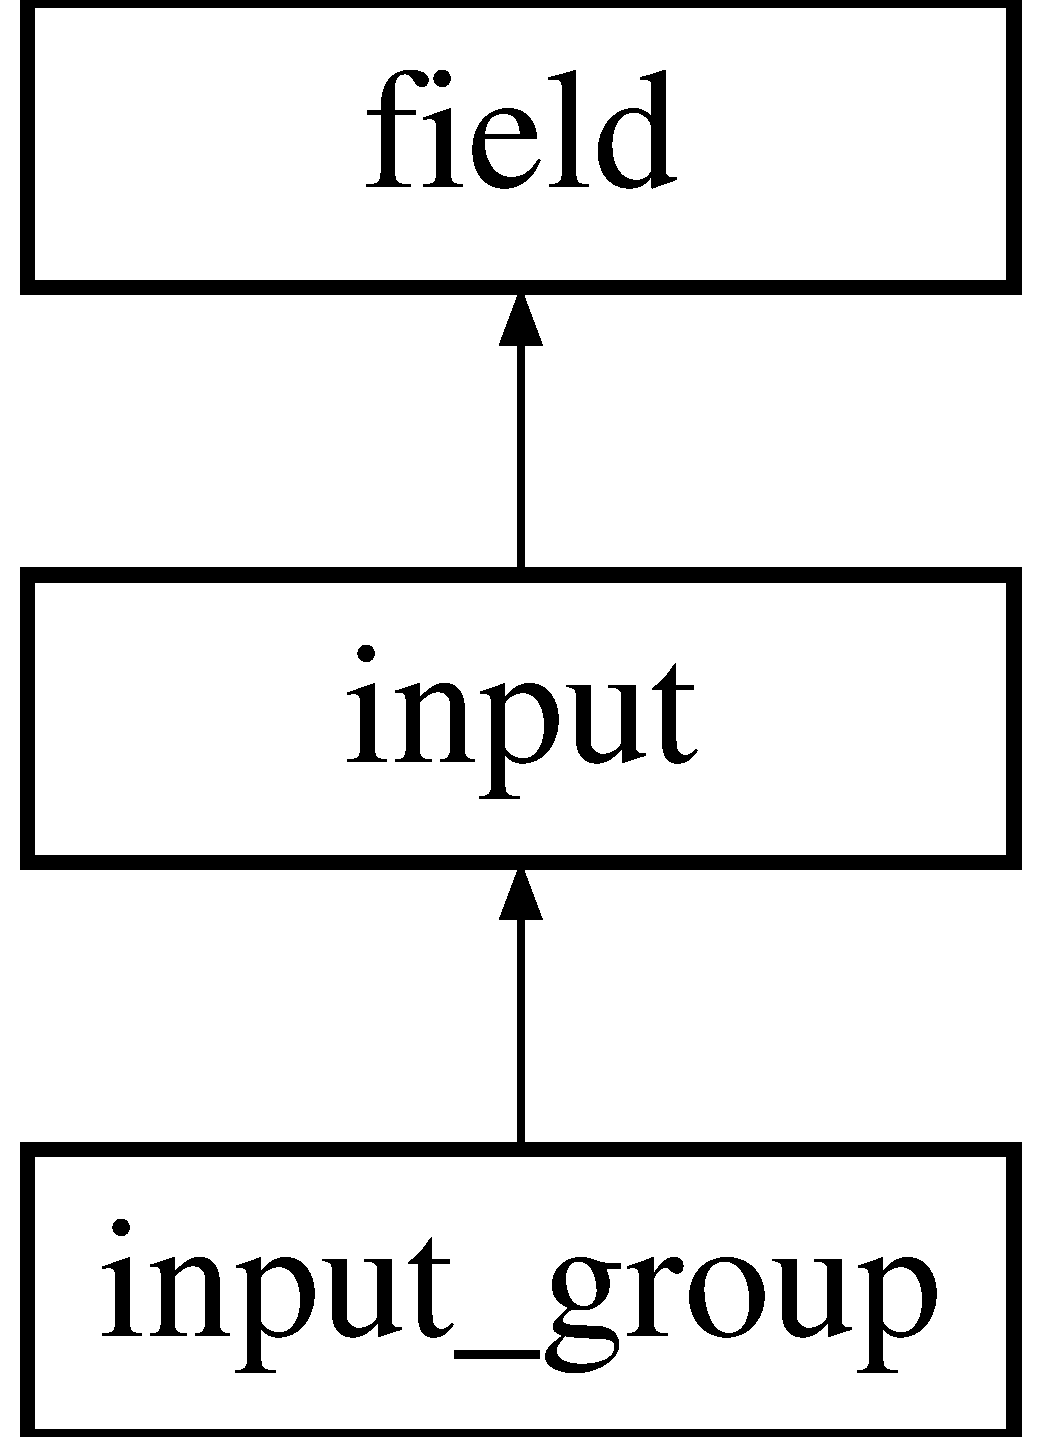
\includegraphics[height=3.000000cm]{classinput__group}
\end{center}
\end{figure}
\subsubsection*{Public Member Functions}
\begin{DoxyCompactItemize}
\item 
\hyperlink{classinput__group_aef532e921771fbfccacbdefba1db7dce}{input\-\_\-group} (\$label\-\_\-text, \$name, \$value\-\_\-list, \$type= 'checkbox', \$value= '', \$required= '', \$placeholder= '', \$sanity\-\_\-func=null, \$valid\-\_\-func=null)
\begin{DoxyCompactList}\small\item\em Constructor for \hyperlink{classinput__group}{input\-\_\-group} object. \end{DoxyCompactList}\item 
\hyperlink{classinput__group_a67f5d8e4ac86e75313e8d0d8696b7b35}{form} (\$errors=array())
\begin{DoxyCompactList}\small\item\em Generates the H\-T\-M\-L for this input to be included in a form. \end{DoxyCompactList}\item 
\hyperlink{classinput__group_a91e1b3cab54b81c21ab5f88a2f4f5c6a}{display} ()
\begin{DoxyCompactList}\small\item\em Display the name value pair. \end{DoxyCompactList}\item 
\hyperlink{classinput__group_aac74288da2e6c962dc507ccaa1f8f450}{display\-\_\-text} ()
\begin{DoxyCompactList}\small\item\em Display the name value pair. \end{DoxyCompactList}\item 
\hyperlink{classinput__group_a4f0f7f8aeb74550c99114f28dca449cb}{sanitize} ()
\begin{DoxyCompactList}\small\item\em Sanitize this form's values. \end{DoxyCompactList}\item 
\hyperlink{classinput__group_ae0461a6034effccc3ca6bf34b6539cdd}{validate} (\$errors=array())
\begin{DoxyCompactList}\small\item\em Validate this form's values. \end{DoxyCompactList}\end{DoxyCompactItemize}
\subsubsection*{Public Attributes}
\begin{DoxyCompactItemize}
\item 
\hypertarget{classinput__group_ae3e73495f83432370ed5acb0f81e1ba1}{{\bfseries \$value\-\_\-list}}\label{classinput__group_ae3e73495f83432370ed5acb0f81e1ba1}

\end{DoxyCompactItemize}


\subsubsection{Detailed Description}
Defines a group of related inputs like raido buttons or checkboxes that have the same name, but different values. 

\subsubsection{Member Function Documentation}
\hypertarget{classinput__group_a91e1b3cab54b81c21ab5f88a2f4f5c6a}{\index{input\-\_\-group@{input\-\_\-group}!display@{display}}
\index{display@{display}!input_group@{input\-\_\-group}}
\paragraph[{display}]{\setlength{\rightskip}{0pt plus 5cm}input\-\_\-group\-::display (
\begin{DoxyParamCaption}
{}
\end{DoxyParamCaption}
)}}\label{classinput__group_a91e1b3cab54b81c21ab5f88a2f4f5c6a}


Display the name value pair. 

\begin{DoxyReturn}{Returns}
A string containing the H\-T\-M\-L formated name value pair for this input. 
\end{DoxyReturn}


Implements \hyperlink{interfacefield_a6a8bbd656a0e7cab2604f6df859bb60a}{field}.

\hypertarget{classinput__group_aac74288da2e6c962dc507ccaa1f8f450}{\index{input\-\_\-group@{input\-\_\-group}!display\-\_\-text@{display\-\_\-text}}
\index{display\-\_\-text@{display\-\_\-text}!input_group@{input\-\_\-group}}
\paragraph[{display\-\_\-text}]{\setlength{\rightskip}{0pt plus 5cm}input\-\_\-group\-::display\-\_\-text (
\begin{DoxyParamCaption}
{}
\end{DoxyParamCaption}
)}}\label{classinput__group_aac74288da2e6c962dc507ccaa1f8f450}


Display the name value pair. 

\begin{DoxyReturn}{Returns}
A string containing the text formated name value pair for this input. 
\end{DoxyReturn}


Implements \hyperlink{interfacefield_a5e8d3e49ab5fba3956b7a297535806dc}{field}.

\hypertarget{classinput__group_a67f5d8e4ac86e75313e8d0d8696b7b35}{\index{input\-\_\-group@{input\-\_\-group}!form@{form}}
\index{form@{form}!input_group@{input\-\_\-group}}
\paragraph[{form}]{\setlength{\rightskip}{0pt plus 5cm}input\-\_\-group\-::form (
\begin{DoxyParamCaption}
\item[{}]{\$errors = {\ttfamily array()}}
\end{DoxyParamCaption}
)}}\label{classinput__group_a67f5d8e4ac86e75313e8d0d8696b7b35}


Generates the H\-T\-M\-L for this input to be included in a form. 


\begin{DoxyParams}[1]{Parameters}
array & {\em \$errors} & an array of accumulated errors. \\
\hline
\end{DoxyParams}
\begin{DoxyReturn}{Returns}
array with two elements 'html'=$>$ The H\-T\-M\-L for the object, 'js' =$>$ Any J\-S for the element (currently none). 
\end{DoxyReturn}


Implements \hyperlink{interfacefield_a1b51c4b8b01f77a26eda359e1fc0fb4c}{field}.

\hypertarget{classinput__group_aef532e921771fbfccacbdefba1db7dce}{\index{input\-\_\-group@{input\-\_\-group}!input\-\_\-group@{input\-\_\-group}}
\index{input\-\_\-group@{input\-\_\-group}!input_group@{input\-\_\-group}}
\paragraph[{input\-\_\-group}]{\setlength{\rightskip}{0pt plus 5cm}input\-\_\-group\-::input\-\_\-group (
\begin{DoxyParamCaption}
\item[{}]{\$label\-\_\-text, }
\item[{}]{\$name, }
\item[{}]{\$value\-\_\-list, }
\item[{}]{\$type = {\ttfamily 'checkbox'}, }
\item[{}]{\$value = {\ttfamily ''}, }
\item[{}]{\$required = {\ttfamily ''}, }
\item[{}]{\$placeholder = {\ttfamily ''}, }
\item[{}]{\$sanity\-\_\-func = {\ttfamily null}, }
\item[{}]{\$valid\-\_\-func = {\ttfamily null}}
\end{DoxyParamCaption}
)}}\label{classinput__group_aef532e921771fbfccacbdefba1db7dce}


Constructor for \hyperlink{classinput__group}{input\-\_\-group} object. 


\begin{DoxyParams}{Parameters}
{\em \$label\-\_\-text} & The label for the group, will be displayed as the legend in the rendered html. \\
\hline
{\em \$name} & The name of the item in html, and the fields of the form. \\
\hline
{\em \$value\-\_\-list} & the values for the input tags. \\
\hline
{\em \$type} & the H\-T\-M\-L type of input each will be. \\
\hline
{\em \$value} & an array or single value, the currently checked/activated inputs. \\
\hline
{\em \$required} & boolean on weather or not a selection is required. \\
\hline
{\em \$placeholder} & The placeholder text for this item. null or empty string will suppress this attribute from being printed. \\
\hline
{\em \$sanity\-\_\-func} & A function run on this element to sanitize it, if null will use default sanitation and validation using attributes above. \\
\hline
{\em \$valid\-\_\-func} & A function run on this element to validate it, if null will use default sanitation and validation using attributes above. \\
\hline
\end{DoxyParams}
\begin{DoxyRefDesc}{Todo}
\item[\hyperlink{todo__todo000011}{Todo}]work out required, and single values. \end{DoxyRefDesc}
\hypertarget{classinput__group_a4f0f7f8aeb74550c99114f28dca449cb}{\index{input\-\_\-group@{input\-\_\-group}!sanitize@{sanitize}}
\index{sanitize@{sanitize}!input_group@{input\-\_\-group}}
\paragraph[{sanitize}]{\setlength{\rightskip}{0pt plus 5cm}input\-\_\-group\-::sanitize (
\begin{DoxyParamCaption}
{}
\end{DoxyParamCaption}
)}}\label{classinput__group_a4f0f7f8aeb74550c99114f28dca449cb}


Sanitize this form's values. 

\begin{DoxyRefDesc}{Todo}
\item[\hyperlink{todo__todo000012}{Todo}]Write this. \end{DoxyRefDesc}
\begin{DoxyRefDesc}{Bug}
\item[\hyperlink{bug__bug000001}{Bug}]always returns true. \end{DoxyRefDesc}


Implements \hyperlink{interfacefield_a3ed132df10731b5ebe33acc44ac03c85}{field}.

\hypertarget{classinput__group_ae0461a6034effccc3ca6bf34b6539cdd}{\index{input\-\_\-group@{input\-\_\-group}!validate@{validate}}
\index{validate@{validate}!input_group@{input\-\_\-group}}
\paragraph[{validate}]{\setlength{\rightskip}{0pt plus 5cm}input\-\_\-group\-::validate (
\begin{DoxyParamCaption}
\item[{}]{\$errors = {\ttfamily array()}}
\end{DoxyParamCaption}
)}}\label{classinput__group_ae0461a6034effccc3ca6bf34b6539cdd}


Validate this form's values. 

\begin{DoxyRefDesc}{Todo}
\item[\hyperlink{todo__todo000013}{Todo}]Write this. \end{DoxyRefDesc}
\begin{DoxyRefDesc}{Bug}
\item[\hyperlink{bug__bug000002}{Bug}]always returns true. \end{DoxyRefDesc}


Implements \hyperlink{interfacefield_a352b92f9e8dce69191bad79bdc5d972b}{field}.



The documentation for this class was generated from the following file\-:\begin{DoxyCompactItemize}
\item 
\hyperlink{input__group_8inc_8php}{input\-\_\-group.\-inc.\-php}\end{DoxyCompactItemize}

\hypertarget{classmessage}{\subsection{message Class Reference}
\label{classmessage}\index{message@{message}}
}
\subsubsection*{Public Member Functions}
\begin{DoxyCompactItemize}
\item 
\hypertarget{classmessage_a9c834e519b14b1a80bbae503c87c86eb}{{\bfseries message} (\$msg, \$condition=null)}\label{classmessage_a9c834e519b14b1a80bbae503c87c86eb}

\item 
\hypertarget{classmessage_af4d6453d37e1b4efb7c037b85f1817b1}{{\bfseries notify} (\$\hyperlink{classevent}{event})}\label{classmessage_af4d6453d37e1b4efb7c037b85f1817b1}

\item 
\hypertarget{classmessage_afcfe62089a61d723fa85a2c7cb2c46e6}{{\bfseries values} (\$v)}\label{classmessage_afcfe62089a61d723fa85a2c7cb2c46e6}

\item 
\hypertarget{classmessage_aa0fe8c20e66d9c62ae74c2b8139ffdc9}{{\bfseries form} (\$the\-\_\-form)}\label{classmessage_aa0fe8c20e66d9c62ae74c2b8139ffdc9}

\end{DoxyCompactItemize}
\subsubsection*{Public Attributes}
\begin{DoxyCompactItemize}
\item 
\hypertarget{classmessage_a44c174aa0f49e4b798fc1f537c2b73c5}{{\bfseries \$msg}}\label{classmessage_a44c174aa0f49e4b798fc1f537c2b73c5}

\item 
\hypertarget{classmessage_a9055b182ecf30cacc77a75676501f1fc}{{\bfseries \$condition}}\label{classmessage_a9055b182ecf30cacc77a75676501f1fc}

\end{DoxyCompactItemize}


The documentation for this class was generated from the following file\-:\begin{DoxyCompactItemize}
\item 
actions.\-inc.\-php\end{DoxyCompactItemize}

\hypertarget{classnumber__input}{\subsection{number\-\_\-input Class Reference}
\label{classnumber__input}\index{number\-\_\-input@{number\-\_\-input}}
}


This convience class allows easy creation of an input with type=\char`\"{}number\char`\"{}.  


Inheritance diagram for number\-\_\-input\-:\begin{figure}[H]
\begin{center}
\leavevmode
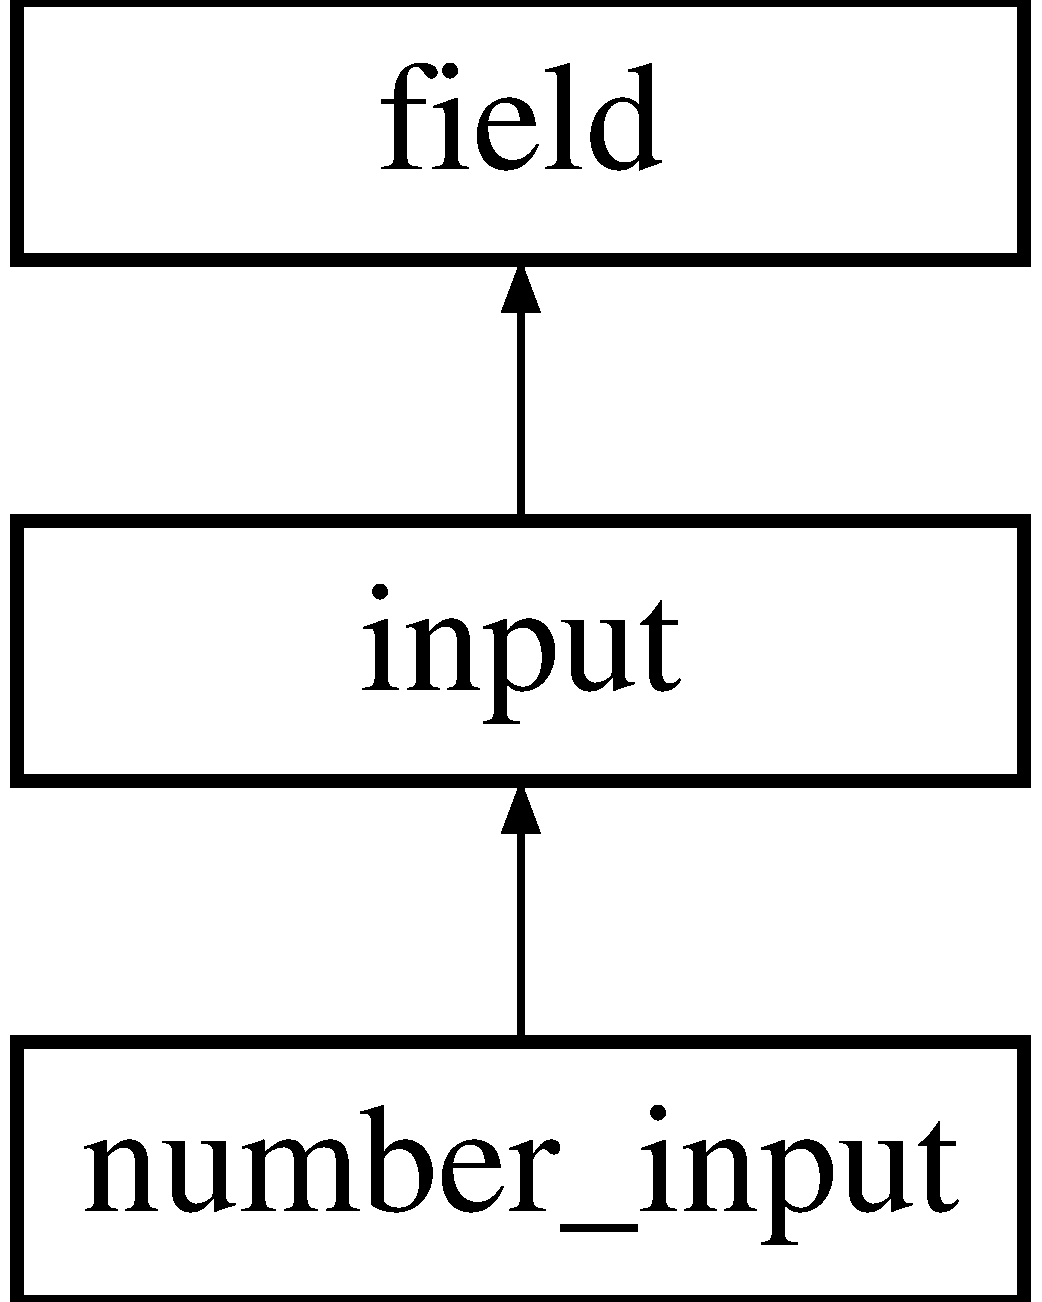
\includegraphics[height=3.000000cm]{classnumber__input}
\end{center}
\end{figure}
\subsubsection*{Public Member Functions}
\begin{DoxyCompactItemize}
\item 
\hyperlink{classnumber__input_a6850b71ee7cf3f7733bf84fe7dd085bb}{\-\_\-\-\_\-construct} (\$label\-\_\-text, \$name, \$value, \$required=false, \$min= '', \$max= '', \$placeholder= '', \$sanity\-\_\-func=null, \$valid\-\_\-func=null)
\begin{DoxyCompactList}\small\item\em Constructor for \hyperlink{classnumber__input}{number\-\_\-input}. \end{DoxyCompactList}\item 
\hyperlink{classnumber__input_ac3cbe1ec02ef79588e1dbf5d2360b84e}{get\-\_\-value} ()
\begin{DoxyCompactList}\small\item\em Inspector for the value of this input. \end{DoxyCompactList}\item 
\hyperlink{classnumber__input_a8026b12c0bf4c8ea0ad303a532ed7230}{set\-\_\-value} (\$v)
\begin{DoxyCompactList}\small\item\em Mutator for the value of this input. \end{DoxyCompactList}\end{DoxyCompactItemize}
\subsubsection*{Additional Inherited Members}


\subsubsection{Detailed Description}
This convience class allows easy creation of an input with type=\char`\"{}number\char`\"{}. 



\subsubsection{Constructor \& Destructor Documentation}
\hypertarget{classnumber__input_a6850b71ee7cf3f7733bf84fe7dd085bb}{\index{number\-\_\-input@{number\-\_\-input}!\-\_\-\-\_\-construct@{\-\_\-\-\_\-construct}}
\index{\-\_\-\-\_\-construct@{\-\_\-\-\_\-construct}!number_input@{number\-\_\-input}}
\paragraph[{\-\_\-\-\_\-construct}]{\setlength{\rightskip}{0pt plus 5cm}number\-\_\-input\-::\-\_\-\-\_\-construct (
\begin{DoxyParamCaption}
\item[{}]{\$label\-\_\-text, }
\item[{}]{\$name, }
\item[{}]{\$value, }
\item[{}]{\$required = {\ttfamily false}, }
\item[{}]{\$min = {\ttfamily ''}, }
\item[{}]{\$max = {\ttfamily ''}, }
\item[{}]{\$placeholder = {\ttfamily ''}, }
\item[{}]{\$sanity\-\_\-func = {\ttfamily null}, }
\item[{}]{\$valid\-\_\-func = {\ttfamily null}}
\end{DoxyParamCaption}
)}}\label{classnumber__input_a6850b71ee7cf3f7733bf84fe7dd085bb}


Constructor for \hyperlink{classnumber__input}{number\-\_\-input}. 


\begin{DoxyParams}{Parameters}
{\em \$label\-\_\-text} & The text label for this \hyperlink{classnumber__input}{number\-\_\-input}. \\
\hline
{\em \$name} & The name of this field for internal use. (i.\-e. the name attribute in the render H\-T\-M\-L and/or used in form) \\
\hline
{\em \$value} & The current value of this input. Optional. Default is ''. \\
\hline
{\em \$required} & Weather or not the user is required to enter this field. This effects both H\-T\-M\-L5 element and validation. Optional. Default is false. \\
\hline
{\em \$min} & The minium value this \hyperlink{classnumber__input}{number\-\_\-input} allows, used in validation and H\-T\-M\-L5 min attribute. Optional. If not set, or set to '', this attribute is ignored. \\
\hline
{\em \$max} & The maximum value this \hyperlink{classnumber__input}{number\-\_\-input} allows, used in validation and H\-T\-M\-L5 max attribute. Optional. If not set, or set to '', this attribute is ignored. \\
\hline
{\em \$placeholder} & This is used for the H\-T\-M\-L5 placeholder attribute. Optional. Default is false. \\
\hline
{\em \$sanity\-\_\-func} & Optional function for sanitization. Defualt is null. \\
\hline
{\em \$valid\-\_\-func} & Optional function for validation. Default is null. \\
\hline
\end{DoxyParams}


\subsubsection{Member Function Documentation}
\hypertarget{classnumber__input_ac3cbe1ec02ef79588e1dbf5d2360b84e}{\index{number\-\_\-input@{number\-\_\-input}!get\-\_\-value@{get\-\_\-value}}
\index{get\-\_\-value@{get\-\_\-value}!number_input@{number\-\_\-input}}
\paragraph[{get\-\_\-value}]{\setlength{\rightskip}{0pt plus 5cm}number\-\_\-input\-::get\-\_\-value (
\begin{DoxyParamCaption}
{}
\end{DoxyParamCaption}
)}}\label{classnumber__input_ac3cbe1ec02ef79588e1dbf5d2360b84e}


Inspector for the value of this input. 

\begin{DoxyReturn}{Returns}
mixed The value of this input. 
\end{DoxyReturn}
\hypertarget{classnumber__input_a8026b12c0bf4c8ea0ad303a532ed7230}{\index{number\-\_\-input@{number\-\_\-input}!set\-\_\-value@{set\-\_\-value}}
\index{set\-\_\-value@{set\-\_\-value}!number_input@{number\-\_\-input}}
\paragraph[{set\-\_\-value}]{\setlength{\rightskip}{0pt plus 5cm}number\-\_\-input\-::set\-\_\-value (
\begin{DoxyParamCaption}
\item[{}]{\$v}
\end{DoxyParamCaption}
)}}\label{classnumber__input_a8026b12c0bf4c8ea0ad303a532ed7230}


Mutator for the value of this input. 


\begin{DoxyParams}[1]{Parameters}
mixed & {\em \$v} & The new value of this input \\
\hline
\end{DoxyParams}


The documentation for this class was generated from the following file\-:\begin{DoxyCompactItemize}
\item 
\hyperlink{extended__inputs_8inc_8php}{extended\-\_\-inputs.\-inc.\-php}\end{DoxyCompactItemize}

\hypertarget{interfaceobservable}{\subsection{observable Interface Reference}
\label{interfaceobservable}\index{observable@{observable}}
}


Describes objects that are able to be observed by observer objects.  


Inheritance diagram for observable\-:\begin{figure}[H]
\begin{center}
\leavevmode
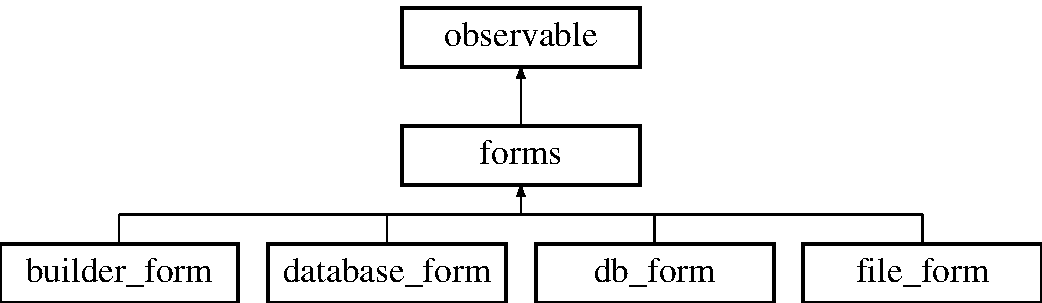
\includegraphics[height=3.000000cm]{interfaceobservable}
\end{center}
\end{figure}
\subsubsection*{Public Member Functions}
\begin{DoxyCompactItemize}
\item 
\hyperlink{interfaceobservable_aa4d6d161d4154a3525e93f6c051e1914}{notify} (\$\hyperlink{classevent}{event})
\begin{DoxyCompactList}\small\item\em Notify observers an \$event has taken place. \end{DoxyCompactList}\item 
\hyperlink{interfaceobservable_aa4c1e85f5ec861411aa1d99ee0471082}{add\-\_\-observer} (\$ob)
\begin{DoxyCompactList}\small\item\em Add an observer to watch \$this object. \end{DoxyCompactList}\item 
\hyperlink{interfaceobservable_aea49f4e7d1c3181031e50c15e0bfd9d4}{remove\-\_\-observer} (\$ob)
\begin{DoxyCompactList}\small\item\em Remove an observer of \$this object. \end{DoxyCompactList}\end{DoxyCompactItemize}


\subsubsection{Detailed Description}
Describes objects that are able to be observed by observer objects. 

\subsubsection{Member Function Documentation}
\hypertarget{interfaceobservable_aa4c1e85f5ec861411aa1d99ee0471082}{\index{observable@{observable}!add\-\_\-observer@{add\-\_\-observer}}
\index{add\-\_\-observer@{add\-\_\-observer}!observable@{observable}}
\paragraph[{add\-\_\-observer}]{\setlength{\rightskip}{0pt plus 5cm}observable\-::add\-\_\-observer (
\begin{DoxyParamCaption}
\item[{}]{\$ob}
\end{DoxyParamCaption}
)}}\label{interfaceobservable_aa4c1e85f5ec861411aa1d99ee0471082}


Add an observer to watch \$this object. 


\begin{DoxyParams}[1]{Parameters}
observer & {\em \$ob} & The object waiting for state change. \\
\hline
\end{DoxyParams}


Implemented in \hyperlink{classforms_a6c88ab2728699cc06ba8110b1f5aacbc}{forms}.

\hypertarget{interfaceobservable_aa4d6d161d4154a3525e93f6c051e1914}{\index{observable@{observable}!notify@{notify}}
\index{notify@{notify}!observable@{observable}}
\paragraph[{notify}]{\setlength{\rightskip}{0pt plus 5cm}observable\-::notify (
\begin{DoxyParamCaption}
\item[{}]{\$event}
\end{DoxyParamCaption}
)}}\label{interfaceobservable_aa4d6d161d4154a3525e93f6c051e1914}


Notify observers an \$event has taken place. 


\begin{DoxyParams}{Parameters}
{\em \$event} & The event that's occured. \\
\hline
\end{DoxyParams}


Implemented in \hyperlink{classforms_a82bc2b5e603ecd535f362c3dfdcae96e}{forms}.

\hypertarget{interfaceobservable_aea49f4e7d1c3181031e50c15e0bfd9d4}{\index{observable@{observable}!remove\-\_\-observer@{remove\-\_\-observer}}
\index{remove\-\_\-observer@{remove\-\_\-observer}!observable@{observable}}
\paragraph[{remove\-\_\-observer}]{\setlength{\rightskip}{0pt plus 5cm}observable\-::remove\-\_\-observer (
\begin{DoxyParamCaption}
\item[{}]{\$ob}
\end{DoxyParamCaption}
)}}\label{interfaceobservable_aea49f4e7d1c3181031e50c15e0bfd9d4}


Remove an observer of \$this object. 


\begin{DoxyParams}[1]{Parameters}
observer & {\em \$ob} & The oberserver we want to remove. \\
\hline
\end{DoxyParams}


Implemented in \hyperlink{classforms_af5c72c905909819f8824958c2faa015d}{forms}.



The documentation for this interface was generated from the following file\-:\begin{DoxyCompactItemize}
\item 
\hyperlink{observable_8inc_8php}{observable.\-inc.\-php}\end{DoxyCompactItemize}

\hypertarget{classobserver}{\subsection{observer Class Reference}
\label{classobserver}\index{observer@{observer}}
}


Impliments the observer in the observer patters.  


\subsubsection*{Public Member Functions}
\begin{DoxyCompactItemize}
\item 
\hyperlink{classobserver_a5efcb5a637012ce3f79747afd4d82d45}{observer} (\$f)
\begin{DoxyCompactList}\small\item\em Constructor for the observer class. \end{DoxyCompactList}\item 
\hyperlink{classobserver_a55ce655640d0e55b80b7e3becdb60000}{set\-\_\-func} (\$f)
\begin{DoxyCompactList}\small\item\em Mutator function, to change the function that is called when the event is fired. \end{DoxyCompactList}\item 
\hyperlink{classobserver_a25402348675892e90bb91b5ffd764e54}{notify} (\$\hyperlink{classevent}{event})
\begin{DoxyCompactList}\small\item\em Take action. \end{DoxyCompactList}\end{DoxyCompactItemize}


\subsubsection{Detailed Description}
Impliments the observer in the observer patters. 

\subsubsection{Member Function Documentation}
\hypertarget{classobserver_a25402348675892e90bb91b5ffd764e54}{\index{observer@{observer}!notify@{notify}}
\index{notify@{notify}!observer@{observer}}
\paragraph[{notify}]{\setlength{\rightskip}{0pt plus 5cm}observer\-::notify (
\begin{DoxyParamCaption}
\item[{}]{\$event}
\end{DoxyParamCaption}
)}}\label{classobserver_a25402348675892e90bb91b5ffd764e54}


Take action. 

Called when an event is fired. 
\begin{DoxyParams}[1]{Parameters}
event & {\em \$event} & The event that just occured. \\
\hline
\end{DoxyParams}
\hypertarget{classobserver_a5efcb5a637012ce3f79747afd4d82d45}{\index{observer@{observer}!observer@{observer}}
\index{observer@{observer}!observer@{observer}}
\paragraph[{observer}]{\setlength{\rightskip}{0pt plus 5cm}observer\-::observer (
\begin{DoxyParamCaption}
\item[{}]{\$f}
\end{DoxyParamCaption}
)}}\label{classobserver_a5efcb5a637012ce3f79747afd4d82d45}


Constructor for the observer class. 


\begin{DoxyParams}[1]{Parameters}
function & {\em \$f} & The function to call when an event is fired. \\
\hline
\end{DoxyParams}
\hypertarget{classobserver_a55ce655640d0e55b80b7e3becdb60000}{\index{observer@{observer}!set\-\_\-func@{set\-\_\-func}}
\index{set\-\_\-func@{set\-\_\-func}!observer@{observer}}
\paragraph[{set\-\_\-func}]{\setlength{\rightskip}{0pt plus 5cm}observer\-::set\-\_\-func (
\begin{DoxyParamCaption}
\item[{}]{\$f}
\end{DoxyParamCaption}
)}}\label{classobserver_a55ce655640d0e55b80b7e3becdb60000}


Mutator function, to change the function that is called when the event is fired. 


\begin{DoxyParams}[1]{Parameters}
function & {\em \$f} & The function to call when an event is fired. \\
\hline
\end{DoxyParams}


The documentation for this class was generated from the following file\-:\begin{DoxyCompactItemize}
\item 
\hyperlink{observer_8inc_8php}{observer.\-inc.\-php}\end{DoxyCompactItemize}

\hypertarget{classpage}{\subsection{page Class Reference}
\label{classpage}\index{page@{page}}
}


Holds the code to add to the head and foot.  


\subsubsection*{Public Member Functions}
\begin{DoxyCompactItemize}
\item 
\hyperlink{classpage_ac263e47b354ee96045b4f12e0c45da72}{page} (\$title)
\begin{DoxyCompactList}\small\item\em Constructor for the page object. \end{DoxyCompactList}\item 
\hyperlink{classpage_acbf2e50910fbabc4af83701b87064476}{add\-\_\-script} (\$js)
\begin{DoxyCompactList}\small\item\em Adds a Java\-Script file to the foot of this document Files add using this function will be added to the foot before script added with \hyperlink{classpage_a7b3ad75f4c2f61b55ec27aff1a41ca93}{page\-::set\-\_\-js()} and \hyperlink{classpage_a438a833a311c04927ababd5a632d83a7}{page\-::append\-\_\-js()} \end{DoxyCompactList}\item 
\hyperlink{classpage_a75526b06ca1a417bab2473740f80808e}{set\-\_\-scripts} (\$js)
\begin{DoxyCompactList}\small\item\em Sets the J\-S files to be included (outside of the features added), replacing the current value. \end{DoxyCompactList}\item 
\hyperlink{classpage_aa03ff10ebee5c14921287921ed1b1bb9}{add\-\_\-css} (\$css)
\begin{DoxyCompactList}\small\item\em Adds a C\-S\-S file to the head of this document. \end{DoxyCompactList}\item 
\hyperlink{classpage_af4c12b3536455dadfd585eb1b1373e09}{set\-\_\-css} (\$css)
\begin{DoxyCompactList}\small\item\em Sets the C\-S\-S files to be included (outside of the features added), replacing the current value. \end{DoxyCompactList}\item 
\hyperlink{classpage_a7b3ad75f4c2f61b55ec27aff1a41ca93}{set\-\_\-js} (\$js)
\begin{DoxyCompactList}\small\item\em Sets the small script on the page, replacing any previously set or appended Java\-Scipt. \end{DoxyCompactList}\item 
\hyperlink{classpage_a438a833a311c04927ababd5a632d83a7}{append\-\_\-js} (\$js)
\begin{DoxyCompactList}\small\item\em Append to the Java\-Script on this page. \end{DoxyCompactList}\item 
\hyperlink{classpage_a417d01aff00de8193f7f9f6a9eac8635}{add\-\_\-feature} (\$fid)
\begin{DoxyCompactList}\small\item\em Adds a feature to the page. \end{DoxyCompactList}\item 
\hyperlink{classpage_a17f91936047fb8ba40b8dff21d5b2f55}{set\-\_\-features} (\$fid)
\begin{DoxyCompactList}\small\item\em Sets the features on this page, replacing the current features. \end{DoxyCompactList}\item 
\hyperlink{classpage_aeab45580b69b8dc485402dd01694303d}{set\-\_\-content} (\$c)
\begin{DoxyCompactList}\small\item\em Sets the content of the page. \end{DoxyCompactList}\item 
\hyperlink{classpage_a7a090c44f986e6bc76eb5e2e1442aef8}{set\-\_\-site\-\_\-id} (\$sid)
\begin{DoxyCompactList}\small\item\em The site id you'd like to track this page under in Piwik. \end{DoxyCompactList}\item 
\hyperlink{classpage_ab0afa0eb524cf4c4cb00aafab2912564}{set\-\_\-google\-\_\-analytics} (\$gac)
\begin{DoxyCompactList}\small\item\em The analytics codes you'd like to track this page with. \end{DoxyCompactList}\item 
\hypertarget{classpage_a80c80673f7ecafaa6d9d60bde9e8f053}{{\bfseries head} ()}\label{classpage_a80c80673f7ecafaa6d9d60bde9e8f053}

\item 
\hypertarget{classpage_a671fc2de81fe15dd2b2331e1936fac08}{{\bfseries foot} ()}\label{classpage_a671fc2de81fe15dd2b2331e1936fac08}

\item 
\hypertarget{classpage_a6f925742090a0edf6f4c2ac68255a3cb}{{\bfseries render} ()}\label{classpage_a6f925742090a0edf6f4c2ac68255a3cb}

\end{DoxyCompactItemize}


\subsubsection{Detailed Description}
Holds the code to add to the head and foot. 

You can call the head and a foot and fill in the middle like this. \href{../../samples/page.example.0.phps}{\tt Example 1} $|$ \href{../../samples/page.example.1.phps}{\tt Example 2} $|$ \href{../../samples/page.example.2.phps}{\tt Example 3}

\begin{DoxyRefDesc}{Todo}
\item[\hyperlink{todo__todo000014}{Todo}]Finish class. 

create forms\-\_\-page object. And derive a database\-\_\-forms\-\_\-page object from it.\end{DoxyRefDesc}


\subsubsection{Member Function Documentation}
\hypertarget{classpage_aa03ff10ebee5c14921287921ed1b1bb9}{\index{page@{page}!add\-\_\-css@{add\-\_\-css}}
\index{add\-\_\-css@{add\-\_\-css}!page@{page}}
\paragraph[{add\-\_\-css}]{\setlength{\rightskip}{0pt plus 5cm}page\-::add\-\_\-css (
\begin{DoxyParamCaption}
\item[{}]{\$css}
\end{DoxyParamCaption}
)}}\label{classpage_aa03ff10ebee5c14921287921ed1b1bb9}


Adds a C\-S\-S file to the head of this document. 


\begin{DoxyParams}[1]{Parameters}
string & {\em \$css} & a C\-S\-S file to add to this document. \\
\hline
\end{DoxyParams}
\begin{DoxyReturn}{Returns}
false if \$css doesn't evaluate to a string, and true if \$js is added 
\end{DoxyReturn}
\hypertarget{classpage_a417d01aff00de8193f7f9f6a9eac8635}{\index{page@{page}!add\-\_\-feature@{add\-\_\-feature}}
\index{add\-\_\-feature@{add\-\_\-feature}!page@{page}}
\paragraph[{add\-\_\-feature}]{\setlength{\rightskip}{0pt plus 5cm}page\-::add\-\_\-feature (
\begin{DoxyParamCaption}
\item[{}]{\$fid}
\end{DoxyParamCaption}
)}}\label{classpage_a417d01aff00de8193f7f9f6a9eac8635}


Adds a feature to the page. 


\begin{DoxyParams}[1]{Parameters}
int & {\em \$fid} & the feature id you want to add. Availible are\-: G\-O\-O\-G\-L\-E\-\_\-\-A\-N\-A\-L\-Y\-T\-I\-C\-S, P\-I\-W\-I\-K, F\-O\-R\-M\-S \\
\hline
\end{DoxyParams}
\begin{DoxyPostcond}{Postcondition}
calls to page\-::head() and page\-::foot() will include the code for the past feature. 
\end{DoxyPostcond}
\begin{DoxyReturn}{Returns}
false if \$fid isn't valid, otherwise {\ttfamily \$this}. 
\end{DoxyReturn}
\hypertarget{classpage_acbf2e50910fbabc4af83701b87064476}{\index{page@{page}!add\-\_\-script@{add\-\_\-script}}
\index{add\-\_\-script@{add\-\_\-script}!page@{page}}
\paragraph[{add\-\_\-script}]{\setlength{\rightskip}{0pt plus 5cm}page\-::add\-\_\-script (
\begin{DoxyParamCaption}
\item[{}]{\$js}
\end{DoxyParamCaption}
)}}\label{classpage_acbf2e50910fbabc4af83701b87064476}


Adds a Java\-Script file to the foot of this document Files add using this function will be added to the foot before script added with \hyperlink{classpage_a7b3ad75f4c2f61b55ec27aff1a41ca93}{page\-::set\-\_\-js()} and \hyperlink{classpage_a438a833a311c04927ababd5a632d83a7}{page\-::append\-\_\-js()} 


\begin{DoxyParams}[1]{Parameters}
string & {\em \$js} & a Java\-Script file to add to this document. \\
\hline
\end{DoxyParams}
\begin{DoxyReturn}{Returns}
false if \$js doesn't evaluate to a string, and true if \$js is added 
\end{DoxyReturn}
\hypertarget{classpage_a438a833a311c04927ababd5a632d83a7}{\index{page@{page}!append\-\_\-js@{append\-\_\-js}}
\index{append\-\_\-js@{append\-\_\-js}!page@{page}}
\paragraph[{append\-\_\-js}]{\setlength{\rightskip}{0pt plus 5cm}page\-::append\-\_\-js (
\begin{DoxyParamCaption}
\item[{}]{\$js}
\end{DoxyParamCaption}
)}}\label{classpage_a438a833a311c04927ababd5a632d83a7}


Append to the Java\-Script on this page. 


\begin{DoxyParams}[1]{Parameters}
string & {\em \$js} & The code you'd like to append. \\
\hline
\end{DoxyParams}
\begin{DoxyReturn}{Returns}
false if \$js is not a string, {\ttfamily \$this} otherwise. 
\end{DoxyReturn}
\hypertarget{classpage_ac263e47b354ee96045b4f12e0c45da72}{\index{page@{page}!page@{page}}
\index{page@{page}!page@{page}}
\paragraph[{page}]{\setlength{\rightskip}{0pt plus 5cm}page\-::page (
\begin{DoxyParamCaption}
\item[{}]{\$title}
\end{DoxyParamCaption}
)}}\label{classpage_ac263e47b354ee96045b4f12e0c45da72}


Constructor for the page object. 


\begin{DoxyParams}[1]{Parameters}
string & {\em \$title} & The title of this page \\
\hline
\end{DoxyParams}
\hypertarget{classpage_aeab45580b69b8dc485402dd01694303d}{\index{page@{page}!set\-\_\-content@{set\-\_\-content}}
\index{set\-\_\-content@{set\-\_\-content}!page@{page}}
\paragraph[{set\-\_\-content}]{\setlength{\rightskip}{0pt plus 5cm}page\-::set\-\_\-content (
\begin{DoxyParamCaption}
\item[{}]{\$c}
\end{DoxyParamCaption}
)}}\label{classpage_aeab45580b69b8dc485402dd01694303d}


Sets the content of the page. 


\begin{DoxyParams}[1]{Parameters}
string & {\em \$c} & The H\-T\-M\-L body of the page. \\
\hline
\end{DoxyParams}
\begin{DoxyReturn}{Returns}
false if \$c is not a string, otherwise {\ttfamily \$this} 
\end{DoxyReturn}
\begin{DoxyRefDesc}{Todo}
\item[\hyperlink{todo__todo000015}{Todo}]validation of types. \end{DoxyRefDesc}
\hypertarget{classpage_af4c12b3536455dadfd585eb1b1373e09}{\index{page@{page}!set\-\_\-css@{set\-\_\-css}}
\index{set\-\_\-css@{set\-\_\-css}!page@{page}}
\paragraph[{set\-\_\-css}]{\setlength{\rightskip}{0pt plus 5cm}page\-::set\-\_\-css (
\begin{DoxyParamCaption}
\item[{}]{\$css}
\end{DoxyParamCaption}
)}}\label{classpage_af4c12b3536455dadfd585eb1b1373e09}


Sets the C\-S\-S files to be included (outside of the features added), replacing the current value. 


\begin{DoxyParams}[1]{Parameters}
array & {\em \$css} & an array of filenames \\
\hline
\end{DoxyParams}
\begin{DoxyReturn}{Returns}
false if \$css is not an array, otherwise {\ttfamily \$this} 
\end{DoxyReturn}
\hypertarget{classpage_a17f91936047fb8ba40b8dff21d5b2f55}{\index{page@{page}!set\-\_\-features@{set\-\_\-features}}
\index{set\-\_\-features@{set\-\_\-features}!page@{page}}
\paragraph[{set\-\_\-features}]{\setlength{\rightskip}{0pt plus 5cm}page\-::set\-\_\-features (
\begin{DoxyParamCaption}
\item[{}]{\$fid}
\end{DoxyParamCaption}
)}}\label{classpage_a17f91936047fb8ba40b8dff21d5b2f55}


Sets the features on this page, replacing the current features. 


\begin{DoxyParams}[1]{Parameters}
array & {\em \$fid} & an array of feature ids \\
\hline
\end{DoxyParams}
\begin{DoxySeeAlso}{See Also}
\hyperlink{classpage_a417d01aff00de8193f7f9f6a9eac8635}{page\-::add\-\_\-feature()} 
\end{DoxySeeAlso}
\begin{DoxyReturn}{Returns}
false if \$fid is not an array or has a bad feature id, otherwise returns {\ttfamily \$this} 
\end{DoxyReturn}
\hypertarget{classpage_ab0afa0eb524cf4c4cb00aafab2912564}{\index{page@{page}!set\-\_\-google\-\_\-analytics@{set\-\_\-google\-\_\-analytics}}
\index{set\-\_\-google\-\_\-analytics@{set\-\_\-google\-\_\-analytics}!page@{page}}
\paragraph[{set\-\_\-google\-\_\-analytics}]{\setlength{\rightskip}{0pt plus 5cm}page\-::set\-\_\-google\-\_\-analytics (
\begin{DoxyParamCaption}
\item[{}]{\$gac}
\end{DoxyParamCaption}
)}}\label{classpage_ab0afa0eb524cf4c4cb00aafab2912564}


The analytics codes you'd like to track this page with. 

\begin{DoxyPrecond}{Precondition}
For this to work, G\-O\-O\-G\-L\-E\-\_\-\-A\-N\-A\-L\-Y\-T\-I\-C\-S must be a feautre of this page. 
\end{DoxyPrecond}

\begin{DoxyParams}[1]{Parameters}
string & {\em \$gac} & \\
\hline
\end{DoxyParams}
\begin{DoxyRefDesc}{Todo}
\item[\hyperlink{todo__todo000016}{Todo}]verification of types \end{DoxyRefDesc}
\hypertarget{classpage_a7b3ad75f4c2f61b55ec27aff1a41ca93}{\index{page@{page}!set\-\_\-js@{set\-\_\-js}}
\index{set\-\_\-js@{set\-\_\-js}!page@{page}}
\paragraph[{set\-\_\-js}]{\setlength{\rightskip}{0pt plus 5cm}page\-::set\-\_\-js (
\begin{DoxyParamCaption}
\item[{}]{\$js}
\end{DoxyParamCaption}
)}}\label{classpage_a7b3ad75f4c2f61b55ec27aff1a41ca93}


Sets the small script on the page, replacing any previously set or appended Java\-Scipt. 


\begin{DoxyParams}[1]{Parameters}
string & {\em \$js} & The js you would like on this page. \\
\hline
\end{DoxyParams}
\begin{DoxyReturn}{Returns}
false if \$js is not a string, {\ttfamily \$this} otherwise. 
\end{DoxyReturn}
\hypertarget{classpage_a75526b06ca1a417bab2473740f80808e}{\index{page@{page}!set\-\_\-scripts@{set\-\_\-scripts}}
\index{set\-\_\-scripts@{set\-\_\-scripts}!page@{page}}
\paragraph[{set\-\_\-scripts}]{\setlength{\rightskip}{0pt plus 5cm}page\-::set\-\_\-scripts (
\begin{DoxyParamCaption}
\item[{}]{\$js}
\end{DoxyParamCaption}
)}}\label{classpage_a75526b06ca1a417bab2473740f80808e}


Sets the J\-S files to be included (outside of the features added), replacing the current value. 

Files added using this function will be added to the foot before script added with \hyperlink{classpage_a7b3ad75f4c2f61b55ec27aff1a41ca93}{page\-::set\-\_\-js()} and \hyperlink{classpage_a438a833a311c04927ababd5a632d83a7}{page\-::append\-\_\-js()} 
\begin{DoxyParams}[1]{Parameters}
array & {\em \$js} & an array of filenames \\
\hline
\end{DoxyParams}
\begin{DoxyReturn}{Returns}
false if \$js is not an array, otherwise {\ttfamily \$this} 
\end{DoxyReturn}
\hypertarget{classpage_a7a090c44f986e6bc76eb5e2e1442aef8}{\index{page@{page}!set\-\_\-site\-\_\-id@{set\-\_\-site\-\_\-id}}
\index{set\-\_\-site\-\_\-id@{set\-\_\-site\-\_\-id}!page@{page}}
\paragraph[{set\-\_\-site\-\_\-id}]{\setlength{\rightskip}{0pt plus 5cm}page\-::set\-\_\-site\-\_\-id (
\begin{DoxyParamCaption}
\item[{}]{\$sid}
\end{DoxyParamCaption}
)}}\label{classpage_a7a090c44f986e6bc76eb5e2e1442aef8}


The site id you'd like to track this page under in Piwik. 

\begin{DoxyPrecond}{Precondition}
For this to have an effect it requires P\-I\-W\-I\-K to be a feature of this page. 
\end{DoxyPrecond}

\begin{DoxyParams}[1]{Parameters}
int & {\em \$sid} & The sight I\-D in Piwik \\
\hline
\end{DoxyParams}


The documentation for this class was generated from the following file\-:\begin{DoxyCompactItemize}
\item 
\hyperlink{page_8inc_8php}{page.\-inc.\-php}\end{DoxyCompactItemize}

\hypertarget{classpassword__input}{\subsection{password\-\_\-input Class Reference}
\label{classpassword__input}\index{password\-\_\-input@{password\-\_\-input}}
}
Inheritance diagram for password\-\_\-input\-:\begin{figure}[H]
\begin{center}
\leavevmode
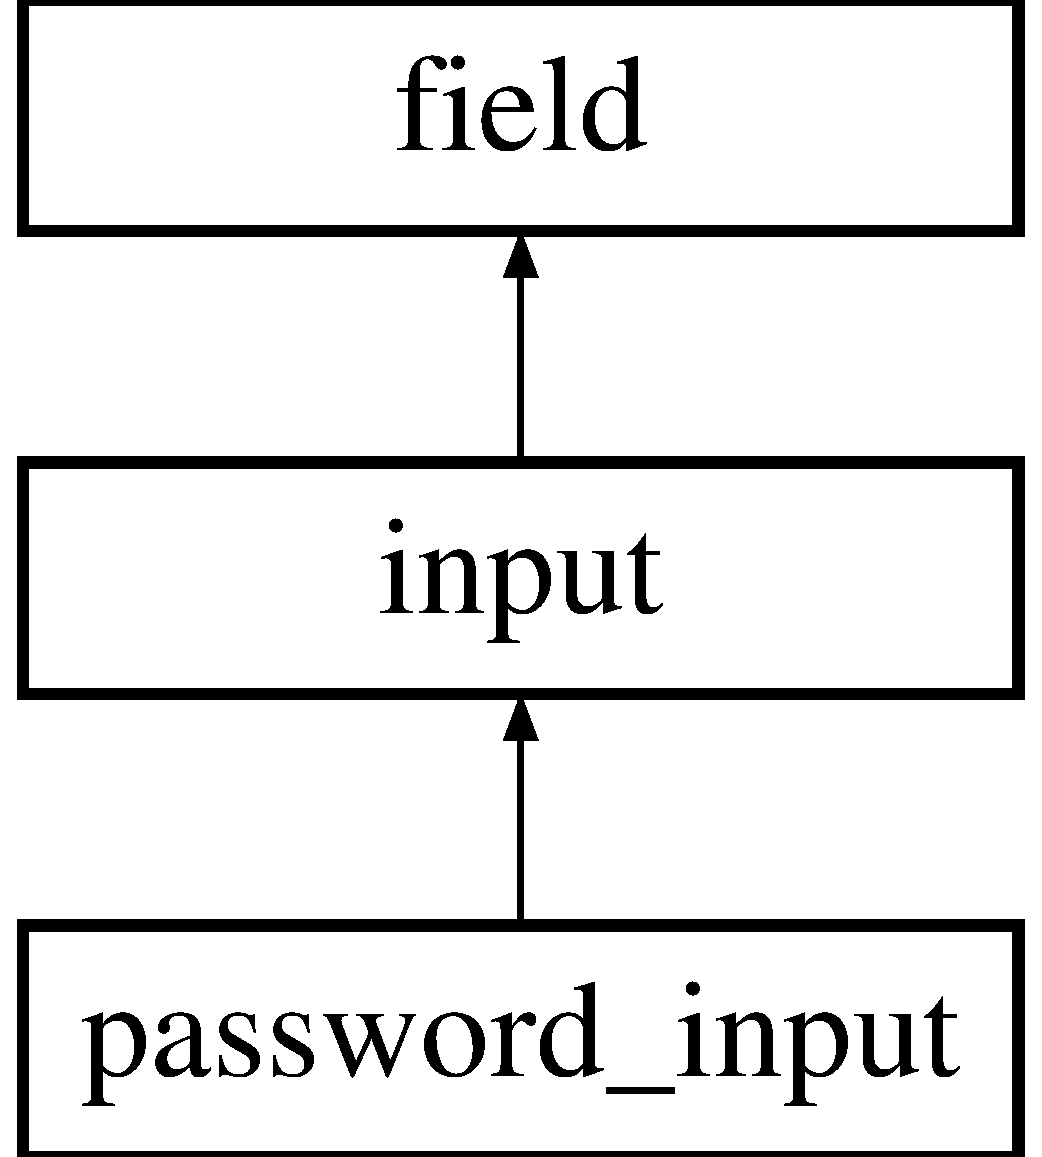
\includegraphics[height=3.000000cm]{classpassword__input}
\end{center}
\end{figure}
\subsubsection*{Public Member Functions}
\begin{DoxyCompactItemize}
\item 
\hypertarget{classpassword__input_a0cd8a0e2b305246b896256b7ad68f74d}{{\bfseries password\-\_\-input} (\$label\-\_\-text, \$name, \$value, \$required=false, \$maxlength= '', \$pattern= '', \$placeholder= '', \$sanity\-\_\-func=null, \$valid\-\_\-func=null)}\label{classpassword__input_a0cd8a0e2b305246b896256b7ad68f74d}

\end{DoxyCompactItemize}
\subsubsection*{Additional Inherited Members}


The documentation for this class was generated from the following file\-:\begin{DoxyCompactItemize}
\item 
\hyperlink{extended__inputs_8inc_8php}{extended\-\_\-inputs.\-inc.\-php}\end{DoxyCompactItemize}

\hypertarget{classprivate__get__input}{\subsection{private\-\_\-get\-\_\-input Class Reference}
\label{classprivate__get__input}\index{private\-\_\-get\-\_\-input@{private\-\_\-get\-\_\-input}}
}


This class represents a hidden input that reads its value from the \$\-\_\-\-G\-E\-T\mbox{[}\mbox{]} global array on creation, but when displaying display\-\_\-text() shows no output.  




\subsubsection{Detailed Description}
This class represents a hidden input that reads its value from the \$\-\_\-\-G\-E\-T\mbox{[}\mbox{]} global array on creation, but when displaying display\-\_\-text() shows no output. 

The documentation for this class was generated from the following file\-:\begin{DoxyCompactItemize}
\item 
\hyperlink{private__get__input_8inc_8php}{private\-\_\-get\-\_\-input.\-inc.\-php}\end{DoxyCompactItemize}

\hypertarget{classrange__input}{\subsection{range\-\_\-input Class Reference}
\label{classrange__input}\index{range\-\_\-input@{range\-\_\-input}}
}


Represents a slider element, an input with type=\char`\"{}range\char`\"{}.  


Inheritance diagram for range\-\_\-input\-:\begin{figure}[H]
\begin{center}
\leavevmode
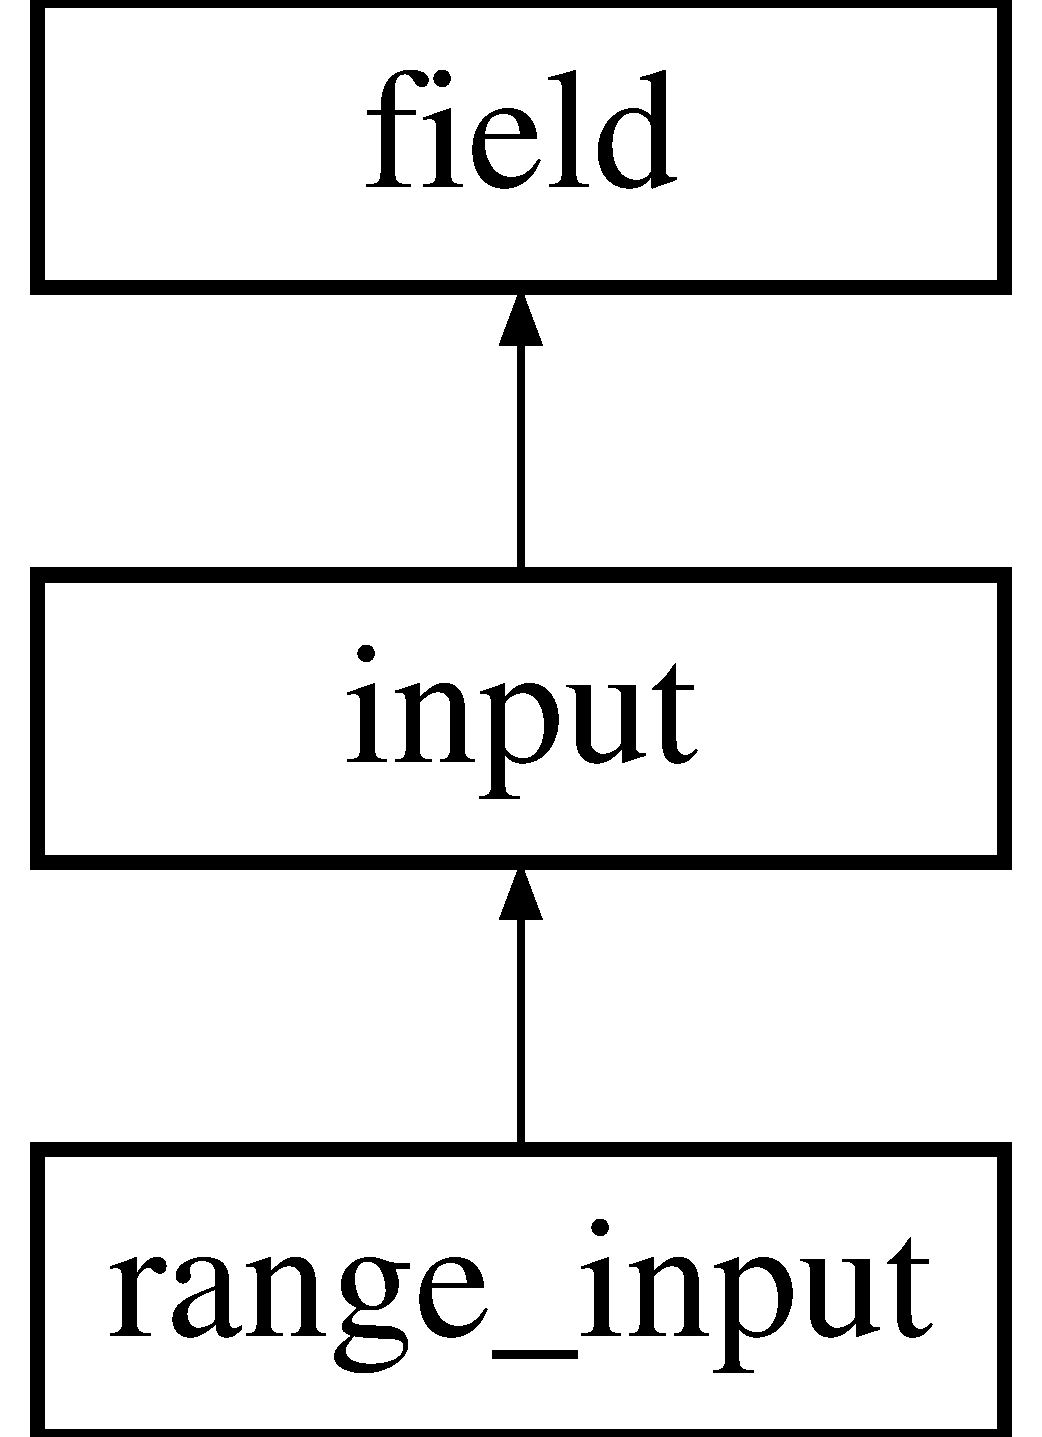
\includegraphics[height=3.000000cm]{classrange__input}
\end{center}
\end{figure}
\subsubsection*{Public Member Functions}
\begin{DoxyCompactItemize}
\item 
\hyperlink{classrange__input_a0d8240e99521fbde9c3dcd95da8aea1c}{\-\_\-\-\_\-construct} (\$label\-\_\-text, \$name, \$value, \$min= '', \$max= '', \$step= '', \$placeholder= '', \$sanity\-\_\-func=null, \$valid\-\_\-func=null)
\begin{DoxyCompactList}\small\item\em Constructor for \hyperlink{classrange__input}{range\-\_\-input}. \end{DoxyCompactList}\item 
\hyperlink{classrange__input_a84223d881e2c9279e6ca69c4957bf53e}{form} (\$errors=array())
\begin{DoxyCompactList}\small\item\em Creates H\-T\-M\-L output of a form or form part (input) from this field. \end{DoxyCompactList}\end{DoxyCompactItemize}
\subsubsection*{Public Attributes}
\begin{DoxyCompactItemize}
\item 
\hypertarget{classrange__input_ad5a0fe009154b6827fa0cb0ab2bec839}{{\bfseries \$step}}\label{classrange__input_ad5a0fe009154b6827fa0cb0ab2bec839}

\end{DoxyCompactItemize}


\subsubsection{Detailed Description}
Represents a slider element, an input with type=\char`\"{}range\char`\"{}. 



\subsubsection{Constructor \& Destructor Documentation}
\hypertarget{classrange__input_a0d8240e99521fbde9c3dcd95da8aea1c}{\index{range\-\_\-input@{range\-\_\-input}!\-\_\-\-\_\-construct@{\-\_\-\-\_\-construct}}
\index{\-\_\-\-\_\-construct@{\-\_\-\-\_\-construct}!range_input@{range\-\_\-input}}
\paragraph[{\-\_\-\-\_\-construct}]{\setlength{\rightskip}{0pt plus 5cm}range\-\_\-input\-::\-\_\-\-\_\-construct (
\begin{DoxyParamCaption}
\item[{}]{\$label\-\_\-text, }
\item[{}]{\$name, }
\item[{}]{\$value, }
\item[{}]{\$min = {\ttfamily ''}, }
\item[{}]{\$max = {\ttfamily ''}, }
\item[{}]{\$step = {\ttfamily ''}, }
\item[{}]{\$placeholder = {\ttfamily ''}, }
\item[{}]{\$sanity\-\_\-func = {\ttfamily null}, }
\item[{}]{\$valid\-\_\-func = {\ttfamily null}}
\end{DoxyParamCaption}
)}}\label{classrange__input_a0d8240e99521fbde9c3dcd95da8aea1c}


Constructor for \hyperlink{classrange__input}{range\-\_\-input}. 


\begin{DoxyParams}{Parameters}
{\em \$label\-\_\-text} & The text label for this \hyperlink{classrange__input}{range\-\_\-input}. \\
\hline
{\em \$name} & The name of this field for internal use. (i.\-e. the name attribute in the render H\-T\-M\-L and/or used in form) \\
\hline
{\em \$value} & The current value of this input. Optional. Default is ''. \\
\hline
{\em \$min} & The minium value this \hyperlink{classnumber__input}{number\-\_\-input} allows, used in validation and H\-T\-M\-L5 min attribute. Optional. If not set, or set to '', this attribute is ignored. \\
\hline
{\em \$max} & The maximum value this \hyperlink{classnumber__input}{number\-\_\-input} allows, used in validation and H\-T\-M\-L5 max attribute. Optional. If not set, or set to '', this attribute is ignored. \\
\hline
{\em \$step} & This is the H\-T\-M\-L5 step attribute. Optional. If not set, or set to '', this attribute is ignored. \\
\hline
{\em \$placeholder} & This is used for the H\-T\-M\-L5 placeholder attribute. Optional. Default is false. \\
\hline
{\em \$sanity\-\_\-func} & Optional function for sanitization. Defualt is null. \\
\hline
{\em \$valid\-\_\-func} & Optional function for validation. Default is null. \\
\hline
\end{DoxyParams}


\subsubsection{Member Function Documentation}
\hypertarget{classrange__input_a84223d881e2c9279e6ca69c4957bf53e}{\index{range\-\_\-input@{range\-\_\-input}!form@{form}}
\index{form@{form}!range_input@{range\-\_\-input}}
\paragraph[{form}]{\setlength{\rightskip}{0pt plus 5cm}range\-\_\-input\-::form (
\begin{DoxyParamCaption}
\item[{}]{\$errors = {\ttfamily array()}}
\end{DoxyParamCaption}
)}}\label{classrange__input_a84223d881e2c9279e6ca69c4957bf53e}


Creates H\-T\-M\-L output of a form or form part (input) from this field. 


\begin{DoxyParams}[1]{Parameters}
array & {\em \$errors} & The errors that have been found, should be used to add error styles or display error messages. \\
\hline
\end{DoxyParams}
\begin{DoxyReturn}{Returns}
an associated array with two element 'html' =$>$ the H\-T\-M\-L of this object 'js' =$>$ the Javascript of this object 
\end{DoxyReturn}


Implements \hyperlink{interfacefield_a1b51c4b8b01f77a26eda359e1fc0fb4c}{field}.



The documentation for this class was generated from the following file\-:\begin{DoxyCompactItemize}
\item 
\hyperlink{extended__inputs_8inc_8php}{extended\-\_\-inputs.\-inc.\-php}\end{DoxyCompactItemize}

\hypertarget{classtel__input}{\subsection{tel\-\_\-input Class Reference}
\label{classtel__input}\index{tel\-\_\-input@{tel\-\_\-input}}
}


This represents a telephone number input, has regex sanitization and validation to ensure valid format for phone 7 or 10 digit phone number.  


Inheritance diagram for tel\-\_\-input\-:\begin{figure}[H]
\begin{center}
\leavevmode
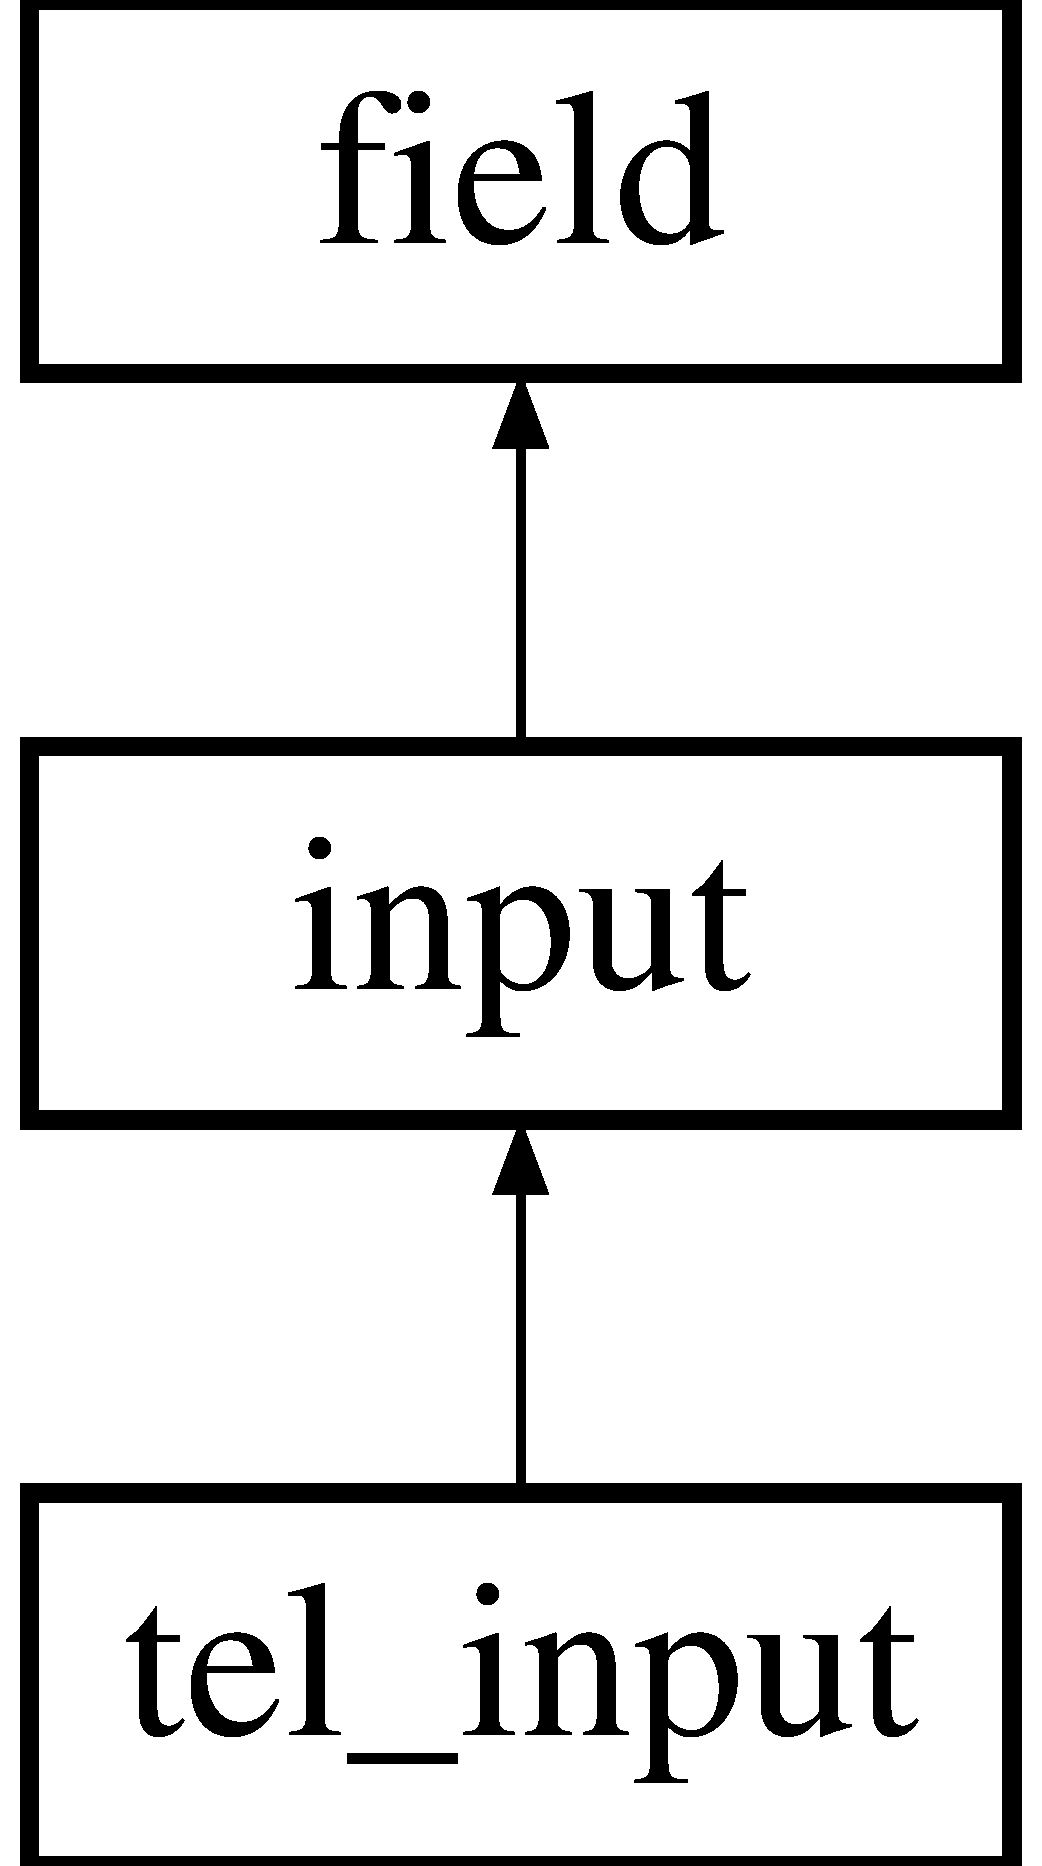
\includegraphics[height=3.000000cm]{classtel__input}
\end{center}
\end{figure}
\subsubsection*{Public Member Functions}
\begin{DoxyCompactItemize}
\item 
\hyperlink{classtel__input_aac420f3bfa98941083dbb0e2c54b19ab}{\-\_\-\-\_\-construct} (\$label\-\_\-text, \$name, \$value= '', \$required=false, \$placeholder=\char`\"{}(X\-X\-X) X\-X\-X-\/X\-X\-X\-X\char`\"{}, \$sanity\-\_\-func=null, \$valid\-\_\-func=null)
\begin{DoxyCompactList}\small\item\em Constructor for \hyperlink{classtel__input}{tel\-\_\-input} object. \end{DoxyCompactList}\end{DoxyCompactItemize}
\subsubsection*{Additional Inherited Members}


\subsubsection{Detailed Description}
This represents a telephone number input, has regex sanitization and validation to ensure valid format for phone 7 or 10 digit phone number. 

\subsubsection{Constructor \& Destructor Documentation}
\hypertarget{classtel__input_aac420f3bfa98941083dbb0e2c54b19ab}{\index{tel\-\_\-input@{tel\-\_\-input}!\-\_\-\-\_\-construct@{\-\_\-\-\_\-construct}}
\index{\-\_\-\-\_\-construct@{\-\_\-\-\_\-construct}!tel_input@{tel\-\_\-input}}
\paragraph[{\-\_\-\-\_\-construct}]{\setlength{\rightskip}{0pt plus 5cm}tel\-\_\-input\-::\-\_\-\-\_\-construct (
\begin{DoxyParamCaption}
\item[{}]{\$label\-\_\-text, }
\item[{}]{\$name, }
\item[{}]{\$value = {\ttfamily ''}, }
\item[{}]{\$required = {\ttfamily false}, }
\item[{}]{\$placeholder = {\ttfamily \char`\"{}(XXX)~XXX-\/XXXX\char`\"{}}, }
\item[{}]{\$sanity\-\_\-func = {\ttfamily null}, }
\item[{}]{\$valid\-\_\-func = {\ttfamily null}}
\end{DoxyParamCaption}
)}}\label{classtel__input_aac420f3bfa98941083dbb0e2c54b19ab}


Constructor for \hyperlink{classtel__input}{tel\-\_\-input} object. 


\begin{DoxyParams}{Parameters}
{\em \$label\-\_\-text} & The text label for this \hyperlink{classtel__input}{tel\-\_\-input}. \\
\hline
{\em \$name} & The name of this field for internal use. (i.\-e. the name attribute in the render H\-T\-M\-L and/or used in form) \\
\hline
{\em \$value} & The current value of this input. Optional. Default is ''. \\
\hline
{\em \$required} & Weather or not the user is required to enter this field. This effects both H\-T\-M\-L5 element and validation. Optional. Default is false. \\
\hline
{\em \$placeholder} & This is used for the H\-T\-M\-L5 placeholder attribute. Optional. Default is false. \\
\hline
{\em \$sanity\-\_\-func} & Optional function for sanitization. Defualt is null. \\
\hline
{\em \$valid\-\_\-func} & Optional function for validation. Default is null. \\
\hline
\end{DoxyParams}


The documentation for this class was generated from the following file\-:\begin{DoxyCompactItemize}
\item 
\hyperlink{extended__inputs_8inc_8php}{extended\-\_\-inputs.\-inc.\-php}\end{DoxyCompactItemize}

\hypertarget{classtext__input}{\subsection{text\-\_\-input Class Reference}
\label{classtext__input}\index{text\-\_\-input@{text\-\_\-input}}
}


convience function for creating text inputs  


Inheritance diagram for text\-\_\-input\-:\begin{figure}[H]
\begin{center}
\leavevmode
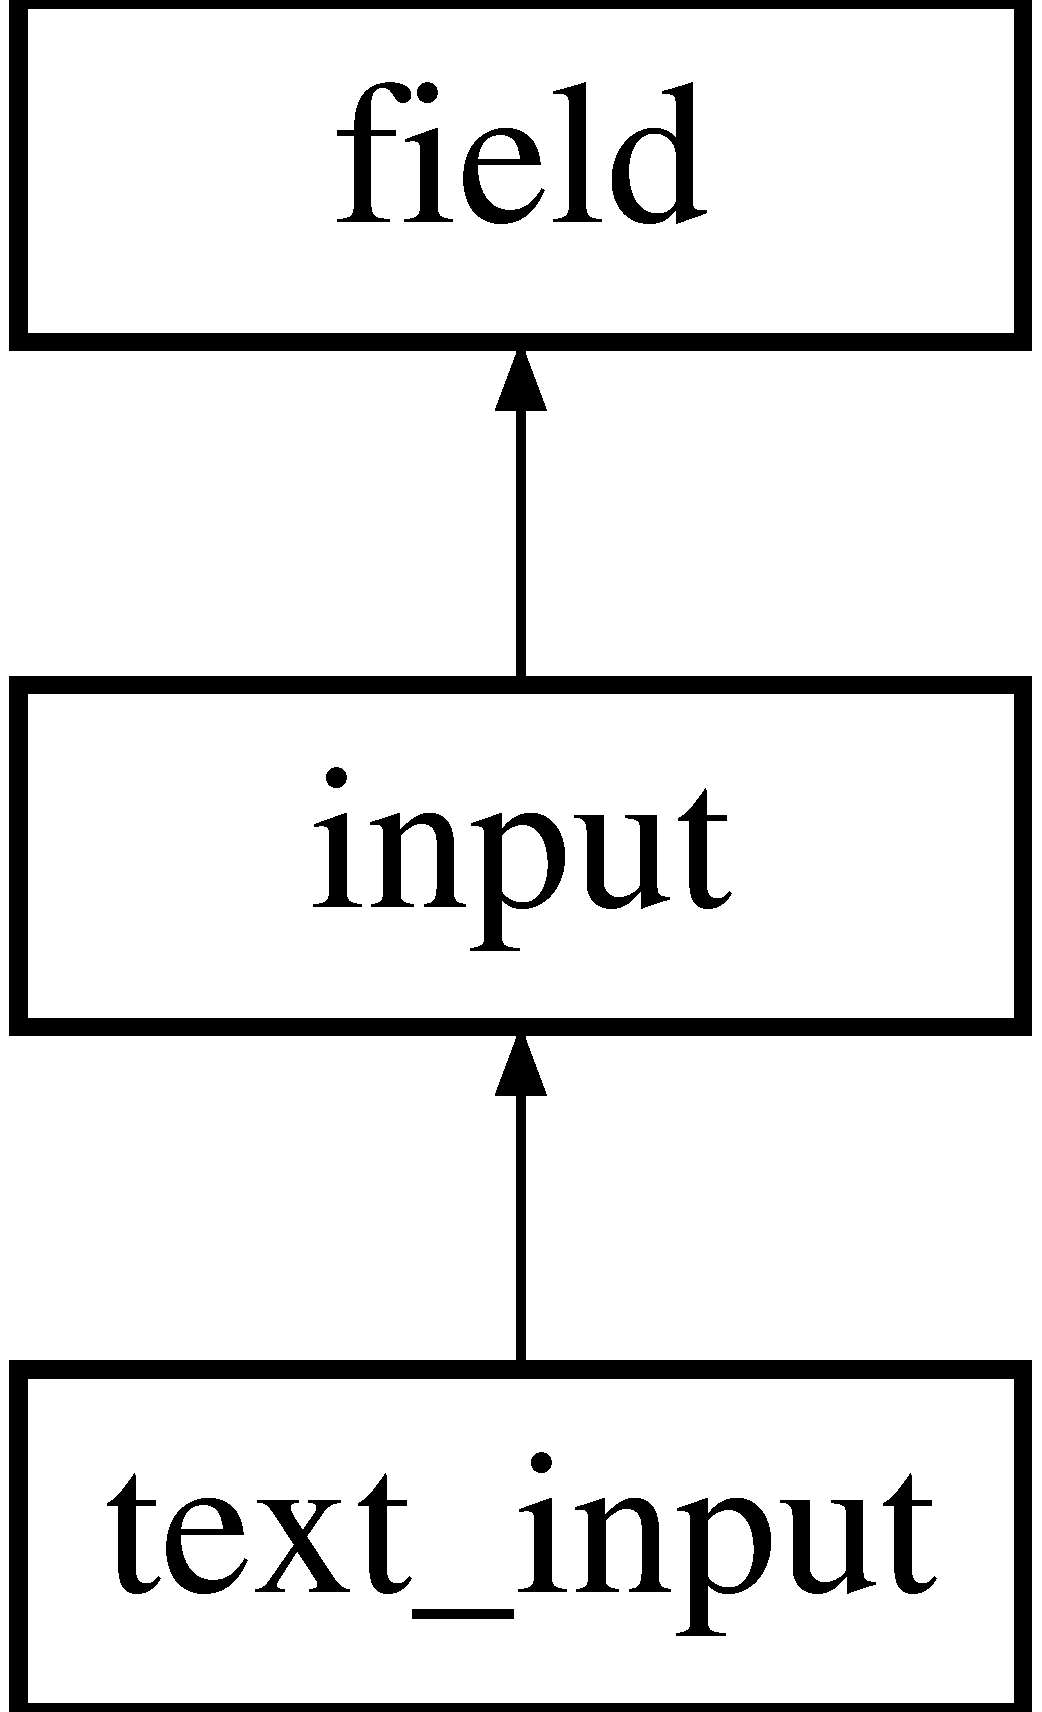
\includegraphics[height=3.000000cm]{classtext__input}
\end{center}
\end{figure}
\subsubsection*{Public Member Functions}
\begin{DoxyCompactItemize}
\item 
\hypertarget{classtext__input_a5099af7bcf7d4cb5ad348e5662ed9de4}{{\bfseries \-\_\-\-\_\-construct} (\$label\-\_\-text, \$name, \$value, \$required=false, \$maxlength= '', \$pattern= '', \$placeholder= '', \$sanity\-\_\-func=null, \$valid\-\_\-func=null)}\label{classtext__input_a5099af7bcf7d4cb5ad348e5662ed9de4}

\end{DoxyCompactItemize}
\subsubsection*{Additional Inherited Members}


\subsubsection{Detailed Description}
convience function for creating text inputs 



The documentation for this class was generated from the following file\-:\begin{DoxyCompactItemize}
\item 
\hyperlink{extended__inputs_8inc_8php}{extended\-\_\-inputs.\-inc.\-php}\end{DoxyCompactItemize}

\hypertarget{classtextarea}{\subsection{textarea Class Reference}
\label{classtextarea}\index{textarea@{textarea}}
}


Descibes a textarea, it's sanitzation and validation.  


Inheritance diagram for textarea\-:\begin{figure}[H]
\begin{center}
\leavevmode
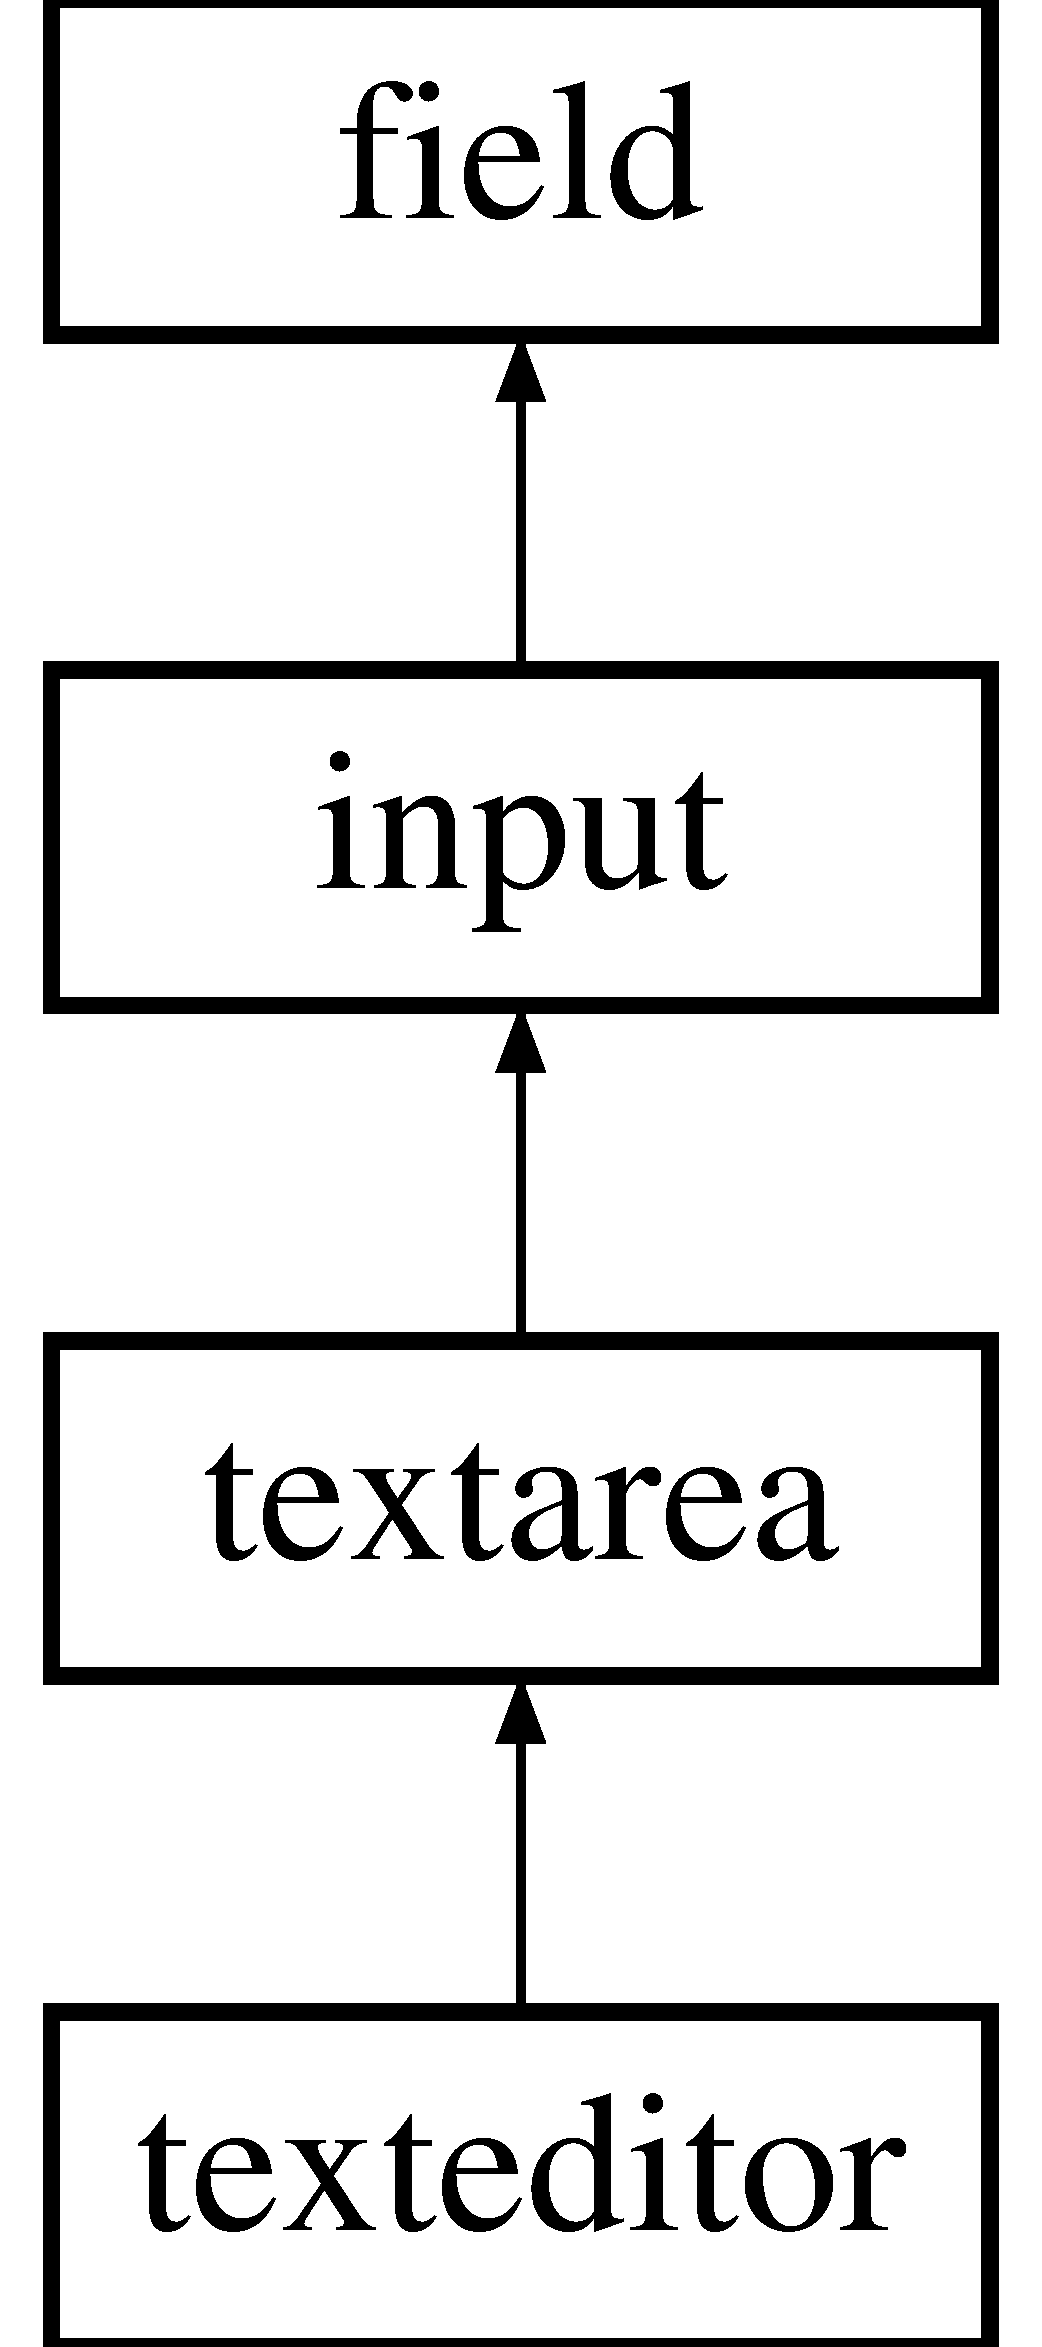
\includegraphics[height=4.000000cm]{classtextarea}
\end{center}
\end{figure}
\subsubsection*{Public Member Functions}
\begin{DoxyCompactItemize}
\item 
\hyperlink{classtextarea_a711ac3a17f0e150fd9a0c73c7633e1a1}{textarea} (\$label\-\_\-text, \$name, \$value= '', \$required=false, \$maxlength= '', \$sanity\-\_\-func=null, \$valid\-\_\-func=null)
\begin{DoxyCompactList}\small\item\em Constructor, creates a text\-\_\-area object. \end{DoxyCompactList}\item 
\hyperlink{classtextarea_a3e3d02a7c0ff76c86f6b987e1193ca6a}{form} (\$errors=array())
\begin{DoxyCompactList}\small\item\em Generates the html for the textarea for inclusion in a form. \end{DoxyCompactList}\end{DoxyCompactItemize}
\subsubsection*{Additional Inherited Members}


\subsubsection{Detailed Description}
Descibes a textarea, it's sanitzation and validation. 

\subsubsection{Member Function Documentation}
\hypertarget{classtextarea_a3e3d02a7c0ff76c86f6b987e1193ca6a}{\index{textarea@{textarea}!form@{form}}
\index{form@{form}!textarea@{textarea}}
\paragraph[{form}]{\setlength{\rightskip}{0pt plus 5cm}textarea\-::form (
\begin{DoxyParamCaption}
\item[{}]{\$errors = {\ttfamily array()}}
\end{DoxyParamCaption}
)}}\label{classtextarea_a3e3d02a7c0ff76c86f6b987e1193ca6a}


Generates the html for the textarea for inclusion in a form. 


\begin{DoxyParams}[1]{Parameters}
array & {\em \$errors} & an accoiated array errors. If the field name appears in errors, the field's label will be a class of error. \\
\hline
\end{DoxyParams}
\begin{DoxyReturn}{Returns}
array with two elements 'html' the H\-T\-M\-L of the input field and 'js' any Java\-Script that would assoicated with it (empty for basic input types at this time). 
\end{DoxyReturn}


Implements \hyperlink{interfacefield_a1b51c4b8b01f77a26eda359e1fc0fb4c}{field}.

\hypertarget{classtextarea_a711ac3a17f0e150fd9a0c73c7633e1a1}{\index{textarea@{textarea}!textarea@{textarea}}
\index{textarea@{textarea}!textarea@{textarea}}
\paragraph[{textarea}]{\setlength{\rightskip}{0pt plus 5cm}textarea\-::textarea (
\begin{DoxyParamCaption}
\item[{}]{\$label\-\_\-text, }
\item[{}]{\$name, }
\item[{}]{\$value = {\ttfamily ''}, }
\item[{}]{\$required = {\ttfamily false}, }
\item[{}]{\$maxlength = {\ttfamily ''}, }
\item[{}]{\$sanity\-\_\-func = {\ttfamily null}, }
\item[{}]{\$valid\-\_\-func = {\ttfamily null}}
\end{DoxyParamCaption}
)}}\label{classtextarea_a711ac3a17f0e150fd9a0c73c7633e1a1}


Constructor, creates a text\-\_\-area object. 


\begin{DoxyParams}[1]{Parameters}
string & {\em \$label\-\_\-text} & The text label on the form field. \\
\hline
string & {\em \$name} & The name of the field used to identify this field in the database, and in the form. \\
\hline
mixed & {\em \$value} & The current value of the field. \\
\hline
bool & {\em \$required} & Boolean value, weather or not the user is required to enter a value for the field. \\
\hline
mixed & {\em \$maxlength} & The maximum characters this field's value can have, and still be valid. null or empty string will make this be ignored. \\
\hline
mixed & {\em \$sanity\-\_\-func} & A function run on this element to sanitize it, if null will use default sanitation and validation using attributes above. \\
\hline
mixed & {\em \$valid\-\_\-func} & A function run on this element to validate it, if null will use default sanitation and validation using attributes above. \\
\hline
\end{DoxyParams}


The documentation for this class was generated from the following file\-:\begin{DoxyCompactItemize}
\item 
\hyperlink{textarea_8inc_8php}{textarea.\-inc.\-php}\end{DoxyCompactItemize}

\hypertarget{classtexteditor}{\subsection{texteditor Class Reference}
\label{classtexteditor}\index{texteditor@{texteditor}}
}


This is a form element wrapping the testarea with javascript to turn it into a rich text editor.  


Inheritance diagram for texteditor\-:\begin{figure}[H]
\begin{center}
\leavevmode
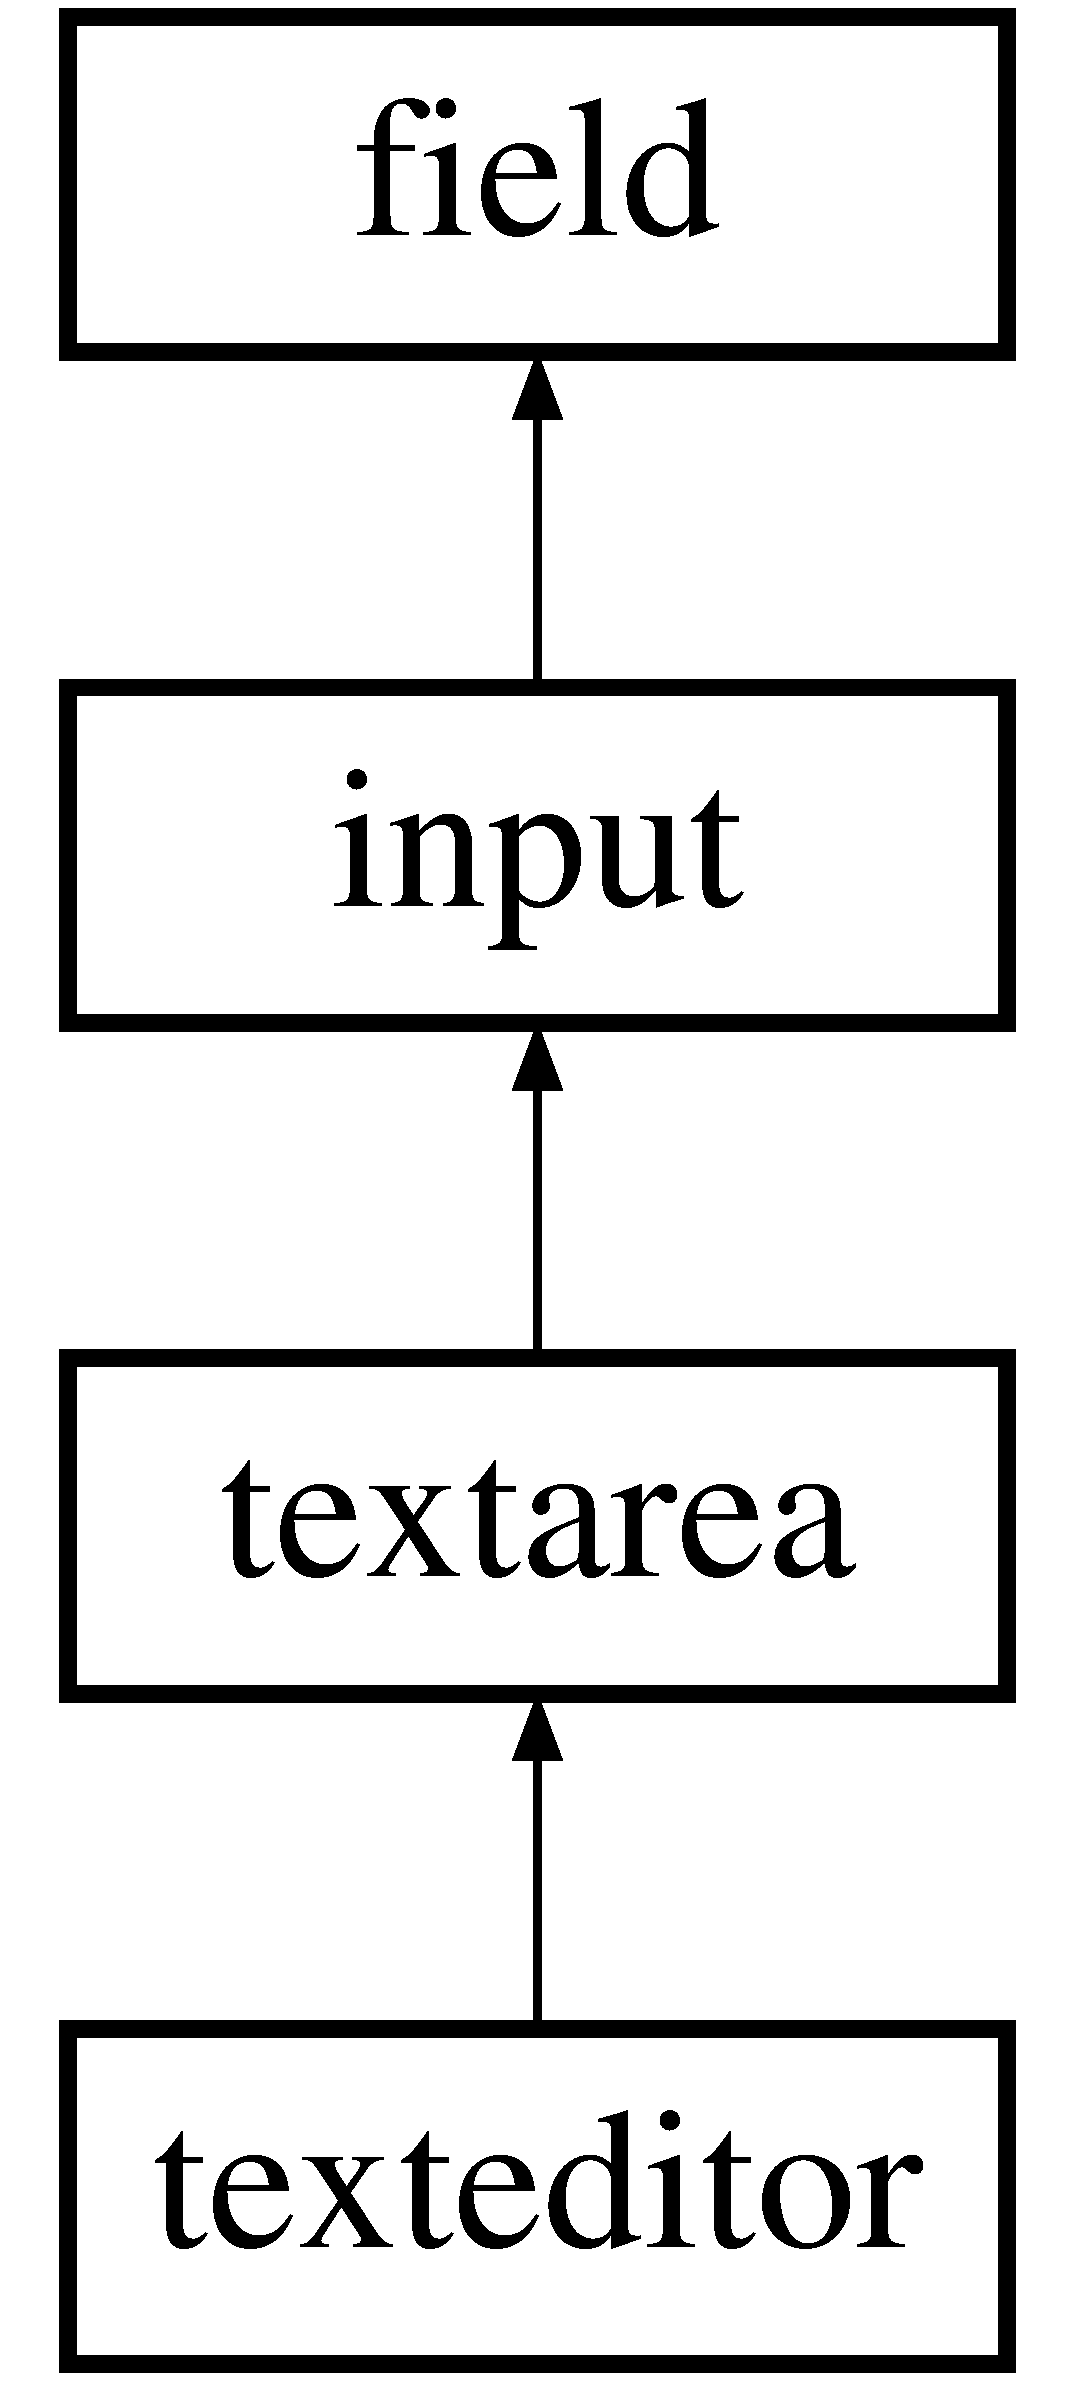
\includegraphics[height=4.000000cm]{classtexteditor}
\end{center}
\end{figure}
\subsubsection*{Public Member Functions}
\begin{DoxyCompactItemize}
\item 
\hypertarget{classtexteditor_a6ecfa4454b5b96286732f0f503e6485b}{{\bfseries texteditor} (\$label\-\_\-text, \$name, \$value= '', \$required=false, \$maxlength= '', \$sanity\-\_\-func=null, \$valid\-\_\-func=null)}\label{classtexteditor_a6ecfa4454b5b96286732f0f503e6485b}

\item 
\hyperlink{classtexteditor_a129b929db008ec11f4a683f542787c74}{form} (\$errors)
\begin{DoxyCompactList}\small\item\em Creates H\-T\-M\-L output of a form or form part (input) from this field. \end{DoxyCompactList}\end{DoxyCompactItemize}
\subsubsection*{Additional Inherited Members}


\subsubsection{Detailed Description}
This is a form element wrapping the testarea with javascript to turn it into a rich text editor. 

\subsubsection{Member Function Documentation}
\hypertarget{classtexteditor_a129b929db008ec11f4a683f542787c74}{\index{texteditor@{texteditor}!form@{form}}
\index{form@{form}!texteditor@{texteditor}}
\paragraph[{form}]{\setlength{\rightskip}{0pt plus 5cm}texteditor\-::form (
\begin{DoxyParamCaption}
\item[{}]{\$errors}
\end{DoxyParamCaption}
)}}\label{classtexteditor_a129b929db008ec11f4a683f542787c74}


Creates H\-T\-M\-L output of a form or form part (input) from this field. 


\begin{DoxyParams}[1]{Parameters}
array & {\em \$errors} & The errors that have been found, should be used to add error styles or display error messages. \\
\hline
\end{DoxyParams}
\begin{DoxyReturn}{Returns}
an associated array with two element 'html' =$>$ the H\-T\-M\-L of this object 'js' =$>$ the Javascript of this object 
\end{DoxyReturn}


Implements \hyperlink{interfacefield_a1b51c4b8b01f77a26eda359e1fc0fb4c}{field}.



The documentation for this class was generated from the following file\-:\begin{DoxyCompactItemize}
\item 
\hyperlink{texteditor_8inc_8php}{texteditor.\-inc.\-php}\end{DoxyCompactItemize}

\hypertarget{classzip__input}{\subsection{zip\-\_\-input Class Reference}
\label{classzip__input}\index{zip\-\_\-input@{zip\-\_\-input}}
}


This convience class creates a text input with validation for long or short form U\-S zip codes.  


Inheritance diagram for zip\-\_\-input\-:\begin{figure}[H]
\begin{center}
\leavevmode
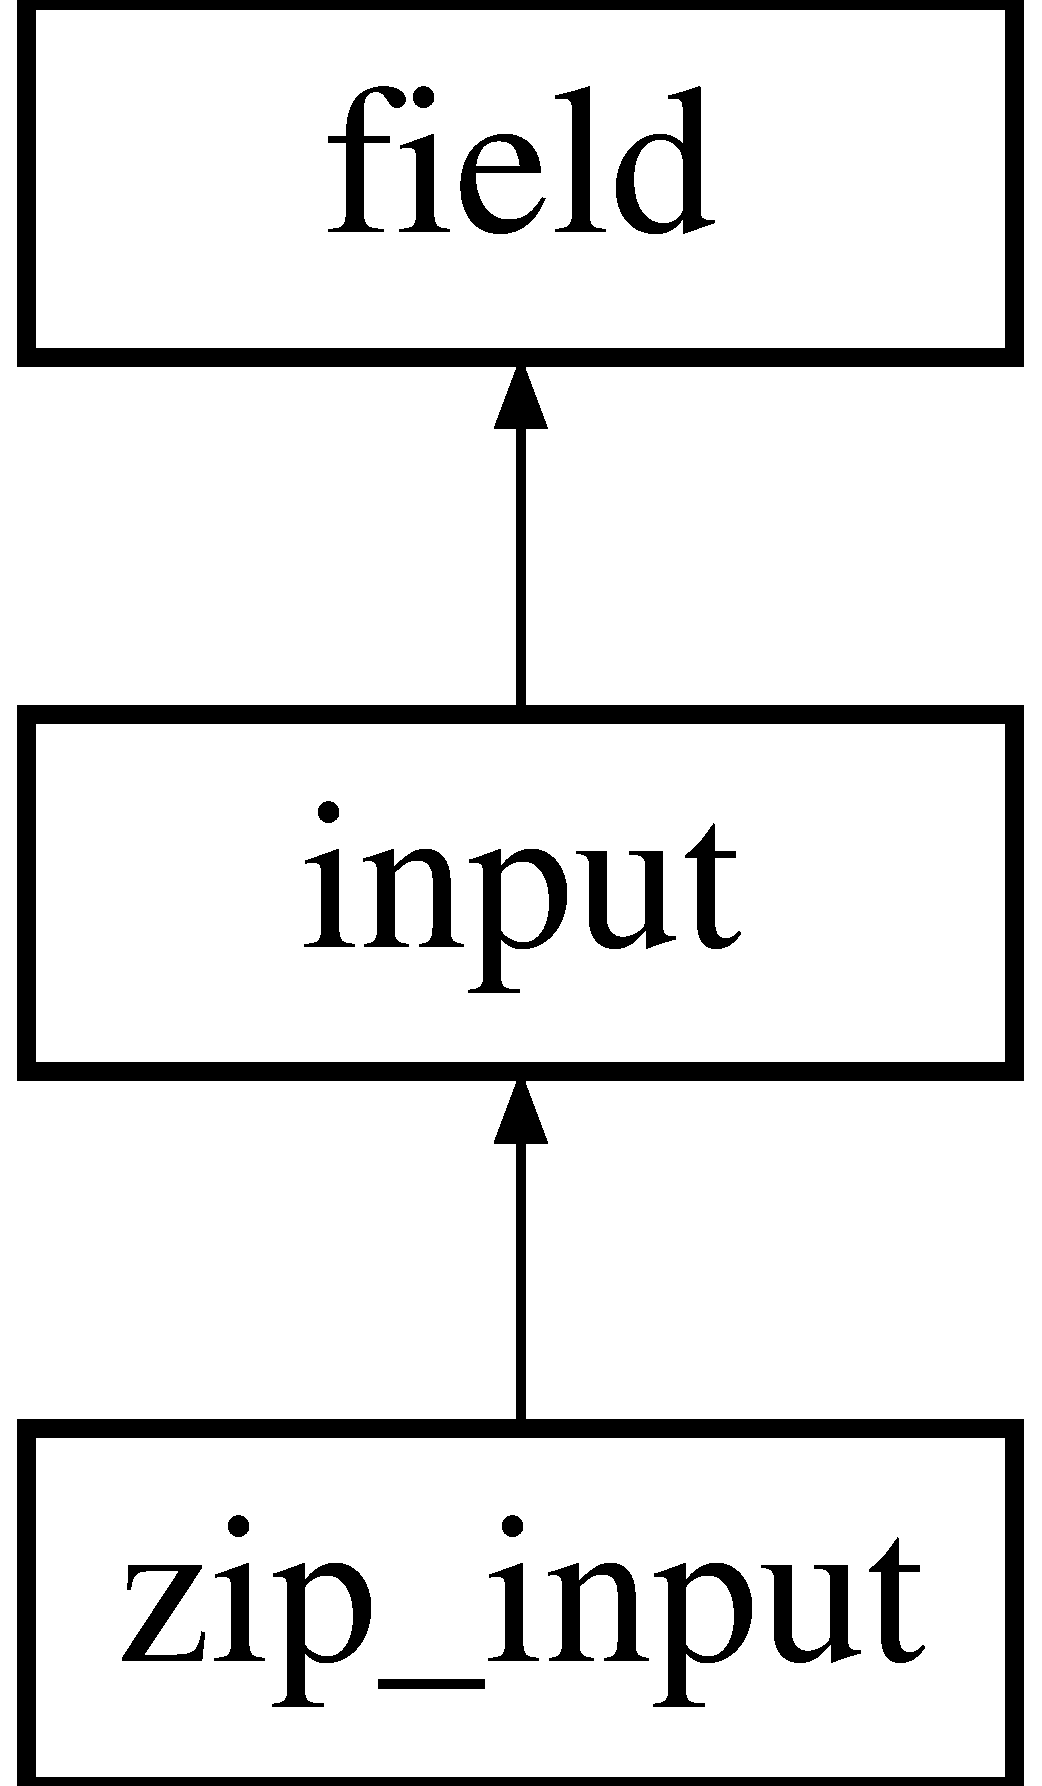
\includegraphics[height=3.000000cm]{classzip__input}
\end{center}
\end{figure}
\subsubsection*{Public Member Functions}
\begin{DoxyCompactItemize}
\item 
\hyperlink{classzip__input_a1e3ec25aa5cac0d6da454409efbceb9b}{\-\_\-\-\_\-construct} (\$label\-\_\-text, \$name, \$value, \$required=false, \$placeholder=\char`\"{}X\-X\-X\-X\-X\mbox{[}-\/X\-X\-X\-X\mbox{]}\char`\"{}, \$sanity\-\_\-func=null, \$valid\-\_\-func=null)
\begin{DoxyCompactList}\small\item\em Constructor for \hyperlink{classzip__input}{zip\-\_\-input}. \end{DoxyCompactList}\end{DoxyCompactItemize}
\subsubsection*{Additional Inherited Members}


\subsubsection{Detailed Description}
This convience class creates a text input with validation for long or short form U\-S zip codes. 

\subsubsection{Constructor \& Destructor Documentation}
\hypertarget{classzip__input_a1e3ec25aa5cac0d6da454409efbceb9b}{\index{zip\-\_\-input@{zip\-\_\-input}!\-\_\-\-\_\-construct@{\-\_\-\-\_\-construct}}
\index{\-\_\-\-\_\-construct@{\-\_\-\-\_\-construct}!zip_input@{zip\-\_\-input}}
\paragraph[{\-\_\-\-\_\-construct}]{\setlength{\rightskip}{0pt plus 5cm}zip\-\_\-input\-::\-\_\-\-\_\-construct (
\begin{DoxyParamCaption}
\item[{}]{\$label\-\_\-text, }
\item[{}]{\$name, }
\item[{}]{\$value, }
\item[{}]{\$required = {\ttfamily false}, }
\item[{}]{\$placeholder = {\ttfamily \char`\"{}XXXXX\mbox{[}-\/XXXX\mbox{]}\char`\"{}}, }
\item[{}]{\$sanity\-\_\-func = {\ttfamily null}, }
\item[{}]{\$valid\-\_\-func = {\ttfamily null}}
\end{DoxyParamCaption}
)}}\label{classzip__input_a1e3ec25aa5cac0d6da454409efbceb9b}


Constructor for \hyperlink{classzip__input}{zip\-\_\-input}. 


\begin{DoxyParams}{Parameters}
{\em \$label\-\_\-text} & The text label for this \hyperlink{classzip__input}{zip\-\_\-input}. \\
\hline
{\em \$name} & The name of this field for internal use. (i.\-e. the name attribute in the render H\-T\-M\-L and/or used in form) \\
\hline
{\em \$value} & The current value of this input. Optional. Default is ''. \\
\hline
{\em \$required} & Weather or not the user is required to enter this field. This effects both H\-T\-M\-L5 element and validation. Optional. Default is false. \\
\hline
{\em \$placeholder} & This is used for the H\-T\-M\-L5 placeholder attribute. Optional. Default is false. \\
\hline
{\em \$sanity\-\_\-func} & Optional function for sanitization. Defualt is null. \\
\hline
{\em \$valid\-\_\-func} & Optional function for validation. Default is null. \\
\hline
\end{DoxyParams}


The documentation for this class was generated from the following file\-:\begin{DoxyCompactItemize}
\item 
\hyperlink{extended__inputs_8inc_8php}{extended\-\_\-inputs.\-inc.\-php}\end{DoxyCompactItemize}

\section{File Documentation}
\hypertarget{api_8php}{\subsection{api.\-php File Reference}
\label{api_8php}\index{api.\-php@{api.\-php}}
}


This file defines the api for form building.  


\subsubsection*{Variables}
\begin{DoxyCompactItemize}
\item 
\hypertarget{api_8php_a03b3894f94a4a13f6de58cc6150584f3}{{\bfseries \$builder} = new \hyperlink{classbuilder__form}{builder\-\_\-form}()}\label{api_8php_a03b3894f94a4a13f6de58cc6150584f3}

\item 
{\bfseries \$input\-\_\-whitelist}
\item 
{\bfseries \$required\-\_\-values}
\item 
\hypertarget{api_8php_a48d91bd968259d1544bb78a8b0ffe541}{{\bfseries \$form\-\_\-names} = array()}\label{api_8php_a48d91bd968259d1544bb78a8b0ffe541}

\item 
\hypertarget{api_8php_a172a3ce731ebb53eb004cf719f977d6d}{{\bfseries \$stmnt} = \$db-\/$>$prepare('select distinct name from \hyperlink{classforms}{forms}')}\label{api_8php_a172a3ce731ebb53eb004cf719f977d6d}

\item 
if(isset(\$\-\_\-\-R\-E\-Q\-U\-E\-S\-T\mbox{[}'type'\mbox{]})\&\&in\-\_\-array(\$\-\_\-\-R\-E\-Q\-U\-E\-S\-T\mbox{[}'type'\mbox{]}, \\*
\$input\-\_\-whitelist)) else if(!isset(\$\-\_\-\-R\-E\-Q\-U\-E\-S\-T\mbox{[}'type'\mbox{]})) {\bfseries else}
\end{DoxyCompactItemize}


\subsubsection{Detailed Description}
This file defines the api for form building. \begin{DoxyAuthor}{Author}
Jeremy Streich 
\end{DoxyAuthor}


\subsubsection{Variable Documentation}
\hypertarget{api_8php_a8f899b4769ac4dac9b39bf08a09320bb}{\index{api.\-php@{api.\-php}!\$input\-\_\-whitelist@{\$input\-\_\-whitelist}}
\index{\$input\-\_\-whitelist@{\$input\-\_\-whitelist}!api.php@{api.\-php}}
\paragraph[{\$input\-\_\-whitelist}]{\setlength{\rightskip}{0pt plus 5cm}\$input\-\_\-whitelist}}\label{api_8php_a8f899b4769ac4dac9b39bf08a09320bb}
{\bfseries Initial value\-:}
\begin{DoxyCode}
= array
  (
    \textcolor{stringliteral}{'input'},
    \textcolor{stringliteral}{'color\_input'},
    \textcolor{stringliteral}{'datalist\_input'},
    \textcolor{stringliteral}{'date\_input'},
    \textcolor{stringliteral}{'email\_input'},
    \textcolor{stringliteral}{'hidden\_input'},
    \textcolor{stringliteral}{'input\_group'},
    \textcolor{stringliteral}{'number\_input'},
    \textcolor{stringliteral}{'password\_input'},
    \textcolor{stringliteral}{'range\_input'},
    \textcolor{stringliteral}{'tel\_input'},
    \textcolor{stringliteral}{'text\_input'},
    \textcolor{stringliteral}{'textarea'},
    \textcolor{stringliteral}{'zip\_input'},
    \textcolor{stringliteral}{'get\_input'},
    \textcolor{stringliteral}{'texteditor'}
  )
\end{DoxyCode}
\hypertarget{api_8php_af377fd4ccbb6ba49860aaed32716e805}{\index{api.\-php@{api.\-php}!\$required\-\_\-values@{\$required\-\_\-values}}
\index{\$required\-\_\-values@{\$required\-\_\-values}!api.php@{api.\-php}}
\paragraph[{\$required\-\_\-values}]{\setlength{\rightskip}{0pt plus 5cm}\$required\-\_\-values}}\label{api_8php_af377fd4ccbb6ba49860aaed32716e805}
{\bfseries Initial value\-:}
\begin{DoxyCode}
= array
  (
    \textcolor{stringliteral}{'yes'} => \textcolor{keyword}{true},
    \textcolor{stringliteral}{'no'} => \textcolor{keyword}{false},
    \textcolor{charliteral}{'y'} => \textcolor{keyword}{true},
    \textcolor{charliteral}{'n'} => \textcolor{keyword}{false},
    \textcolor{charliteral}{'1'} => \textcolor{keyword}{true},
    \textcolor{charliteral}{'0'} => \textcolor{keyword}{false},
    \textcolor{stringliteral}{'on'} => \textcolor{keyword}{true},
    \textcolor{stringliteral}{'off'} => \textcolor{keyword}{false},
    \textcolor{keyword}{true} => \textcolor{keyword}{true},
    \textcolor{keyword}{false} => \textcolor{keyword}{false}
  )
\end{DoxyCode}
\hypertarget{api_8php_a67ca52de78eee3b8906311c86f3d8a7e}{\index{api.\-php@{api.\-php}!else@{else}}
\index{else@{else}!api.php@{api.\-php}}
\paragraph[{else}]{\setlength{\rightskip}{0pt plus 5cm}if (!isset(\$\-\_\-\-R\-E\-Q\-U\-E\-S\-T\mbox{[}'required'\mbox{]})) else if (array\-\_\-key\-\_\-exists(\$\-\_\-\-R\-E\-Q\-U\-E\-S\-T\mbox{[}'required'\mbox{]}, \$required\-\_\-values)) else}}\label{api_8php_a67ca52de78eee3b8906311c86f3d8a7e}
{\bfseries Initial value\-:}
\begin{DoxyCode}
\{
    http\_response\_code(201)
\end{DoxyCode}

\hypertarget{crud_8inc_8php}{\subsection{crud.\-inc.\-php File Reference}
\label{crud_8inc_8php}\index{crud.\-inc.\-php@{crud.\-inc.\-php}}
}


Contains the interface for crud.  


\subsubsection*{Classes}
\begin{DoxyCompactItemize}
\item 
interface \hyperlink{interfacecrud}{crud}
\begin{DoxyCompactList}\small\item\em Describes an object that knows how to Create, Read, Update and Delete iteself. \end{DoxyCompactList}\end{DoxyCompactItemize}


\subsubsection{Detailed Description}
Contains the interface for crud. 
\hypertarget{database__form_8inc_8php}{\subsection{database\-\_\-form.\-inc.\-php File Reference}
\label{database__form_8inc_8php}\index{database\-\_\-form.\-inc.\-php@{database\-\_\-form.\-inc.\-php}}
}
\subsubsection*{Classes}
\begin{DoxyCompactItemize}
\item 
class \hyperlink{classdatabase__form}{database\-\_\-form}
\begin{DoxyCompactList}\small\item\em This class allows the both the structure and the data for this form to be written out to a database. \end{DoxyCompactList}\end{DoxyCompactItemize}
\subsubsection*{Variables}
\begin{DoxyCompactItemize}
\item 
\hypertarget{database__form_8inc_8php_ab932cfce57ae4999624324a6aa42b52f}{const {\bfseries P\-R\-E\-\_\-\-C\-R\-E\-A\-T\-E} 13}\label{database__form_8inc_8php_ab932cfce57ae4999624324a6aa42b52f}

\item 
\hypertarget{database__form_8inc_8php_ad4fd956648dde9018d8d3eaf36fdeb40}{const {\bfseries P\-O\-S\-T\-\_\-\-C\-R\-E\-A\-T\-E} 14}\label{database__form_8inc_8php_ad4fd956648dde9018d8d3eaf36fdeb40}

\item 
\hypertarget{database__form_8inc_8php_a361873e4d0f0296f73a3665203809e37}{const {\bfseries P\-R\-E\-\_\-\-R\-E\-A\-D} 15}\label{database__form_8inc_8php_a361873e4d0f0296f73a3665203809e37}

\item 
\hypertarget{database__form_8inc_8php_a19915709359fcf522fa42e08366b0d12}{const {\bfseries P\-O\-S\-T\-\_\-\-R\-E\-A\-D} 16}\label{database__form_8inc_8php_a19915709359fcf522fa42e08366b0d12}

\item 
\hypertarget{database__form_8inc_8php_a2bbbf801874089634adaf45b56975031}{const {\bfseries P\-R\-E\-\_\-\-U\-P\-D\-A\-T\-E} 17}\label{database__form_8inc_8php_a2bbbf801874089634adaf45b56975031}

\item 
\hypertarget{database__form_8inc_8php_a36f015f437b957aa213d1d06cd1d0515}{const {\bfseries P\-O\-S\-T\-\_\-\-U\-P\-D\-A\-T\-E} 18}\label{database__form_8inc_8php_a36f015f437b957aa213d1d06cd1d0515}

\item 
\hypertarget{database__form_8inc_8php_ab3872d520644bc4b0fbe5e5f2a79e586}{const {\bfseries P\-R\-E\-\_\-\-D\-E\-L\-E\-T\-E} 19}\label{database__form_8inc_8php_ab3872d520644bc4b0fbe5e5f2a79e586}

\item 
\hypertarget{database__form_8inc_8php_add5ab5e269837e64aae435059315a153}{const {\bfseries P\-O\-S\-T\-\_\-\-D\-E\-L\-E\-T\-E} 20}\label{database__form_8inc_8php_add5ab5e269837e64aae435059315a153}

\item 
\hypertarget{database__form_8inc_8php_ad389f8730c0f80ea51856ed7b301c87d}{const {\bfseries P\-R\-E\-\_\-\-C\-R\-E\-A\-T\-E\-\_\-\-F\-O\-R\-M} 21}\label{database__form_8inc_8php_ad389f8730c0f80ea51856ed7b301c87d}

\item 
\hypertarget{database__form_8inc_8php_af68fcad1156498dd5b3588b76bd23f68}{const {\bfseries P\-O\-S\-T\-\_\-\-C\-R\-E\-A\-T\-E\-\_\-\-F\-O\-R\-M} 22}\label{database__form_8inc_8php_af68fcad1156498dd5b3588b76bd23f68}

\item 
\hypertarget{database__form_8inc_8php_a9f93a6e894ead7602ca283f71fb7a4d7}{const {\bfseries P\-R\-E\-\_\-\-R\-E\-A\-D\-\_\-\-F\-O\-R\-M} 23}\label{database__form_8inc_8php_a9f93a6e894ead7602ca283f71fb7a4d7}

\item 
\hypertarget{database__form_8inc_8php_a938610bf3e34260d5d5d76aa775c3958}{const {\bfseries P\-O\-S\-T\-\_\-\-R\-E\-A\-D\-\_\-\-F\-O\-R\-M} 24}\label{database__form_8inc_8php_a938610bf3e34260d5d5d76aa775c3958}

\item 
\hypertarget{database__form_8inc_8php_a7b0fa06d08213e61b98b5fc0e0315039}{const {\bfseries P\-R\-E\-\_\-\-U\-P\-D\-A\-T\-E\-\_\-\-F\-O\-R\-M} 25}\label{database__form_8inc_8php_a7b0fa06d08213e61b98b5fc0e0315039}

\item 
\hypertarget{database__form_8inc_8php_a9e5f5f4c61f5e12d17802144d7973a0f}{const {\bfseries P\-O\-S\-T\-\_\-\-U\-P\-D\-A\-T\-E\-\_\-\-F\-O\-R\-M} 26}\label{database__form_8inc_8php_a9e5f5f4c61f5e12d17802144d7973a0f}

\item 
\hypertarget{database__form_8inc_8php_a1a0f38e54884458725092f81044b0703}{const {\bfseries P\-R\-E\-\_\-\-D\-E\-L\-E\-T\-E\-\_\-\-F\-O\-R\-M} 27}\label{database__form_8inc_8php_a1a0f38e54884458725092f81044b0703}

\item 
\hypertarget{database__form_8inc_8php_ae5f87bb485fffe4d9aed4ca7be1cbb2e}{const {\bfseries P\-O\-S\-T\-\_\-\-D\-E\-L\-E\-T\-E\-\_\-\-F\-O\-R\-M} 28}\label{database__form_8inc_8php_ae5f87bb485fffe4d9aed4ca7be1cbb2e}

\item 
\hypertarget{database__form_8inc_8php_a9fc01943ae707ad2c9bd1148db40c1b8}{const {\bfseries P\-R\-E\-\_\-\-D\-I\-S\-P\-L\-A\-Y\-\_\-\-T\-A\-B\-L\-E} 29}\label{database__form_8inc_8php_a9fc01943ae707ad2c9bd1148db40c1b8}

\item 
\hypertarget{database__form_8inc_8php_a78fca788f45dd6dce809fda74b9ba1b7}{const {\bfseries P\-O\-S\-T\-\_\-\-D\-I\-S\-P\-L\-A\-Y\-\_\-\-T\-A\-B\-L\-E} 30}\label{database__form_8inc_8php_a78fca788f45dd6dce809fda74b9ba1b7}

\end{DoxyCompactItemize}


\subsubsection{Detailed Description}
\begin{DoxyAuthor}{Author}
Jeremy Streich 
\end{DoxyAuthor}

\hypertarget{db__form_8inc_8php}{\subsection{db\-\_\-form.\-inc.\-php File Reference}
\label{db__form_8inc_8php}\index{db\-\_\-form.\-inc.\-php@{db\-\_\-form.\-inc.\-php}}
}


Contains \hyperlink{classdb__form}{db\-\_\-form} class.  


\subsubsection*{Classes}
\begin{DoxyCompactItemize}
\item 
class \hyperlink{classdb__form}{db\-\_\-form}
\begin{DoxyCompactList}\small\item\em Represents an H\-T\-M\-L form, and saves form data in \$db table named by the name attribue of this object. \end{DoxyCompactList}\end{DoxyCompactItemize}


\subsubsection{Detailed Description}
Contains \hyperlink{classdb__form}{db\-\_\-form} class. \begin{DoxyAuthor}{Author}
Jeremy Streich 
\end{DoxyAuthor}

\hypertarget{event_8inc_8php}{\subsection{event.\-inc.\-php File Reference}
\label{event_8inc_8php}\index{event.\-inc.\-php@{event.\-inc.\-php}}
}


This file contains the event class.  


\subsubsection*{Classes}
\begin{DoxyCompactItemize}
\item 
class \hyperlink{classevent}{event}
\begin{DoxyCompactList}\small\item\em This describes an event in the observer pattern to pass information between the observable and observer. \end{DoxyCompactList}\end{DoxyCompactItemize}


\subsubsection{Detailed Description}
This file contains the event class. 
\hypertarget{extended__inputs_8inc_8php}{\subsection{extended\-\_\-inputs.\-inc.\-php File Reference}
\label{extended__inputs_8inc_8php}\index{extended\-\_\-inputs.\-inc.\-php@{extended\-\_\-inputs.\-inc.\-php}}
}
\subsubsection*{Classes}
\begin{DoxyCompactItemize}
\item 
class \hyperlink{classtext__input}{text\-\_\-input}
\begin{DoxyCompactList}\small\item\em convience function for creating text inputs \end{DoxyCompactList}\item 
class \hyperlink{classpassword__input}{password\-\_\-input}
\item 
class \hyperlink{classemail__input}{email\-\_\-input}
\item 
class \hyperlink{classnumber__input}{number\-\_\-input}
\begin{DoxyCompactList}\small\item\em This convience class allows easy creation of an input with type=\char`\"{}number\char`\"{}. \end{DoxyCompactList}\item 
class \hyperlink{classrange__input}{range\-\_\-input}
\begin{DoxyCompactList}\small\item\em Represents a slider element, an input with type=\char`\"{}range\char`\"{}. \end{DoxyCompactList}\item 
class \hyperlink{classtel__input}{tel\-\_\-input}
\begin{DoxyCompactList}\small\item\em This represents a telephone number input, has regex sanitization and validation to ensure valid format for phone 7 or 10 digit phone number. \end{DoxyCompactList}\item 
class \hyperlink{classzip__input}{zip\-\_\-input}
\begin{DoxyCompactList}\small\item\em This convience class creates a text input with validation for long or short form U\-S zip codes. \end{DoxyCompactList}\item 
class \hyperlink{classcolor__input}{color\-\_\-input}
\begin{DoxyCompactList}\small\item\em This convience class creates a color input with validation and sanitization. \end{DoxyCompactList}\item 
class \hyperlink{classdate__input}{date\-\_\-input}
\begin{DoxyCompactList}\small\item\em This convience class creates a date input. \end{DoxyCompactList}\item 
class \hyperlink{classdatalist__input}{datalist\-\_\-input}
\begin{DoxyCompactList}\small\item\em Adaptor to input class, adds a datalist. \end{DoxyCompactList}\end{DoxyCompactItemize}


\subsubsection{Detailed Description}
\begin{DoxyAuthor}{Author}
Jeremy Streich 
\end{DoxyAuthor}

\hypertarget{field_8inc_8php}{\subsection{field.\-inc.\-php File Reference}
\label{field_8inc_8php}\index{field.\-inc.\-php@{field.\-inc.\-php}}
}


Contains the field interface.  


\subsubsection*{Classes}
\begin{DoxyCompactItemize}
\item 
interface \hyperlink{interfacefield}{field}
\end{DoxyCompactItemize}


\subsubsection{Detailed Description}
Contains the field interface. 
\hypertarget{file__form_8inc_8php}{\subsection{file\-\_\-form.\-inc.\-php File Reference}
\label{file__form_8inc_8php}\index{file\-\_\-form.\-inc.\-php@{file\-\_\-form.\-inc.\-php}}
}


This file contains the class \hyperlink{classfile__form}{file\-\_\-form}.  


\subsubsection*{Classes}
\begin{DoxyCompactItemize}
\item 
class \hyperlink{classfile__form}{file\-\_\-form}
\begin{DoxyCompactList}\small\item\em This class represents an H\-T\-M\-L form, it's values, how it is validated and allows to read/write form data to serialized files. \end{DoxyCompactList}\end{DoxyCompactItemize}


\subsubsection{Detailed Description}
This file contains the class \hyperlink{classfile__form}{file\-\_\-form}. \begin{DoxyAuthor}{Author}
Jeremy Streich 
\end{DoxyAuthor}

\hypertarget{forms_8inc_8php}{\subsection{forms.\-inc.\-php File Reference}
\label{forms_8inc_8php}\index{forms.\-inc.\-php@{forms.\-inc.\-php}}
}


Contains the forms class.  


\subsubsection*{Classes}
\begin{DoxyCompactItemize}
\item 
class \hyperlink{classforms}{forms}
\begin{DoxyCompactList}\small\item\em This class describes an H\-T\-M\-L form, containing a collection of inputs, and does mass validation and sanitization on them. \end{DoxyCompactList}\end{DoxyCompactItemize}
\subsubsection*{Variables}
\begin{DoxyCompactItemize}
\item 
\hypertarget{forms_8inc_8php_af8bac415bf6dcd15b38fd92a24cbc713}{const {\bfseries P\-R\-E\-\_\-\-F\-O\-R\-M} 1}\label{forms_8inc_8php_af8bac415bf6dcd15b38fd92a24cbc713}

\item 
\hypertarget{forms_8inc_8php_ad86ba6b78a02da88f778656c9ae62dfe}{const {\bfseries P\-O\-S\-T\-\_\-\-F\-O\-R\-M} 2}\label{forms_8inc_8php_ad86ba6b78a02da88f778656c9ae62dfe}

\item 
\hypertarget{forms_8inc_8php_ab19046ca0841cb15627412f6e6570e21}{const {\bfseries P\-R\-E\-\_\-\-S\-A\-N\-I\-T\-I\-Z\-E} 3}\label{forms_8inc_8php_ab19046ca0841cb15627412f6e6570e21}

\item 
\hypertarget{forms_8inc_8php_a895a0a41dcb0c38de366f00b43991366}{const {\bfseries P\-O\-S\-T\-\_\-\-S\-A\-N\-I\-T\-I\-Z\-E} 4}\label{forms_8inc_8php_a895a0a41dcb0c38de366f00b43991366}

\item 
\hypertarget{forms_8inc_8php_abe68fa7caf7f2bb67809eee16ec9e7fa}{const {\bfseries P\-R\-E\-\_\-\-V\-A\-L\-I\-D\-A\-T\-E} 5}\label{forms_8inc_8php_abe68fa7caf7f2bb67809eee16ec9e7fa}

\item 
\hypertarget{forms_8inc_8php_a43dc6ce281a96f64b1da418ed5efd12b}{const {\bfseries P\-O\-S\-T\-\_\-\-V\-A\-L\-I\-D\-A\-T\-E} 6}\label{forms_8inc_8php_a43dc6ce281a96f64b1da418ed5efd12b}

\item 
\hypertarget{forms_8inc_8php_ad6c7c95564235c7e78ac0f54e6304222}{const {\bfseries P\-R\-E\-\_\-\-D\-I\-S\-P\-L\-A\-Y} 7}\label{forms_8inc_8php_ad6c7c95564235c7e78ac0f54e6304222}

\item 
\hypertarget{forms_8inc_8php_a4bad0b71c01aca1c2832bd8493d882f6}{const {\bfseries P\-O\-S\-T\-\_\-\-D\-I\-S\-P\-L\-A\-Y} 8}\label{forms_8inc_8php_a4bad0b71c01aca1c2832bd8493d882f6}

\item 
\hypertarget{forms_8inc_8php_a318a389ad9fac679ec4f74cde309e6bc}{const {\bfseries P\-R\-E\-\_\-\-A\-D\-D\-\_\-\-F\-I\-E\-L\-D} 9}\label{forms_8inc_8php_a318a389ad9fac679ec4f74cde309e6bc}

\item 
\hypertarget{forms_8inc_8php_a75ad0e6abfbdbd730e4f61758672c049}{const {\bfseries P\-O\-S\-T\-\_\-\-A\-D\-D\-\_\-\-F\-I\-E\-L\-D} 10}\label{forms_8inc_8php_a75ad0e6abfbdbd730e4f61758672c049}

\item 
\hypertarget{forms_8inc_8php_aa01ebc82e7607bf3d5cef397523ac38a}{const {\bfseries P\-R\-E\-\_\-\-V\-A\-L\-U\-E\-S} 11}\label{forms_8inc_8php_aa01ebc82e7607bf3d5cef397523ac38a}

\item 
\hypertarget{forms_8inc_8php_ac66bb77a4d40924d49abe169c1e71ca8}{const {\bfseries P\-O\-S\-T\-\_\-\-V\-A\-L\-U\-E\-S} 12}\label{forms_8inc_8php_ac66bb77a4d40924d49abe169c1e71ca8}

\end{DoxyCompactItemize}


\subsubsection{Detailed Description}
Contains the forms class. \begin{DoxyAuthor}{Author}
Jeremy Streich 
\end{DoxyAuthor}

\hypertarget{get__input_8inc_8php}{\subsection{get\-\_\-input.\-inc.\-php File Reference}
\label{get__input_8inc_8php}\index{get\-\_\-input.\-inc.\-php@{get\-\_\-input.\-inc.\-php}}
}


Contains the \hyperlink{classget__input}{get\-\_\-input} class.  


\subsubsection*{Classes}
\begin{DoxyCompactItemize}
\item 
class \hyperlink{classget__input}{get\-\_\-input}
\begin{DoxyCompactList}\small\item\em An \hyperlink{classhidden__input}{hidden\-\_\-input} that reads its value from the \$\-\_\-\-G\-E\-T global array on creation. \end{DoxyCompactList}\end{DoxyCompactItemize}


\subsubsection{Detailed Description}
Contains the \hyperlink{classget__input}{get\-\_\-input} class. 
\hypertarget{hidden__input_8inc_8php}{\subsection{hidden\-\_\-input.\-inc.\-php File Reference}
\label{hidden__input_8inc_8php}\index{hidden\-\_\-input.\-inc.\-php@{hidden\-\_\-input.\-inc.\-php}}
}


This file contains the \hyperlink{classhidden__input}{hidden\-\_\-input} class.  


\subsubsection*{Classes}
\begin{DoxyCompactItemize}
\item 
class \hyperlink{classhidden__input}{hidden\-\_\-input}
\begin{DoxyCompactList}\small\item\em The class \hyperlink{classhidden__input}{hidden\-\_\-input} describes a form element, it's attributes and how it is validated and sanitized. \end{DoxyCompactList}\end{DoxyCompactItemize}


\subsubsection{Detailed Description}
This file contains the \hyperlink{classhidden__input}{hidden\-\_\-input} class. \begin{DoxyAuthor}{Author}
Jeremy Streich 
\end{DoxyAuthor}

\hypertarget{input_8inc_8php}{\subsection{input.\-inc.\-php File Reference}
\label{input_8inc_8php}\index{input.\-inc.\-php@{input.\-inc.\-php}}
}


This file contains the input class.  


\subsubsection*{Classes}
\begin{DoxyCompactItemize}
\item 
class \hyperlink{classinput}{input}
\begin{DoxyCompactList}\small\item\em The class input describes a form element, it's attributes and how it is validated and sanitized. \end{DoxyCompactList}\end{DoxyCompactItemize}
\subsubsection*{Variables}
\begin{DoxyCompactItemize}
\item 
\hypertarget{input_8inc_8php_a28a895521a5452ff587c2433af17a5f6}{const \hyperlink{input_8inc_8php_a28a895521a5452ff587c2433af17a5f6}{R\-X\-\_\-\-P\-H\-O\-N\-E} '((\textbackslash{}+?)((1$|$0)?)(\mbox{[}\textbackslash{}s-\/./\mbox{]}?)((\textbackslash{}(\textbackslash{}d\{3\}\textbackslash{})?)$|$(\textbackslash{}d\{3\}))(\mbox{[}\textbackslash{}s-\/./\mbox{]}?)(\textbackslash{}d\{3\})(\mbox{[}\textbackslash{}s-\/./\mbox{]}?)(\textbackslash{}d\{4\}))'}\label{input_8inc_8php_a28a895521a5452ff587c2433af17a5f6}

\begin{DoxyCompactList}\small\item\em Defines the Reg\-Ex that a phone number must match to be valid. \end{DoxyCompactList}\item 
\hypertarget{input_8inc_8php_a4dc6cafe7e22d63d07d3f9227d01fb07}{const \hyperlink{input_8inc_8php_a4dc6cafe7e22d63d07d3f9227d01fb07}{R\-X\-\_\-\-Z\-I\-P} '(\mbox{[}0-\/9\mbox{]}\{5\}(\mbox{[}-\/\mbox{]}\mbox{[}0-\/9\mbox{]}\{4\})?)'}\label{input_8inc_8php_a4dc6cafe7e22d63d07d3f9227d01fb07}

\begin{DoxyCompactList}\small\item\em Defines the Reg\-Ex a U\-S Z\-I\-P code must match to be valid. \end{DoxyCompactList}\item 
\hypertarget{input_8inc_8php_a1709cc1293c85b37bd08c640d66e07cf}{{\bfseries \$state\-\_\-list}}\label{input_8inc_8php_a1709cc1293c85b37bd08c640d66e07cf}

\item 
{\bfseries \$state\-\_\-abrs}
\end{DoxyCompactItemize}


\subsubsection{Detailed Description}
This file contains the input class. \begin{DoxyAuthor}{Author}
Jeremy Streich 
\end{DoxyAuthor}


\subsubsection{Variable Documentation}
\hypertarget{input_8inc_8php_a1728ce90487a81def9618f02a8365be9}{\index{input.\-inc.\-php@{input.\-inc.\-php}!\$state\-\_\-abrs@{\$state\-\_\-abrs}}
\index{\$state\-\_\-abrs@{\$state\-\_\-abrs}!input.inc.php@{input.\-inc.\-php}}
\paragraph[{\$state\-\_\-abrs}]{\setlength{\rightskip}{0pt plus 5cm}\$state\-\_\-abrs}}\label{input_8inc_8php_a1728ce90487a81def9618f02a8365be9}
{\bfseries Initial value\-:}
\begin{DoxyCode}
=array( \textcolor{stringliteral}{"AK"}, \textcolor{stringliteral}{"AL"}, \textcolor{stringliteral}{"AR"}, \textcolor{stringliteral}{"AZ"}, \textcolor{stringliteral}{"CA"}, \textcolor{stringliteral}{"CO"}, \textcolor{stringliteral}{"CT"}, \textcolor{stringliteral}{"DC"},
      \textcolor{stringliteral}{"DE"}, \textcolor{stringliteral}{"FL"}, \textcolor{stringliteral}{"GA"}, \textcolor{stringliteral}{"HI"}, \textcolor{stringliteral}{"IA"}, \textcolor{stringliteral}{"ID"}, \textcolor{stringliteral}{"IL"}, \textcolor{stringliteral}{"IN"}, \textcolor{stringliteral}{"KS"}, \textcolor{stringliteral}{"KY"}, \textcolor{stringliteral}{"LA"},
      \textcolor{stringliteral}{"MA"}, \textcolor{stringliteral}{"MD"}, \textcolor{stringliteral}{"ME"}, \textcolor{stringliteral}{"MI"}, \textcolor{stringliteral}{"MN"}, \textcolor{stringliteral}{"MO"}, \textcolor{stringliteral}{"MS"}, \textcolor{stringliteral}{"MT"}, \textcolor{stringliteral}{"NC"}, \textcolor{stringliteral}{"ND"}, \textcolor{stringliteral}{"NE"},
      \textcolor{stringliteral}{"NH"}, \textcolor{stringliteral}{"NJ"}, \textcolor{stringliteral}{"NM"}, \textcolor{stringliteral}{"NV"}, \textcolor{stringliteral}{"NY"}, \textcolor{stringliteral}{"OH"}, \textcolor{stringliteral}{"OK"}, \textcolor{stringliteral}{"OR"}, \textcolor{stringliteral}{"PA"}, \textcolor{stringliteral}{"RI"}, \textcolor{stringliteral}{"SC"},
      \textcolor{stringliteral}{"SD"}, \textcolor{stringliteral}{"TN"}, \textcolor{stringliteral}{"TX"}, \textcolor{stringliteral}{"UT"}, \textcolor{stringliteral}{"VA"}, \textcolor{stringliteral}{"VT"}, \textcolor{stringliteral}{"WA"}, \textcolor{stringliteral}{"WI"}, \textcolor{stringliteral}{"WV"}, \textcolor{stringliteral}{"WY"})
\end{DoxyCode}

\hypertarget{input__group_8inc_8php}{\subsection{input\-\_\-group.\-inc.\-php File Reference}
\label{input__group_8inc_8php}\index{input\-\_\-group.\-inc.\-php@{input\-\_\-group.\-inc.\-php}}
}


Holds the class for \hyperlink{classinput__group}{input\-\_\-group}.  


\subsubsection*{Classes}
\begin{DoxyCompactItemize}
\item 
class \hyperlink{classinput__group}{input\-\_\-group}
\begin{DoxyCompactList}\small\item\em Defines a group of related inputs like raido buttons or checkboxes that have the same name, but different values. \end{DoxyCompactList}\end{DoxyCompactItemize}


\subsubsection{Detailed Description}
Holds the class for \hyperlink{classinput__group}{input\-\_\-group}. \begin{DoxyAuthor}{Author}
Jeremy Streich 
\end{DoxyAuthor}

\hypertarget{observable_8inc_8php}{\subsection{observable.\-inc.\-php File Reference}
\label{observable_8inc_8php}\index{observable.\-inc.\-php@{observable.\-inc.\-php}}
}


Contains the interface observable.  


\subsubsection*{Classes}
\begin{DoxyCompactItemize}
\item 
interface \hyperlink{interfaceobservable}{observable}
\begin{DoxyCompactList}\small\item\em Describes objects that are able to be observed by observer objects. \end{DoxyCompactList}\end{DoxyCompactItemize}


\subsubsection{Detailed Description}
Contains the interface observable. \begin{DoxyAuthor}{Author}
Jeremy Streich 
\end{DoxyAuthor}

\hypertarget{observer_8inc_8php}{\subsection{observer.\-inc.\-php File Reference}
\label{observer_8inc_8php}\index{observer.\-inc.\-php@{observer.\-inc.\-php}}
}


Contains the observer class.  


\subsubsection*{Classes}
\begin{DoxyCompactItemize}
\item 
class \hyperlink{classobserver}{observer}
\begin{DoxyCompactList}\small\item\em Impliments the observer in the observer patters. \end{DoxyCompactList}\end{DoxyCompactItemize}


\subsubsection{Detailed Description}
Contains the observer class. \begin{DoxyAuthor}{Author}
Jeremy Streich 
\end{DoxyAuthor}

\hypertarget{page_8inc_8php}{\subsection{page.\-inc.\-php File Reference}
\label{page_8inc_8php}\index{page.\-inc.\-php@{page.\-inc.\-php}}
}


Contains the page class.  


\subsubsection*{Classes}
\begin{DoxyCompactItemize}
\item 
class \hyperlink{classpage}{page}
\begin{DoxyCompactList}\small\item\em Holds the code to add to the head and foot. \end{DoxyCompactList}\end{DoxyCompactItemize}
\subsubsection*{Variables}
\begin{DoxyCompactItemize}
\item 
const \hyperlink{page_8inc_8php_acf6eb59f99bc3d667079a97d04b06a8d}{G\-O\-O\-G\-L\-E\-\_\-\-A\-N\-A\-L\-Y\-T\-I\-C\-S} 1
\begin{DoxyCompactList}\small\item\em Feature id for Google Analytics Async. \end{DoxyCompactList}\item 
const \hyperlink{page_8inc_8php_a0253c636b6a675cb40bfe52b6448970a}{P\-I\-W\-I\-K} 2
\begin{DoxyCompactList}\small\item\em Feature id for Piwik analytics. \end{DoxyCompactList}\item 
const \hyperlink{page_8inc_8php_a3ea935ef7154d72d22c8394a15a1f326}{F\-O\-R\-M\-S} 3
\begin{DoxyCompactList}\small\item\em Feature id for H\-T\-M\-L5 forms with C\-S\-S and polyfill. \end{DoxyCompactList}\item 
const \hyperlink{page_8inc_8php_a229d49a07467652cd3159526ef05dfc7}{F\-A\-N\-C\-Y\-\_\-\-B\-O\-X} 4
\begin{DoxyCompactList}\small\item\em Feature id for Fancy\-Box. \end{DoxyCompactList}\item 
const \hyperlink{page_8inc_8php_a15133b567c1ea5426e5e374d7bf82373}{M\-A\-X\-\_\-\-F\-E\-A\-T\-U\-R\-E\-S} 4
\begin{DoxyCompactList}\small\item\em The larges feature id. \end{DoxyCompactList}\end{DoxyCompactItemize}


\subsubsection{Detailed Description}
Contains the page class. \begin{DoxyAuthor}{Author}
Jeremy Streich 
\end{DoxyAuthor}


\subsubsection{Variable Documentation}
\hypertarget{page_8inc_8php_a229d49a07467652cd3159526ef05dfc7}{\index{page.\-inc.\-php@{page.\-inc.\-php}!F\-A\-N\-C\-Y\-\_\-\-B\-O\-X@{F\-A\-N\-C\-Y\-\_\-\-B\-O\-X}}
\index{F\-A\-N\-C\-Y\-\_\-\-B\-O\-X@{F\-A\-N\-C\-Y\-\_\-\-B\-O\-X}!page.inc.php@{page.\-inc.\-php}}
\paragraph[{F\-A\-N\-C\-Y\-\_\-\-B\-O\-X}]{\setlength{\rightskip}{0pt plus 5cm}const F\-A\-N\-C\-Y\-\_\-\-B\-O\-X 4}}\label{page_8inc_8php_a229d49a07467652cd3159526ef05dfc7}


Feature id for Fancy\-Box. 

{\ttfamily .fancybox} -\/ Will do the default fancybox treatment {\ttfamily .fancybox-\/iframe} -\/ Will do a fancybox in iframe mode \begin{DoxySeeAlso}{See Also}
\hyperlink{classpage_a417d01aff00de8193f7f9f6a9eac8635}{page\-::add\-\_\-feature()} 

\hyperlink{classpage_a17f91936047fb8ba40b8dff21d5b2f55}{page\-::set\-\_\-features()} 
\end{DoxySeeAlso}
\hypertarget{page_8inc_8php_a3ea935ef7154d72d22c8394a15a1f326}{\index{page.\-inc.\-php@{page.\-inc.\-php}!F\-O\-R\-M\-S@{F\-O\-R\-M\-S}}
\index{F\-O\-R\-M\-S@{F\-O\-R\-M\-S}!page.inc.php@{page.\-inc.\-php}}
\paragraph[{F\-O\-R\-M\-S}]{\setlength{\rightskip}{0pt plus 5cm}const F\-O\-R\-M\-S 3}}\label{page_8inc_8php_a3ea935ef7154d72d22c8394a15a1f326}


Feature id for H\-T\-M\-L5 forms with C\-S\-S and polyfill. 

\begin{DoxySeeAlso}{See Also}
\hyperlink{classpage_a417d01aff00de8193f7f9f6a9eac8635}{page\-::add\-\_\-feature()} 

\hyperlink{classpage_a17f91936047fb8ba40b8dff21d5b2f55}{page\-::set\-\_\-features()} 
\end{DoxySeeAlso}
\hypertarget{page_8inc_8php_acf6eb59f99bc3d667079a97d04b06a8d}{\index{page.\-inc.\-php@{page.\-inc.\-php}!G\-O\-O\-G\-L\-E\-\_\-\-A\-N\-A\-L\-Y\-T\-I\-C\-S@{G\-O\-O\-G\-L\-E\-\_\-\-A\-N\-A\-L\-Y\-T\-I\-C\-S}}
\index{G\-O\-O\-G\-L\-E\-\_\-\-A\-N\-A\-L\-Y\-T\-I\-C\-S@{G\-O\-O\-G\-L\-E\-\_\-\-A\-N\-A\-L\-Y\-T\-I\-C\-S}!page.inc.php@{page.\-inc.\-php}}
\paragraph[{G\-O\-O\-G\-L\-E\-\_\-\-A\-N\-A\-L\-Y\-T\-I\-C\-S}]{\setlength{\rightskip}{0pt plus 5cm}const G\-O\-O\-G\-L\-E\-\_\-\-A\-N\-A\-L\-Y\-T\-I\-C\-S 1}}\label{page_8inc_8php_acf6eb59f99bc3d667079a97d04b06a8d}


Feature id for Google Analytics Async. 

\begin{DoxySeeAlso}{See Also}
\hyperlink{classpage_a417d01aff00de8193f7f9f6a9eac8635}{page\-::add\-\_\-feature()} 

\hyperlink{classpage_a17f91936047fb8ba40b8dff21d5b2f55}{page\-::set\-\_\-features()} 
\end{DoxySeeAlso}
\hypertarget{page_8inc_8php_a15133b567c1ea5426e5e374d7bf82373}{\index{page.\-inc.\-php@{page.\-inc.\-php}!M\-A\-X\-\_\-\-F\-E\-A\-T\-U\-R\-E\-S@{M\-A\-X\-\_\-\-F\-E\-A\-T\-U\-R\-E\-S}}
\index{M\-A\-X\-\_\-\-F\-E\-A\-T\-U\-R\-E\-S@{M\-A\-X\-\_\-\-F\-E\-A\-T\-U\-R\-E\-S}!page.inc.php@{page.\-inc.\-php}}
\paragraph[{M\-A\-X\-\_\-\-F\-E\-A\-T\-U\-R\-E\-S}]{\setlength{\rightskip}{0pt plus 5cm}const M\-A\-X\-\_\-\-F\-E\-A\-T\-U\-R\-E\-S 4}}\label{page_8inc_8php_a15133b567c1ea5426e5e374d7bf82373}


The larges feature id. 

Update this features are added. \hypertarget{page_8inc_8php_a0253c636b6a675cb40bfe52b6448970a}{\index{page.\-inc.\-php@{page.\-inc.\-php}!P\-I\-W\-I\-K@{P\-I\-W\-I\-K}}
\index{P\-I\-W\-I\-K@{P\-I\-W\-I\-K}!page.inc.php@{page.\-inc.\-php}}
\paragraph[{P\-I\-W\-I\-K}]{\setlength{\rightskip}{0pt plus 5cm}const P\-I\-W\-I\-K 2}}\label{page_8inc_8php_a0253c636b6a675cb40bfe52b6448970a}


Feature id for Piwik analytics. 

\begin{DoxySeeAlso}{See Also}
\hyperlink{classpage_a417d01aff00de8193f7f9f6a9eac8635}{page\-::add\-\_\-feature()} 

\hyperlink{classpage_a17f91936047fb8ba40b8dff21d5b2f55}{page\-::set\-\_\-features()} 
\end{DoxySeeAlso}

\hypertarget{private__get__input_8inc_8php}{\subsection{private\-\_\-get\-\_\-input.\-inc.\-php File Reference}
\label{private__get__input_8inc_8php}\index{private\-\_\-get\-\_\-input.\-inc.\-php@{private\-\_\-get\-\_\-input.\-inc.\-php}}
}


\subsubsection{Detailed Description}
\begin{DoxyAuthor}{Author}
Jeremy Streich 
\end{DoxyAuthor}

\hypertarget{textarea_8inc_8php}{\subsection{textarea.\-inc.\-php File Reference}
\label{textarea_8inc_8php}\index{textarea.\-inc.\-php@{textarea.\-inc.\-php}}
}


Contains the class for a textarea object which extends the input object.  


\subsubsection*{Classes}
\begin{DoxyCompactItemize}
\item 
class \hyperlink{classtextarea}{textarea}
\begin{DoxyCompactList}\small\item\em Descibes a textarea, it's sanitzation and validation. \end{DoxyCompactList}\end{DoxyCompactItemize}


\subsubsection{Detailed Description}
Contains the class for a textarea object which extends the input object. \begin{DoxyAuthor}{Author}
Jeremy Streich 
\end{DoxyAuthor}

\hypertarget{texteditor_8inc_8php}{\subsection{texteditor.\-inc.\-php File Reference}
\label{texteditor_8inc_8php}\index{texteditor.\-inc.\-php@{texteditor.\-inc.\-php}}
}


This file contains the class definition for the texteditor class.  


\subsubsection*{Classes}
\begin{DoxyCompactItemize}
\item 
class \hyperlink{classtexteditor}{texteditor}
\begin{DoxyCompactList}\small\item\em This is a form element wrapping the testarea with javascript to turn it into a rich text editor. \end{DoxyCompactList}\end{DoxyCompactItemize}


\subsubsection{Detailed Description}
This file contains the class definition for the texteditor class. \begin{DoxyAuthor}{Author}
Jeremy Streich 
\end{DoxyAuthor}

%--- End generated contents ---

% Index
\newpage
\phantomsection
\addcontentsline{toc}{section}{Index}
\printindex

\end{document}
